% set sans-serif headings, paper format,
% font size and the main class
\documentclass{hepthesis}

\usepackage{fontspec} 
\setmainfont{URW Palladio L}

% Rules for Japanese formatting
\usepackage{xeCJK}
\setCJKmainfont[Scale=0.8]{Sazanami Mincho}

% Allow the usage of graphics (.jpg, .png, etc.) in the document
\usepackage{graphicx}

% Allow multirow cells in tables
\usepackage{multirow}
\usepackage{array}
\usepackage{rotating}


\usepackage{amsmath}
\usepackage{textcomp}
\usepackage{xspace}
\usepackage[squaren, Gray]{SIunits}

\usepackage[sectionbib]{chapterbib}

% set the svn variables
\usepackage{svn-multi}
\svnidlong
{$LastChangedBy$}
{$LastChangedRevision$}
{$LastChangedDate$}
{$HeadURL$}

\usepackage{url}
%\usepackage{hyperref} %conflict with chapterbib

% All latin has the same formatting
\newcommand{\latin}[1]{{\it #1}}

%defie title and author
\title{Structural and dynamic heterogeneities in supercooled colloidal
liquids: confocal microscopy study.\\ \bigskip{} コロイド過冷却液体における構造的不均一性と動的不均一性:共焦点顕微鏡による研究。}
\author{Mathieu Leocmach}

\begin{document} % Let's go!

%Begin the non numbered section at the head of the thesis
\begin{frontmatter}
	\titlepage[Applied physics department, Graduate school of Engeneering]%
{A dissertation submitted to the University of Tokyo\\
for the degree of Doctor of Philosophy}

	\begin{abstract}
		\addchap{Abstract}
\label{ch:abstract}

\emph{The glass transition is often thought as decoupled from any structural change. I show in this thesis that two types of local order can be detected in a simple experimental glass former. This order increases when approaching the glass transition and is spatially correlated with the dynamic heterogeneities of the supercooled liquid.}


\paragraph{}
Approaching the glass transition temperature $T_g$, the temperature dependence of the viscosity or the relaxation time follows at least the Arrhenius law. Glass formers that have a super-Arrhenius behaviour are called fragile, as opposed to strong. It was suggested recently that the fragility of glass formers could be related to the frustration against crystallisation. The glass transition temperature is not a well-defined thermodynamic quantity; it depends on the cooling rate and on the time scale accessible to the experimentalist. Rather than $T_g$, some theories use a temperature $T_0$, which corresponds to the temperature where the viscosity and structural relaxation time diverge.

Nothing spectacular happens in the positional order of the system at the glass transition : no breaking of symmetry, no drastic structural change. In critical phenomena a static correlation length (the characteristic size of the critical fluctuations) diverges, which is responsible for the dramatic slowing down of the system. No diverging static correlation length could be found for decades in glass forming liquids.

The glass is a non-ergodic state of matter where the system is stuck in one configuration, unable to rearrange. By contrast, a supercooled liquid is ergodic even if metastable with respect to the crystal. Supercooled liquids show characteristic dynamical signatures, which include a plateau in the mean square displacement of the particles, a two step relaxation process, non-gaussianity of the dynamics and stretching of the decay of correlation functions.

For more than a decade, it is known that the non-gaussianity and the stretching are due to dynamic heterogeneities. At a given time, some regions of the supercooled liquid are fast and others are slow. Dynamic heterogeneities are transient and temporally fluctuating. Their size could be characterised using a four-point density correlation function and this dynamic length scale diverges toward the glass transition.

Is then the glass transition a purely dynamic phenomenon? To answer this question Widmer-Cooper and Harrowell ran many simulations from the same initial configuration but with different initial velocities. In this way, they obtained the propensity to move of the different places of this initial configuration independently of the initial dynamic. This propensity was heterogeneous, so some places have a higher probability to move than others. It was then shown by Berthier and Jack that the propensity has a predictive power on the actual dynamic of a given run, but only on medium range scale. Propensity does not predict the dynamic of a given particle but of a mesoscopic region. Nevertheless these works show that dynamic heterogeneities do have a static structural cause – at least in the most common systems.

\paragraph{}

We are faced with an apparent contradiction: supercooled liquids seem to be amorphous but have some sort of transient local or medium range structure that causes dynamic heterogeneities. This contradiction resolves when considering a structural order criteria catching the local symmetry rather than the long range positional order. An ordered particle is then a particle with a highly symmetric neighbourhood, even if this symmetry is distorted or non-existent over a longer range.

This type of structural order is not obtainable experimentally by usual scattering techniques. However if one has the coordinates of the individual particles, like in a simulation, one can use an order parameter taking into account the angles between the bonds linking particles. For example, the bond orientational order developed by Steinhardt and co-workers is used to study quasi-crystals, crystals and crystallisation. Steinhardt bond orientational order is a tensorial order parameter that can be defined for all $\ell$-fold symmetry with even $\ell$. The rotational invariants of the tensor are called $q_\ell$ and $w_\ell$. $q_\ell$ describes the strength of the $\ell$-fold symmetry. For example icosahedra and crystals (BCC, FCC, HCP) have a strong 6-fold symmetry and thus high values of $q_6$. $w_\ell$ takes a precise value for a given symmetry group. For example the icosahedral symmetry gives $w_6= -\frac{11}{\sqrt{4199}} \sim -0.169$, whereas the values of all crystals symmetry groups collapse to almost zero.

At finite temperatures, the structures are distorted by vibration. This makes the distributions of the $q_\ell$ and $w_\ell$ broad, noisy and overlapping. One can characterise a sample as a mixture of two or three structures, but it is impossible to identify the structure of a single particle. If one takes into account the symmetry of the second shell around a particle and not only the nearest neighbours, the distributions of the coarse-grained $Q_\ell$ and $W_\ell$ are more robust to thermal fluctuations and less noisy. Structures with a small amount of periodicity (crystal-like) can be resolved at the particle level. Moreover, the signal of the non-periodic structures like icosahedron shrinks to zero. The coarse-grained $Q_6$ is thus a very good indicator of local crystallinity, and local crystallinity only.

Using this technique to analyse simulations of particles close to hard spheres, Kawasaki and Tanaka showed recently that the fluctuations of the local crystalline order are closely related to dynamic heterogeneities. Moreover, the length scale of these fluctuations show an Ising-like power-law divergence toward the glass transition point. These results suggest a far more direct link than thought before between the glass transition and critical phenomena. Indeed, the glass transition may be a new type of critical phenomenon where a structural order parameter is directly linked to slowness. Moreover, this structural ordering accompanies little change in density, which explains why it has not been detected by the static structure factor so far.

\paragraph{}

Only a few experimental systems allow access to the individual coordinates of the particles of a supercooled liquid and thus to the bond orientational order. Recently such analysis was performed on two dimensional driven granular matter. To investigate a three dimensional system, we had to switch to colloids. Confocal microscopy enables us to image colloids in three dimensions. A colloidal suspension is a realistic yet simple system that is able to model many features of condensed matter physics. To our knowledge, colloids were the best choice to investigate experimentally the influence of local order on the glassy dynamics.

Our colloids were designed to behave like hard spheres, one of the most well-studied systems of statistical physics. In particular, it was shown that a system of identical hard spheres has a well-defined freezing transition upon increasing density, driven by purely entropic effects. Hard sphere-like colloids exhibit this transition. Crystallisation can be frustrated by some amount of size polydispersity of the particles, allowing supercooling and a glass transition.

We tracked our colloids to obtain the coordinates of each particle at each time step and following them in time. In order to track tens of thousands particles in a reliable way over extended periods of time, we had to develop a new tracking software with extended capabilities and a gain of speed that is between one and two orders of magnitude compared to existing implementations.

From the coordinates linked into trajectories, we were able to compute dynamic quantities (intermediate scattering function, mean square displacement, etc.), both globally and locally. We confirmed that our system exhibits the dynamical signature of super-cooled liquids, including the dynamical heterogeneities.

We analysed the local structure of our samples, using both the coarse grained and non-coarse grained version of Steinhardt bond orientational order parameter. Surprisingly, the non-coarse-grained $w_6$ revealed a strong tendency toward icosahedral order. Particles interacting with an attractive potential have a preferred bond length and naturally form highly symmetric structures at low enough temperatures. For example 13 Lennard-Jones particles in isolation form an icosahedron. For purely repulsive particles, only packing and entropy effects can act to promote local order. Fragments of icosahedra have been detected before in hard-sphere systems, but it was at very high volume fractions, even higher than the glass transition. Icosahedral order was not expected in this proportion in moderately supercooled liquid of hard spheres.

This result was confirmed by re-analysing Kawasaki's simulation data of a similar polydisperse hard-sphere-like system. Icosahedra are detected even in simulations of truly monodisperse systems. The short lived supercooled state contains icosahedra in a proportion similar to polydisperse systems. They are not an effect of polydispersity but may be stabilised by it. The presence of icosahedral clusters is an intrinsic source of frustration to crystallisation in the system. This may explain why hard spheres show some amount of fragility even at zero polydispersity.

We could also confirm experimentally the results of Kawasaki about the local crystalline order parameters $Q_6$. We also detect transient medium range crystalline order reminiscent of critical fluctuations. The high $Q_6$ regions have a strong 6-fold symmetry, but should not be confused with crystal nuclei. Their density is basically the same as the disordered parts. Moreover, they lose their periodicity after the second shell. We could extract a characteristic decay length $\xi_6$ from its spatial correlation function. the volume fraction dependence of $\xi_6$ agrees quantitatively with simulations, diverging toward $T_0$ in a Ising-like fashion.

We could also observe heterogeneous nucleation of crystal at a flat wall. The wall induces layering that promote hexatic plane formation. Even if the equilibrium structure should be Face Centered Cubic crystal (FCC), some planes misalign, forming a random hexagonal compact structure (RHCP). This effect is said to be due to the low free energy difference between FCC and HCP in hard spheres. We could observe this phenomenon during crystal growth and monitor the crystal structures at the particle level using the coarse grain $W_4$. We were also able to see how growing crystals interact with the symmetrically-inconsistent icosahedra.

Despite an extensive exploration of the various parameters exposed by Steinhardt bond orientational order, we could not find other relevant structures in our experimental system or in the simulations. BCC order is absent and dodecahedra are extremely short-lived. The structure of hard sphere systems can then be summarised by a map in the $(w_6, Q_6)$ plane. $Q_6$ monitors the tendency toward crystallisation (HCP or FCC crystal), whereas $w_6$ follows the formation of icosahedra. We showed that both tendencies are present in hard spheres supercooled liquids and are mutually exclusive.

With this simplified map, we were able to correlate the dynamics of individual particles to their local symmetry. Statistically, ordered particles are slower than the average and rearrange less frequently. On larger length scales, we confirm a mutual exclusion between theses two types of ordered clusters and the fast dynamics regions.

\paragraph{}

Our results suggest that the dynamical arrest of glass is due to the presence of two types of incompatible local order in the system. One of the two is related to the (crystalline) ground state of the system. The other frustrates crystallisation and is locally stable. The local crystalline order parameter presents critical-like fluctuations growing toward the glass transition. The diverging length scale of theses fluctuations explains the global slowing down of the dynamics. Without the very stable local patches of the second type of order,  the crystal would just fill space.
	\end{abstract}
	\tableofcontents
	% \lisoftables
	Author: \svnauthor; Revision: \svnrev; Last changed on: \svndate; URL: \url{\svnkw{HeadURL}}
\end{frontmatter}

%% Start the content body of the thesis
\begin{mainmatter}
	%\svnidlong
{$LastChangedBy$}
{$LastChangedRevision$}
{$LastChangedDate$}
{$HeadURL$}

\chapter{Introduction}
\label{ch:intro}
%Author: \svnauthor; Revision: \svnrev; Last changed on: \svndate; URL: \url{\svnkw{HeadURL}}

The present chapter is a review of the scientific literature in order to introduce the concepts that form the background and the frame of the present thesis. For a more concise presentation of this work, its standpoints and its goals, see the \nameref{ch:abstract}.

In \SectionRef{sec:glass_transition} we will introduce the basic phenomenology and terminology of the glass transition. This will set the path for \SectionRef{sec:sc_dynamics} and the dynamics of supercooled liquids. \SectionRef{sec:static_cause} will focus on the open question of the relationship between structure and dynamics in the supercooled liquids. The main goal of this work will to try to answer to this question. Finally \SectionRef{sec:HS-colloids} will present the physics of the particular system we studied: colloidal hard spheres.

\section{Glass transition}
\label{sec:glass_transition}
When we lower the temperature of a liquid, at some point we meet a first order phase transition to the crystal. Yet, under certain conditions it is possible to avoid crystallisation and to obtain a metastable phase called a supercooled liquid. When the temperature is decreased even lower, the dynamics slows down dramatically until we are unable to equilibrate the system within reasonable experimental times. The system has become a non-crystalline solid: a glass. \FigureRef{fig:cooling} summarise this process.

\begin{figure}
	\centering
	\def\svgwidth{0.8\textwidth}
   	\input{cooling.pdf_tex}
	\caption{Schematic representation of the entropy as a function of temperature in a liquid, from the high-temperature phase, down to the deeply supercooled phase. All the relevant temperatures are marked. Above each temperature we report the approximate value (in seconds) of the relaxation time. The cooling curves in different colours corresponds to different cooling rates and thus to slightly different temperatures where the system falls out of equilibrium.
	From \ReferenceRef{cavagna2009supercooled}}
	\label{fig:cooling}
\end{figure}

\subsection{From liquid to solid}
\label{sec:liquid_solid}

The distinction between a solid and a liquid does not involve thermodynamics but pure mechanics. A solid is defined as a material that does not flow; if we apply a constant stress on a solid, the strain stays constant in time. On the contrary, a liquid flows; if we apply a constant stress on a liquid, the strain decays with time. We made here no assumption about the structure of the material or the state point of the system, in equilibrium or not, metastable or not. However, this distinction depends on the time-scale: the stress does not relax instantaneously in a liquid, but with a characteristic relaxation time $\tau_R$. For times much smaller than $\tau_R$, the liquid has a non-zero elastic response.

For high temperature molecular liquids $\tau_R$ is typically of the order of \unit{10^{-13}}{\second}. However when a liquid approaches the glass transition its characteristic relaxation time increases by many orders of magnitudes. The (kinetic) glass transition temperature $T_g$ is defined as the temperature where $\tau_R$ exceed the experimentally accessible time scale (often \unit{\sim 10^3}{\second}). The system cannot relax; it has become a solid. As you can see, $T_g$ is not a well-defined thermodynamic temperature, but depends on experimental contingencies as the patience of the experimentalist and also the cooling rate.

If the glass transition is continuous and its temperature not well-defined thermodynamically, why is it called a \emph{transition}? It is because the slowing down of the system is dramatic near $T_g$; $\tau_R$ increases by orders of magnitudes over a few Kelvins. Moreover in many systems the increase of the relaxation time is so sharp that actually the position of $T_g$ hardly moves even with a substantial change in the cooling rate. That is because near $T_g$ the temperature dependence of the relaxation time follows at least the Arrhenius law and is often fitted by the empirical \ac{VFT} relation~\citep{Vogel1921, Fulcher1925, Tammann1926}
\begin{equation}
	\tau = \tau_0 \exp{\left(\mathcal{D}\frac{T_0}{T_0-T}\right)}
	\label{eq:VFT}
\end{equation}
where $\mathcal{D}$ is called the fragility and is characteristic of the glass-former. $T_0$ is a temperature below the kinetic $T_g$ where the relaxation time would diverge. If there is some thermodynamic transition behind the dynamical arrest, $T_0$ is a good candidate for the transition temperature. That is why $T_0$ is often called the ideal glass transition temperature.

\subsection{Configuration and vibration}
\label{sec:config_vib}

A thermodynamic interpretation of the glass transition was proposed by \citet{Goldstein1969}. His idea is to look at the energy landscape of the system in the phase space, i.e. the space of all the configurational degrees of freedom. For example, for a monatomic liquid in three dimensions, this is the space of all $3 N$ coordinates of the particles. This energy landscape has many local energy minima that represents the metastable configurations of the system. The absolute minima is the crystal. When the temperature is lowered rapidly enough, the system gets stuck in one of these local minima, vibrating in its potential well. The system has only one possible configuration, it cannot rearrange or flow: it has become a solid. With Goldstein's picture in mind, one can write the entropy $S$ of a low temperature system as the sum of a configurational part and a vibrational part.
\begin{equation}
	S = S_c + S_{vib}
	\label{eq:config_vib}
\end{equation}

A liquid explores the configuration space and thus has a high configurational entropy $S_c$. A solid is limited to one configuration and its entropy is only vibrational. For a more formal approach to this splitting, see~\citep{Scheidler2001, Nielsen1999}. The loss of configurational entropy at the glass transition was put into light by measurements of the constant pressure specific heat $C_P$~\citep{ANGELL1988}. The sharp drop sketched in \FigureRef{fig:specific_heat} indicates that the dynamical arrest suddenly cuts the degrees of freedom accessible to the system. Moreover, the values of $C_P$ for the glass and for the crystal are very close. This indicates that as in a crystal, the only degrees of freedom accessible to the glass are the vibrations of the particles around their mean position.

\begin{figure}
	\centering
	\def\svgwidth{0.8\textwidth}
   	\input{specific_heat.pdf_tex}
	\caption{Schematic view of the specific heat temperature dependence at the dynamic glass transition. The specific heat drops at the dynamic glass transition to approximately the same value it has in the crystal phase. This is because below $T_g$ we are not giving the system enough time to be ergodic. Roughly speaking, a glass is stuck in a single potential energy minimum for a long time, so that it loses all the configurational degrees of freedom. From \ReferenceRef{cavagna2009supercooled}}
	\label{fig:specific_heat}
\end{figure}

\subsection{Two types of solids}
\label{sec:X+glass}

As the crystal, the glass is non-ergodic. But contrary to the crystal, the glass is intrinsically out of equilibrium. Even though one-time quantities (as the volume or the energy) may look almost constant in the long time limit, two-time quantities (as the dynamic correlation function) show a stark off-equilibrium behaviour, in that they depend explicitly on both times, rather than on their difference. In other words, the properties of the system depend on the time elapsed from the instant the system was cooled below $T_g$. This phenomenon is called ageing and lies beyond the scope of this thesis.

The particles of a crystal are vibrating around positions that form a periodic lattice, whereas a glass present no hint of positional order. The static structure of the particles in a supercooled liquid close to $T_g$, and even in a glass below $T_g$, is virtually indistinguishable from that of a liquid at temperatures well above $T_g$. As far as structure is concerned, a glass looks exactly the same as a liquid~\citep{Ernst1991, Leheny1996, PRICE1987, vanblaaderen1995rss}. Here the indicator of structure is a static two body density correlator like the \ac{Sq}, which is usually very good at detecting the difference between phases. In general, the relaxation time $\tau_R$ increases by 12-14 orders of magnitude at $T_g$. Yet, when this happens the structure does not show anything much more relevant going on than what is shown in \FigureRef{fig:rdf_glass}. We conclude that it is impossible to use the structure factor, or any other standard structural quantity, to understand whether or not the sample is close to the glass transition, is still a supercooled liquid or has become a glass.

\begin{figure}
	\centering
	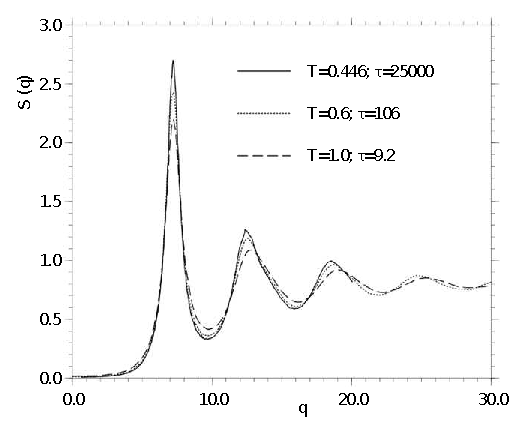
\includegraphics[width=0.8\textwidth]{sq_kob}
	\caption{The static structure factor $S(q)$ in a Lennard-Jones liquid at three different temperatures. The relaxation time $\tau_R$ increases by almost 4 orders of magnitude, and yet the structure factor shows no particular change. (from \citep{Kob2002})}
	\label{fig:rdf_glass}
\end{figure}

%\begin{figure}
%	\centering
%	\includegraphics[width=0.8\textwidth]{kawasaki_rdf}
%	\caption{$\phi$-dependence of the radial distribution function g(r) for $\Delta = 0\%$ and $\Delta = 6\%$. The blue colour means disordered, whereas the red colour means ordered. Comparison of left and right tells us that there is no disorder–order transition for $\Delta = 6\%$. However, we can see the splitting of the second peak at high $\phi$ even for $\Delta = 6\%$ (see the arrows), indicating the possible existence of medium-range order.}
%	\label{fig:rdf_glass}
%\end{figure}

\subsection{Glass or supercooled?}
\label{sec:glass_or_sc}
Following \citet{cavagna2009supercooled}, let us make here a clear semantic distinction. The glass is fundamentally out of equilibrium, whereas the supercooled liquid is in a metastable equilibrium.

The supercooled liquid is by definition metastable to the crystal. However, we can experimentally equilibrate a liquid in its metastable phase, in such a way that time-translation invariance (and thus the dynamical fluctuation dissipation theorem) holds. In such situation, no experimental measurement is able to tell us that the system is metastable. Only an explicit crystallization of the sample would unveil metastability. Therefore, with a slight abuse of language, we will call this the \emph{equilibrium} liquid phase, supercooled or not depending on whether we are below or above the melting temperature. As always in first-order phase transitions, there is no way to experimentally detect the presence of the transition temperature, as long as the system remains equilibrated into one of the two phases.

As we have seen before, the time translation invariance does not hold below $T_g$. We will use the noun "glass" and the adjective "glassy" to design the out of equilibrium solid resulting of the dynamical arrest and its phenomenology, like ageing.

%
%\begin{description}
%	\item[$T_m$] The melting point, where a first-order phase transition between liquid and crystal occurs;
%	\item[$T_c$] Goldstein's crossover temperature from a high-T nonactivated dynamics to a low-T activated one;
%	\item[$T_g$] The dynamic glass transition, where the relaxation time exceeds the conventional experimental time of \unit{10^3}{\second}, the longer the available experimental time, the lower the temperature where the system falls out of equilibrium forming a glass;
%	\item[$T_K$] Kauzmann's entropy crisis temperature, where the extrapolated liquid entropy hits the crystal entropy, and where according to some theories there is a thermodynamic phase transition;
%	\item[$T_0$] The temperature where the \ac{VFT} fit locates a divergence of the relaxation time. Often identified with $T_K$
%\end{description}

\section{Supercooled liquid dynamics}
\label{sec:sc_dynamics}

\subsection{Dynamic quantities}
\label{sec:isf_msd}

To define the dynamics of a time-dependent quantity $a(t)$, we need to measure it at two times: $t_0$ and $t_0+t$. For instance, a displacement is defined as the difference in position of the same object at two different times. 
\begin{equation}
	\Delta \vec{r}(t_0, t) = \vec{r}(t_0+t) - \vec{r}(t_0)
	\label{eq:displacement}
\end{equation}
with $\vec{r}(t0)$ the vector position of the object at time $t_0$.

In a statistical system, we often need to define an ensemble averaged dynamic correlation function:
\begin{equation}
	\mathcal{C}(a)(t_0, t) \equiv \left\langle a(t_0) \cdot a(t_0+t) \right\rangle
	\label{eq:correlation}
\end{equation}

If we deal with a statistical mechanic system at equilibrium, the ensemble average of the dynamic quantity should not depend on $t_0$, but still depend on the time lag $t$. However, one must keep in mind that $t$ is a difference between times, and not an absolute time. 

Until now, we used the relaxation time $\tau_R$ or the viscosity $\eta$ as our dynamical variable. We could have used equivalently the diffusion constant $D$. The common point of all these quantity is that they correspond to the integral of dynamical functions over all the (accessible) time lags. For instance, the relaxation time at the wavevector $q$, \latin{i.e.} at a scale $\sim \pi/q$, is the integral of the self \ac{ISF}:
\begin{equation}
	F_s(q,t) \equiv \frac{1}{N} \Bigl\langle\sum_{i=1}^N e^{-\imath\vec{q}\cdot\bigl(\vec{r_i}(t)-\vec{r_i}(0)\bigr)}\Bigr\rangle
	\label{eq:isf}
\end{equation}
where we recognise a time correlation function. The corresponding observable is $\exp{\left(\imath\vec{q} \cdot \vec{r_i}(t)\right)}$, the Fourier transform of the density fluctuations of the particle $i$. In an ergodic system, the self \ac{ISF} should decay to $0$ with a characteristic time equal to $\tau_R$, but not in a solid (crystal or glass) where it saturates at a finite value.

Another useful function, in real space this time, is the \ac{MSD}:
\begin{equation}
	\Delta r(t)^2 = \left\langle\| \vec{r_i}(t)-\vec{r_i}(0)\|^2\right\rangle
	\label{eq:msd}
\end{equation}

At very short times, the trajectory of the particles is ballistic: the particles do not influence each-other. We have $\Delta r(t)^2 \sim t^2$. In a solid the \ac{MSD} saturates to a constant value that corresponds to the amplitude of the vibration of the particles. In a liquid the particles diffuse, so at long times we have $\Delta r(t)^2 \sim D t$.

\subsection{Two step relaxation}
\label{sec:2steps}

\begin{figure}
	\centering
	\subfloat
		[Self \acs{ISF} evaluated at the value of q where the static structure factor has the main peak. At high temperatures the decay is exponential, but when the temperature get close to $T_g$ a plateau is formed and relaxation proceeds in two steps. Source \citep{Kob1995}]
		{\label{fig:isf_kob}\def\svgwidth{0.5\textwidth}\input{isf_kob.pdf_tex}}
	\subfloat
		[The \acs{MSD}. At high temperature there is a crossover from ballistic transport to diffusion. At low temperatures this crossover is interrupted by a plateau similar to what happens for the self \acs{ISF}. Source \cite{kob1995tmc}]
		{\label{fig:msd_kob}\includegraphics[width=0.5\textwidth]{msd_kob}}
	\caption{Typical dynamics of a supercooled liquid, here a binary Lennard-Jones system. Note that the time scales are logarithmic.}
	\label{fig:dynamics_kob}
\end{figure}

At high temperatures, the self \ac{ISF} decays exponentially. \FigureRef{fig:isf_kob} shows how this behaviour changes with supercooling. When decreasing the temperature a plateau appears in the correlation function that stretch to longer and longer times when approaching the glass transition. We can define two relaxation processes:
\begin{description}
	\item[The $\beta$-relaxation] appends at short times and leads to the plateau.
	\item[The $\alpha$-relaxation] is the decay from the plateau at long times.
\end{description}

The two step relaxation process is the signature of the supercooled liquid dynamics. When a plateau appears in a dynamic correlation function, a glass transition is near. We have an equilibrium measurement that informs us about the glass transition. This means that the glass transition is a physically meaningful concept.

The $\beta$-relaxation does not depend much on the temperature: the plateau is reached in comparable times at shallow and deep supercooling. However the time needed to leave the plateau gets longer by orders of magnitude and is the main cause of the divergence of the relaxation time $\tau_R$.

Obviously, the relaxation of the system cannot be described by a single relaxation time. In a first approximation, we can define a $\tau_\beta$ and a $\tau_\alpha$. The latter is the dominant relaxation time of supercooled fluids. From now on, we will use the expression "relaxation time" indifferently about $\tau_R$ at high temperature or $\tau_\alpha$ when the two step relaxation can be defined.


\subsection{Cage theory}
\label{sec:cage}

To understand more easily what the two step relaxation means in real space, we can have a look a the \ac{MSD} (see \FigureRef{fig:msd_kob}). At high temperature, we have a smooth transition between a ballistic regime where $\Delta r(t)^2 \sim t^2$ and a diffusion regime where $\Delta r(t)^2 \sim t$. The displacement corresponding to this transition is the mean free path of the particles, \latin{i.e.} the distance a particle can go without colliding with an other.

At lower temperatures, we see once again a plateau that intercalates just between the two regimes. The particle has encountered many collisions but does not diffuse. If we look at the actual value of the \ac{MSD} in correspondence of the plateau, we discover that it is quite small, well below the (square) inter-particle distance~\citep{kob1995tmc} and does not evolve much with temperature.

From theses facts emerges a quite simple picture: the particle cannot diffuse because it is always colliding into its neighbours. It is like the particle was trapped in a \emph{cage} formed by its neighbours. The plateau corresponds to the time passed in the cage. At long time the particle eventually escapes its cage and the diffusion behaviour is recovered. Don't forget that the time is in logarithmic scale: after the particle has got out of the cage, it is effectively out of any cage.

\begin{figure}
	\centering
	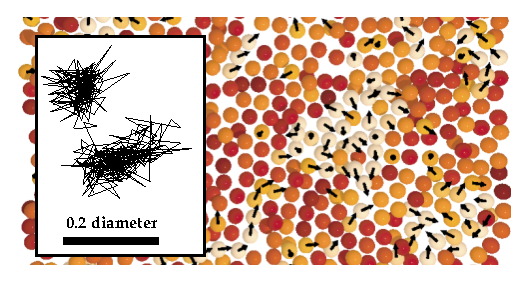
\includegraphics[width=\textwidth]{cage_weeks}
	\caption{A cut through a three-dimensional hard sphere colloidal supercooled liquid observed by confocal microscopy. The arrows indicate the direction of motion for particles with displacements superior to a tenth of diameter during a time corresponding to the middle of the plateau. The arrows are all the same length in three dimensions, so shortened arrows indicate motion in or out of the picture. Lighter colours indicate particles with larger displacements. Inset: A trajectory of one particle from this sample exhibiting cage hopping. Source \citep{weeks2002pcr}}
	\label{fig:cage_weeks}
\end{figure}

This phenomenon was observed experimentally at the microscopic level by the same sort of techniques we will be using is this thesis (see \ChapterRef{ch:Experimental} and \ChapterRef{ch:tracking}). As displayed in \FigureRef{fig:cage_weeks}, \citet{weeks2002pcr} observed indeed the particles rattling in their cages. The displacement due to a single hoping process between cages proved to be only a fraction of the inter-particle distance.

The cage theory can be mapped back to the correlation function: the $\beta$-relaxation is interpreted as the motion between two collision with the neighbours; the plateau indicates that the particle position does not decorrelate further during all the time spent in the cage; the $\alpha$-relaxation corresponds to the escape from the cage and the recovery of ergodicity.

However useful is the picture of the cage to describe what happens in supercooled liquid, it is neither explicative nor complete. We don't know why the neighbours begin to form cages when supercooling the system, and why the frequency of cage hopping decreases at least exponentially with temperature when approaching $T_g$. Furthermore, the right picture is maybe not a particle breaking its cage but a group of particles rearranging cooperatively~\citep{Kob1997, Donati1998, Donati1999, kegel2000swe, Perera1999, weeks2000, weeks2002pcr} as suggested by the clusters and strings of moving particles displayed in \FigureRef{fig:cage_weeks}.

\subsection{Non-Gaussian distribution of the dynamics}
\label{sec:nongaussian}

The major drawback of the cage picture is that it considers all particles as equivalent, diffusing independently at the same rate. If this picture was true, the distribution of the displacements should be Gaussian. This proves to be wrong, as displayed in \FigureRef{fig:not_gaussian}.

\begin{figure}
	\centering
	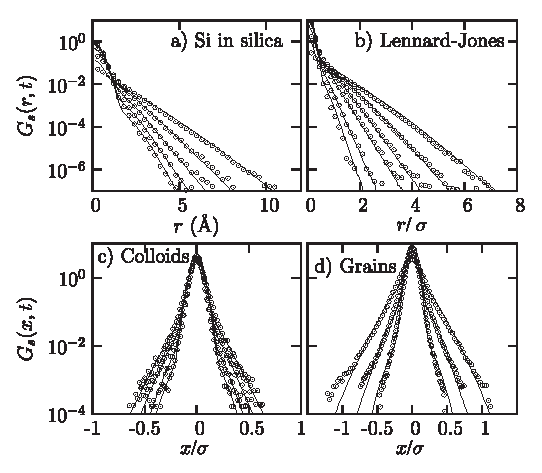
\includegraphics[width=0.8\textwidth]{not_gaussian}
	\caption{Time evolution of the distribution of the displacements for silicon atoms in silica, Lennard-Jones particles, hard-sphere colloids, and grains (open circles), fitted with a combination of a Gaussian for the central part and broad exponential tails (full lines). From~\citep{Chaudhuri2007}}
	\label{fig:not_gaussian}
\end{figure}

The distribution of the displacements is not Gaussian, it has fat exponential tails for large displacement. This is interpreted as the existence of two distinct populations of particles: localized particles that contribute to the central Gaussian distribution and mobile particles that contribute to the exponential tails. A particle that was able to jump out of its cage recently is much more likely to jump again than a particle that has been localised for some time. Jumping evens are not independent.

To quantify such a non-gaussianity of a distribution, the relevant quantity is its (reduced, normalized) fourth moment, the kurtosis often called the \ac{NGP}. In the case of the displacement, it is expressed from the mean square and mean quadratic displacements
\begin{equation}
	\alpha_2(t) \equiv \frac{3 \left\langle {\Delta r}^4(t) \right\rangle}{5 {\left\langle {\Delta r}^2(t) \right\rangle}^2}-1
	\label{eq:ngp}
\end{equation}
Once again, $t$ is a time difference from an arbitrary reference time $t_0$. This function has a more and more pronounced bell shape when approaching the glass transition (see \FigureRef{fig:ngp_kob}). The \ac{NGP} starts to increase on the time scale of the $\beta$-relaxation, reaches its maximum and starts to decrease on the time scale of the $\alpha$-relaxation. The maximum of the \ac{NGP} corresponds to the end of the plateau and appends at later and later times with decreasing temperature.

The decrease to zero of the \ac{NGP} at long times is physically meaningful: the distinction between mobile and localised particles is only transient. If we integrate the displacements over long enough time, all the particles are alternatively localised and mobile.

\begin{figure}
	\centering
	\subfloat
		[\acl{NGP} function of time with increasing supercooling. From~\citep{Kob1997}.]
		{\label{fig:ngp_kob}\includegraphics[width=0.5\textwidth]{ngp_kob}}
	\subfloat
		[Time and temperature dependence of the dynamical correlation length $\xi_4(t)$. From~\citep{Lacevic2003}.]
		{\label{fig:xi4}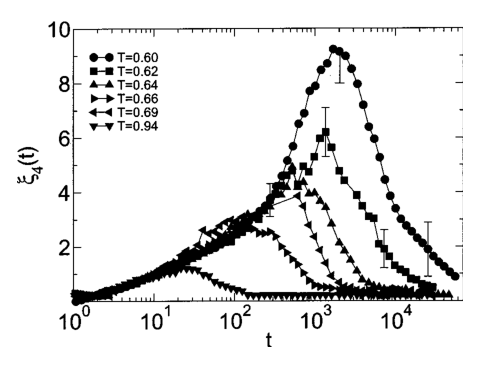
\includegraphics[width=0.5\textwidth]{xi4_lacevic}}
	\caption{Non-gaussianity of the dynamics and corresponding dynamical correlation length in a binary Lennard-Jones system.}
\end{figure}


The non-gaussianity of the displacements translates into a distribution of time scales for the $\alpha$ relaxation. Indeed, the long time part of the self \ac{ISF} is not a single exponential. It is rather well fitted by the Kohlraush-Williams-Watts~\citep{Kohlrausch1847, Williams1970} stretched exponential form $A \exp{\left[ -\left( t/\tau_\alpha \right)^\beta\right] }$ with $\beta<1$ the stretching exponent and $A$ the height of the plateau, also called the Debye-Waller factor. As a whole, the self \ac{ISF} can be fitted as:
\begin{equation}
	F_s(q,t) \sim (1-A) \exp{\left[-\frac{t}{\tau_\beta}\right] } + A \exp{\left[ -\left( \frac{t}{\tau_\alpha} \right)^\beta\right] }
	\label{eq:streched_exp_2steps}
\end{equation}

With this definition, the \ac{NGP} reaches its maximum at a time scale a few times smaller than $\tau_\alpha$. Then, the value of the self \ac{ISF} approximatively corresponds to the Debye-Waller factor.

\subsection{Dynamic Heterogeneities}
\label{sec:dynhet}

\begin{figure}
	\centering
	\subfloat
		[Dynamic heterogeneities in a 2D supercooled liquid simulation. Plot of the end-to-end particle displacement vectors. From~\citep{Perera1999}]
		{\label{fig:dh_perera}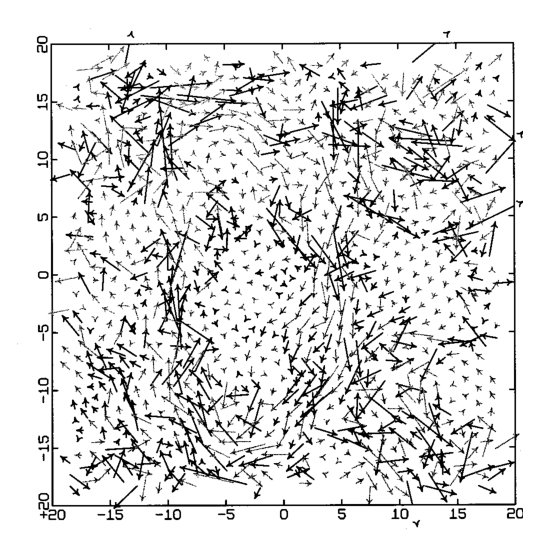
\includegraphics[width=0.5\textwidth]{dh_perera}}
	\subfloat
		[Dynamic heterogeneities in hard sphere supercooled liquid experiments. The locations of the fastest particles (large spheres) and the other particles (smaller spheres).  From~\citep{weeks2000}]
		{\label{fig:dh_weeks}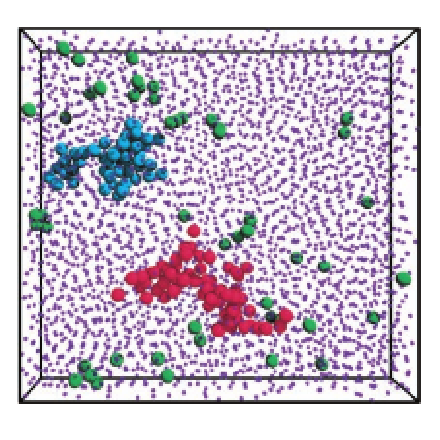
\includegraphics[width=0.5\textwidth]{dh_weeks}}
	\caption{Visualisation of dynamic heterogeneities. When calculated according to the appropriate time scale $t^{dh}$, the displacements of the particles show heterogeneities in space. In \subref{fig:dh_weeks} the particles all have the same physical size, which is the size of the large spheres.}
	\label{fig:dynhet}
\end{figure}

As we said at the end of \SectionRef{sec:cage}, the relaxation in a supercooled liquid is not a single-particle process; it involves a group of particles that have to rearrange cooperatively. This notion articulates with the non-gaussianity of the dynamic to give the notion of dynamic heterogeneities: groups of particles rearrange cooperatively many times which yields a high mobility for these particles, when other regions of the system are not rearranging implying that the particles there are localised~\citep{Kob1997, Donati1998, Donati1999, kegel2000swe, Perera1999, weeks2000, weeks2002pcr}.

The dynamic heterogeneities are best observed (see \FigureRef{fig:dynhet}) when calculating the value of dynamical functions at the maximum of the \ac{NGP}. We note the time scale of this maximum $t^{dh}$. Once again, we need two times (or a difference of times) to describe the physics of the system. Even more interesting is the size of the dynamic heterogeneities that is increasing when approaching the glass transition (see \FigureRef{fig:xi4}).


\subsection{How to define a dynamical length scale}
\label{sec:dyn_length}
To define the characteristic length scale of the dynamic heterogeneities, \citet{Donati1999} thought about correlating in space the displacements $\Delta r_i(t) = \vec{r}_i(t)-\vec{r}_i(0)$ or more precisely, the fluctuations of the norm of the displacements $\delta u_i(t) = \Delta r_i(t) - \left\langle \Delta r_i(t) \right\rangle$. The mobility-mobility spatial correlation function is defined as:
\begin{equation}
	\mathcal{G}_{u(t)}(r) \equiv \mathcal{G}_u(r,t) \equiv \frac{
		\left\langle \sum_{i,j}{\delta u_i(t) \delta u_j(t) \delta(r_{ij} -r)} \right\rangle 
	}{
		\left\langle \sum_{i,j}{\delta(r_{ij} -r)} \right\rangle
	}
	\label{eq:mobility_correl}
\end{equation}

Note that for $r=0$ \EquationRef{eq:mobility_correl} boils down to the \ac{MSD} (\EquationRef{eq:msd}). $\mathcal{G}_u(t,r)$ informs us about the spatial fluctuations of the \ac{MSD}. The four-point correlation function that corresponds in the same way to the spatial fluctuations of the \ac{ISF}~\citep{Lacevic2003} is 
\begin{equation}
	 \mathcal{G}_4(r, t) \equiv 
	 	\left\langle \delta\rho(0,0)\delta\rho(0,t) \delta\rho(r,0)\delta\rho(r,t) \right\rangle 
	 	- \left\langle \delta\rho(0,0)\delta\rho(0,t) \right\rangle 
	 		\left\langle \delta\rho(r,0)\delta\rho(r,t) \right\rangle
	 \label{eq:four_point_correl}
\end{equation}

The name "four-point correlation function" stands for the $4$ points needed to defined such a function: $r_i(t_0)$, $r_i(t_0+t)$, $r_j(t_0)$ and $r_j(t_0+t)$. We can define a susceptibility for each of these functions,
\begin{align}
	\chi_u =& \int{dr \mathcal{G}_u(t,r)} \label{eq:dynamic_susc}\\
	\chi_4 =& \int{dr \mathcal{G}_4(t,r)} \label{eq:chi4}
\end{align}
and a correlation length $\xi_u(t)$, $\xi_4(t)$ from the decay of the correlation function. The largest susceptibility and the longer correlation length can be obtained for $t=t^{dh}$ (see \FigureRef{fig:xi4}). Thus from now on if $t$ is omitted in a four-point observable, it means $t=t^{dh}$.


\section{A static cause to dynamic heterogeneities?}
\label{sec:static_cause}

\subsection{The quest for a static length scale}
\label{sec:static_length}

We saw in \SectionRef{sec:X+glass} that the usual static correlation function where not changing significantly when approaching the glass transition. Nothing spectacular happens in the positional order of the system when simultaneously its dynamics slows down by many orders of magnitude. In critical phenomena a static correlation length (the characteristic size of the critical fluctuations) diverges, which are responsible for the dramatic slowing down of the system: the larger, the slower. No diverging static correlation length could be found for decades in glass forming liquids.

In \SectionRef{sec:dynhet} and \SectionRef{sec:dyn_length} we saw that a dynamic correlation length can be defined corresponding to dynamic heterogeneities in the system. If we could find a static cause to the dynamic heterogeneities, its length scale is likely to increase in the same way as the dynamic correlation length, achieving the quest for a static length diverging at the glass transition.

In this section, we will review the body of evidence that points toward the existence of a static cause, whatever it is, to the dynamic heterogeneities.

\subsection{Dynamic propensity}
\label{sec:propensity}

\begin{figure}
	\centering
	\includegraphics[width=0.8\textwidth]{propensity}
	\caption{Dynamic propensity map of a 2D soft disk simulation. From~\citep{Widmer-Cooper2005}}
	\label{fig:propensity}
\end{figure}

It is quite natural to think that a rearrangement at a given place will trigger other rearrangements nearby because it offers new possibilities of motion. It is thus difficult to disentangle the influence of the static structure from the the consequences of previous dynamical events. To address this point, \citet{Widmer-Cooper2005} introduced the iso-configurational ensemble and the dynamic propensity.

The iso-configurational ensemble is a simulation trick to get rid of the influence of the initial dynamics. \citet{Widmer-Cooper2005} ran $M$ simulations with the same starting configuration but with momenta assigned randomly from the appropriate Maxwell–Boltzmann distribution. If $M$ is large enough, the average over those runs of any observable should be depending only on the initial configuration. If the iso-configurational averaged observable is spatially homogeneous, then this observable do not depend on the initial configuration.

\citet{Widmer-Cooper2005} named \emph{dynamic propensity} the iso-configurational average of the square displacement, because it does not correspond to the actual squared displacement of the particle in any particular run but, rather, reflects the particle's propensity for displacement. As shown in \FigureRef{fig:propensity}, the propensity is heterogeneous, so the structure can predict the propensity. Subsequent works focused mainly on the predictability of the propensity by the structure~\citep{Widmer-Cooper2007, Matharoo2006, Coslovich2006, Appignanesi2006, RodriguezFris2007, Hedges2007, Downton2007}.

\subsection{Predicting the dynamics}

\citet{Berthier2007} showed that the propensity was in fact a poor predictor of the dynamics at the particle level. In particular, the distinction between fast and slow particles is no longer apparent after iso-configurational average. So the link between structure and dynamics \latin{via} the propensity seems to be broken. 

However the same authors show that at larger scales the dynamic propensity predicts well the size and the geometry of the dynamic heterogeneities. While it is not possible to use the structure to predict whether a given particle will be fast or slow in a single run, it is possible to tell if it belongs to a fast or slow region.

In particular, the structure should be able to predict the diverging size of the dynamic heterogeneities. So the quest for a static diverging length scale is not vain.

\subsection{What sort of static cause?}

Even if we know that the initial positions of the particles plays a role in the dynamic heterogeneities, the precise static features that control the dynamics are still to be determined. Various attempts have been made in this direction, considering the elastic properties~\citep{Brito2006, Widmer-Cooper2008, Tsamados2009}, the configurational entropy~\citep{adam1965tdr, Kirkpatrick1987a, Kirkpatrick1987, kirkpatrick1989scd}, or through the idea of a rough energy landscape~\citep{Stillinger1984}. These approaches often focus on the rearranging regions, trying to understand why, when and how they rearrange.

Another line of thought is to focus on the slow regions and understand why they are not rearranging. After all, the specificity of the glass transition is a slowing down, not that particles move. The notion that some stable structures form in the supercooled liquid emerges quite naturally. However, the term "structure" has to be defined properly. We said in \SectionRef{sec:X+glass} that the usual definition of order, well adapted to distinguish between a long-range positionally ordered crystal and the disordered high temperature liquid, was not sufficient to detect the onset of the glass transition. The structure that may exist in supercooled liquid must then be local or medium-ranged and not detectable by the usual two-point density correlation methods.

The frustration-based approach~\citep{tarjus2005fba} postulates the existence of a local order in any liquid, order that cannot tile the whole space, for instance the $5$-fold symmetry. Without this geometric frustration, the order would fill space and be at even lower energy than the crystal. The partial ordering despite frustration would be the origin of the slowing down.

\begin{figure}
	\centering
	\subfloat[$\psi_6$]{\label{fig:kawa_nm_psi6}\def\svgwidth{0.3\textwidth}\input{kawa_nm_psi6.pdf_tex}}
	\subfloat[$\Delta r^2$]{\label{fig:kawa_nm_msd}\def\svgwidth{0.3\textwidth}\input{kawa_nm_msd.pdf_tex}}
	\subfloat[$Q_6$]{\label{fig:kawa_nm_3d}\def\svgwidth{0.3\textwidth}\input{kawa_nm_3d.pdf_tex}}
	\caption{\subref{fig:kawa_nm_psi6} fluctuations of the crystal-like bond order parameter in polydisperse quasi hard disks simulations and \subref{fig:kawa_nm_msd} the corresponding dynamic heterogeneities. \subref{fig:kawa_nm_3d} Same as \subref{fig:kawa_nm_psi6} in 3D, but the low order particles are not shown for clarity. From~\citep{tanaka2010critical}.}.
	\label{fig:kawa_nm}
\end{figure}

Tanaka~\cite{tanaka1999top,Tanaka1999} noticed that the avoided crystallisation should not be forgotten in the supercooled branch. By definition a supercooled liquid is metastable to a crystal and the underlying tendency to crystalline ordering must be important. The avoidance of crystallisation, the dynamical arrest and the fragility can be all linked by using two order parameters that account respectively for the tendency toward global ordering (crystallisation) and the formation of locally favoured structures incompatible with the crystal symmetry. The term "frustration" is also used in the two order parameter model, but it is related to the frustation on the way to crystallisation~\citep{tanaka2005top, Tanaka20053371, Tanaka20053385, Shintani2006}, not to a type of order intrinsically frustration by the geometry of space.

Tanaka and co-workers~\citep{kawasaki2007cbd, Shintani2006, watanabe2008, Kawasaki2010} showed that in various systems (simulations and 2D granular matter experiments) the fluctuations of the local crystalline order are closely related to dynamic heterogeneities (see \FigureRef{fig:kawa_nm}). Moreover, the length scale of these fluctuations show an Ising-like power-law divergence toward the glass transition point~\citep{tanaka2010critical}. These results suggest a far more direct link than thought before between the glass transition and critical phenomena. Indeed, the glass transition may be a new type of critical phenomenon where a structural order parameter is directly linked to slowness. Furthermore, this structural ordering accompanies little change in density, which explains why it has not been detected by the static structure factor so far.

The present work is based on these results and try to test and extend them in 3D by experiments.


\section{Hard spheres and colloids}
\label{sec:HS-colloids}

The experimental systems that allow to to probe directly their local structure are few. The present section introduces one of them that is investigated in this thesis: colloidal hard spheres.

\subsection{Crystallisation and glass transition}

\begin{figure}
	\centering
	\def\svgwidth{0.9\textwidth}
   	\input{phase_diagram.pdf_tex}
	
	\caption{Behaviour of almost identical hard spheres upon increasing volume fraction from 0.4 (usual liquid) to 0.74 (close packing). Top: Equilibrium phase diagram for the monodisperse system. Bottom: metastable branch with respect to the avoided crystallisation for $6\%$ polydispersity.}
	\label{fig:HS_phase_diagram}
\end{figure}

Hard spheres are defined as impenetrable spheres. Apart from this no overlap condition, they have neither repulsion nor attraction between them, so no potential energy. This very simple definition makes this theoretical object a cornerstone of statistical mechanics, and it has been subjected to an exceptional degree of interest, to the extent that hard spheres form one of the best understood systems of condensed matter. In particular, a first order fluid-to-crystal freezing transition of hard spheres was discovered more than 50 years ago in the early computer experiments of \citet{wood1957} and \citet{alder1957}.

Hard sphere crystallization is puzzling. Why would a system without potential energy, driven only by entropy, prefer order to disorder? The answer was suggested by \citet{hoover1958}: a globally ordered configuration allows more vibration of each particle than a disordered configuration. In terms of \EquationRef{eq:config_vib}, the crystallisation decrease the configurational entropy $S_c$ but increases the vibrational entropy $S_{vib}$. At high enough density $|\Delta S_c|<|\Delta S_{vib}|$ so the entropy paradoxically increases upon (global) ordering.

Not long after this discovery, drawing on their own free-volume theories and sphere packing experiments~\citep{Scott1960, Bernal1960}, \citet{Cohen1959, Cohen1964} suggested that compressing an assembly of hard spheres fast enough to by-pass crystallization should result in a metastable, amorphous, solid "glass" state. In 1986, experiments by \citet{pusey1986} on suspensions of colloidal particles that interact via a steep repulsive potential observed both the freezing transition and, at higher concentrations, glass formation.

\subsection{Equations of state}
\label{sec:eos}

In the case of the single component hard sphere fluid, the osmotic pressure is well-approximated by the Carnahan-Starling \ac{EOS}~\citep{carnahan1969},
\begin{equation}
\frac{PV}{N k_B T}=\frac{1 + \phi + \phi^2 - \phi^3}{(1 - \phi)^3}
\label{eq:CS}
\end{equation}
where $P$ is pressure, $V$ is volume, $N$ is the number of particles within $V$ and $\phi$ is the volume fraction defined as 
\begin{equation}
	\phi \equiv N \frac{\pi\sigma^3}{6 V}
	\label{eq:vf_mono}
\end{equation}
where $\sigma$ is the hard core diameter. The volume fraction is the only control parameter of the phase behaviour of monodisperse hard spheres. When comparing between hard spheres and systems having a potential energy, one may think about the volume fraction as an inverse temperature: increasing the volume fraction is somewhat equivalent as cooling a thermal system. At $\phi=\phi_m \equiv 0.4954$ monodisperse hard spheres freeze and at $\phi=\phi_X \equiv 0.5478$ they melt. At higher volume fractions one finds a kinetic glass transition volume fraction $\phi_g$ before reaching an theoretical ideal glass transition at $\phi_0$. In general, all the relations that we presented in the previous sections of this chapter can be adapter to the case of hard spheres by changing $T$ in $1/\phi$.

The osmotic pressure of the single component hard sphere crystal is well approximated by the form given by \citet{hall1972}.
\begin{equation}
\frac{PV}{N k_B T} = \frac{
1 + \phi + \phi^2 - 0.67825 \phi^3 - \phi^4 - 0.5 \phi^5 - 6.028 e^{\phi\epsilon(7.9-3.9\phi\epsilon)}\phi^6
}{
1 - 3 \phi + 3 \phi^2 - 1.04305 \phi^3
}
\label{eq:Hall}
\end{equation}
where $\epsilon=\phi_{cp}/\phi -1$ quantifies the distance to the close packing volume fraction $\phi_{cp} = \pi\sqrt{2}/6 \simeq 0.74$. The parametrization given by \citet{Young1979} is also often used for its simplicity even though it deviates from Hall's for small $\phi$.
\begin{equation}
\frac{PV}{Nk_{B}T} = \frac{3}{\epsilon} + 2.566 + 0.55 \epsilon - 1.19 \epsilon^2 + 5.95 \epsilon^3
\label{eq:Alder}
\end{equation}

\subsection{Colloidal hard spheres}
\label{sec:colloidalHS}
In addition to their fundamental simplicity, hard spheres have been very closely approximated experimentally using colloidal dispersions. \ac{DLVO} theory suggests that the stability of a colloidal dispersion depends on the sum of the attraction and repulsion potential (\FigureRef{fig:DLVO-a}). the attractive component is usually due to short ranged van der Waals forces. It causes irreversible aggregation of the colloids. The repulsive interaction potential is long ranged and due to the electrostatic double layer made of the charge on the colloids and of the counter ions in the solvent. The range of this repulsive potential is the Debye length. Adding salts to the solvent is diminishing the Debye length. In aqueous media, it will easily destabilize the colloidal dispersions, making it fall into the primary minimum due to the van der Waals interaction. In non-aqueous media, the dielectric constant is weaker so the Debye length is never short enough to have an unstable colloidal dispersion. On the contrary, the double layer energy can be enforced by adding salts to the solvent, stabilizing the suspension.

\begin{figure}
	\centering
	\subfloat[Free energy variation function
of the particle separation.]{\label{fig:DLVO-a}\def\svgwidth{0.4\textwidth}\input{dlvo_theory_1.pdf_tex}}
	\subfloat[In the case of highly charged solutions,
a second minimum appears.]{\def\svgwidth{0.4\textwidth}\input{dlvo_theory_2.pdf_tex}}
	\caption{\acl{DLVO} theory.}
	\label{fig:DLVO-theory}
\end{figure}

The key to approximate hard spheres with almost uncharged colloidal dispersions is the steric stabilization~\citep{pusey1986}. Polymers are adsorbed or even bind to the colloids to keep their surface further apart than the van der Waals attraction range, preventing aggregation.

\subsection{Polydispersity}
\label{sec:poly}
The usual way to avoid crystallisation of spherical particles is to mix two or more types of particles, like in the well known Kob-Anderson binary mixture of Lennard-Jones particles~\citep{kob1995tmc}. Colloids naturally present a distribution of sizes, often approximated as Gaussian. Monodisperse colloids are impossible but can be approximated as close as $3\%$ polydispersity. 

This experimental constrains motivated investigations about the effect of polydispersity on the phase behaviour of hard spheres by experiments~\citep{pusey1986, pusey}, computer simulations~\citep{Dickinson1985, Bolhuis1996, Phan1998}, density functional theories~\citep{Barrat1986, McRae1988}, and simplified analytical theories~\citep{Barrat1986, Pusey1987, McRae1988, Bartlett1997, Sear1998, bartlett1999, Xu2003}. These studies have revealed that, compared to the monodisperse case, polydispersity causes several qualitatively new phenomena. 

It is intuitively clear~\citep{Pusey1987} that significant diameter polydispersity should destabilize the crystal phase, because it is difficult to accommodate a range of diameters in a lattice structure. Polydispersity induces geometrical frustration against crystallisation. Experiments indeed show that crystallization is suppressed above a terminal polydispersity of $\Delta_t \simeq 12\%$~\citep{pusey1986, pusey}. Theoretical work suggested that this arises from a progressive narrowing of the fluid-solid coexistence region with increasing $\Delta$, with the phase boundaries meeting at $\Delta_t$~\citep{McRae1988, Bartlett1997} in a point of equal concentration~\citep{bartlett1999}. \citet{Fasolo2003} refined the previous determinations of $\Delta_t$ by taking into account the fractionation into several solid phases that occurs at sufficiently large polydispersity. They found $\Delta_t \simeq 7\%$.

Kawasaki \latin{et al.} showed in simulation that polydispersity also affects the fragility of (almost) hard disks~\citep{kawasaki2007cbd} and (almost) hard spheres~\citep{Kawasaki2010}. Higher polydispersity induces stronger glass. Frustration against crystallization has been shown to decrease fragility in various other systems~\citep{tarjus2005fba, Shintani2006, molinero2006tts, Coslovich2007, watanabe2008, tanaka2010critical}. So the polydispersity~$\Delta$, which controls the degree of frustration against crystallization, governs not only glass-forming ability, but also the fragility, or the glass transition behaviour.

\subsection{Simulation data}
\label{sec:sim_kawa}

In this thesis we will sometimes re-analyse the simulations ran by Takeshi Kawasaki~\citep{tanaka2010critical, Kawasaki2010}.

From his data, we used the closest from our experiments that were available: \ac{BD} simulations of hard-sphere-like particles interacting with the \ac{WCA} repulsive potential
\begin{equation}
	U_{jk}(r) = \left\{\begin{array}{l l}
  		4\epsilon\left[ \left( \frac{\sigma_{jk}}{r}\right)^{12} - \left( \frac{\sigma_{jk}}{r}\right)^{6} +\frac{1}{4}\right]  & \quad \text{for $r<2^\frac{1}{6} \sigma_{jk}$}\\
  		0 & \quad \text{otherwise}
  	\end{array} \right.
	\label{eq:WCA}
\end{equation}
where $\epsilon$ gives the energy scale, $\sigma_{jk} = (\sigma_j + \sigma_k)/2$. The effective diameter of the particle is defined where the potential energy becomes equal to the thermal energy:
\begin{equation}
	U(\sigma_{eff}) = k_B T
\end{equation}
where $k_B$ is the Boltzmann constant. The temperature is fixed at $k_B T/\epsilon = 0.025$. The volume fraction is calculated using $\sigma_{eff} = 1.095\sigma$.

Unless mentioned otherwise, the size polydispersity is Gaussian with $\Delta=6\%$.

\section{Aim and plan}

Our goal in this thesis is to investigate the structures appearing in a hard sphere liquid upon supercooling and to make the link between some of these structures and the dynamic heterogeneities. Thus, we may be able to describe the glass transition by the mean of a static (structural) characteristic size that would diverge at an ideal glass transition volume fraction.

The body of this thesis is divided into two parts. In the first one we explain the methods, original or from the literature, that are used in the second part to output results about the structure of our system (\ChapterRef{ch:structure}), its dynamics and the relationship between the two (\ChapterRef{ch:results_dynamics}). The closely related matter of crystallisation will be discussed in \ChapterRef{ch:crystallisation}.
	\svnidlong
{$HeadURL$}
{$LastChangedDate$}
{$LastChangedRevision$}
{$LastChangedBy$}
\svnid{$Id: $}

\chapter{Experimental}
\label{ch:Experimental}


\section{Colloid synthesis}
\label{sec:synthesis}

Our method to synthesize fluorescently labeled and sterically stabilized \ac{PMMA} colloids is mainly based on the Pine sythesis~\citep{klein2003} but is also inspired of works by \citet{antl1986} and \citet{bosma2002}.


\subsection{Principle}

The principle of this colloid synthesis is a well controlled polymerization of Methyl-Methacrylate. The monomer dissolves easily into an apolar solvent such as Hexane. But at a certain degree of polymerization, the polymer chain becomes immiscible and collapses on itself, forming a nucleus for the colloid growth. Until the monomer is completely consumed in the reactor, the nuclei continue to grow. The growth rate is determined by the concentration of monomer and is therefore uniform for a well-stirred reactor. So, all colloid nucleus should appear at the same time, grow at the same rate and stop their growth at the same moment. This allows a production of fairly monodisperse colloids.

But the nuclei being immiscible in the solvent, they would tend to aggregate, forming a block of \ac{PMMA} instead of well dispersed spheres. Which is why the colloids must be stabilized. The stabilizer is a large molecule with a functional group looking like the monomer in order to get involved in the polymerization. That way the stabilizer is chemically bonded to the colloid and pointing outward, sterically repelling the other colloids. Therefore colloids are no longer able to aggregate, as explained in \SectionRef{sec:HS-colloids}. We used methacryloxypropyl terminated \ac{PDMS} (Mw = \unit{25000}{\gram\per\mole}) as stabilizer.

In order to get fluorescently labeled colloids, some synthesis methods only add the fluorescent dye into the reaction mixture. The dye is then trapped physically into the growing colloids, and once washed, the colloids are fluorescently labeled. The problem with this method is that the labeling is unstable. After some time in a solvent, the dye diffuses out of the colloids, leading to a more and more fluorescent solvent, to less and less fluorescent colloids and so to worse and worse quality of imaging of the sample. To avoid that, we functionalized our dyes (rhodamine B isothiocyanate or coumarine) with a methacrylate group able to polymerize into \ac{PMMA} chains. That way, we get a dye chemically bonded to the colloids and a very stable labeling.


\subsection{Experimental procedure}


\subsubsection{Preparation of the ingredients}

In order to have a well controlled initiation of the polymerization reaction, a very pure initiator is needed. We used commercial \ac{ADIB} but we recrystallized it in acetone.

Commercial monomer \ac{MMA} is sold inhibited, in order to prevent any polymerization before use. The inhibitor must be removed before use, using an inhibitor remover column. The inhibited monomer is poured thought the column and comes out free of inhibitor.

The making of dyed monomer is also a part of the preparation. We mix \ac{EGDM} with the dye (rhodamine B isothiocyanate or coumarine) in acetone and stir it during two days in a UV-screened flask. The acetone is then evaporated to get back the dyed monomer as a powder.


\subsubsection{Experimental setup of the synthesis}

The synthesis was performed in a \unit{250}{\milli\litre} three-neck flask placed in a heated silicon oil bath and stirred magnetically. The flask was equipped with two removable caps to add chemicals and a water cooled reflux condenser topped by a nitrogen inlet tube to prevent oxygen diffusing into the system.

A typical synthesis proceeds as follow: Initially \unit{0.2}{\gram} of initiator was dissolved into \unit{44}{\gram} of hexane and \unit{22}{\gram} of dodecane (less volatile). Then \unit{0.2}{\gram} of stabilizer at \unit{25000}{\gram\per\mole} was added as well as a part of the monomer (in order to have around \unit{5}{\gram} of monomer remaining). Then the flask was set under the reflux and stirred. Meanwhile, the dye was dissolved into a mixture of \unit{0.8}{\gram} of acetone (to get higher polarity and higher solubility), \unit{0.41}{\gram} of \ac{MA} and the rest of the monomer. If the dye was overdosed, the non-dissolved bits where filtered off before the dyed mixture was poured into the reactor.

Finally, polymerization stopper (\unit{1}{\milli\litre} of octanethiol) was added into the reactor. After one minute of moderate nitrogen flux, all caps were sealed and the nitrogen flux stopped. The reaction mixture is then heated to \unit{80}{\celsius} for an hour. Before reaching this temperature, flocculation of densely dyed material may occur. In this case, the heating is stopped, the reaction mixture filtered and all is put back in the same configuration and heated again to \unit{80}{\celsius}. This filtering process was annoying but seemingly had no influence on the result of the synthesis.

After 1 hour at \unit{80}{\celsius} we let the reaction mixture cool down, sedimented into an Erlenmeyer flask and then washed two times with petroleum ether to keep only the colloids.


\subsection{Testing the synthesized colloids}


\subsubsection{Qualitatively by confocal microscope}

Just after reaction, a drop of the reaction mixture is dried on a microscope slide, immersed in a drop of index matched emulsion oil and then put under the confocal microscope. Dried colloids tend to form crystals. Measuring the lattice size of those crystals gives us a qualitative idea of the size of our particles.


\subsubsection{Quantitatively by light scattering}

Static light scattering spectrum of a drop of the reaction mixture diluted in hexane is fitted to Mie theory~\citep{Bohren1983, Dhont1996}. This gives us the mean size and the polydispersity of our colloids.


\subsection{Results of the synthesis}

The different parameters we used for the synthesis and the corresponding results are given in \TableRef{tab:Result-of-synthesis}. Only the two last syntheses and the two syntheses using coumarine dye did not need filtering. We were able to obtain diameters between \unit{0.98}{\micro\meter} and \unit{1.58}{\micro\meter} with polydispersity between $4\%$ and $6.5\%$. We tried to broaden the diameter range in the last synthesis by quenching the reaction after \unit{11}{\minute} at \unit{80}{\celsius}. We could then obtain a diameter of \unit{0.38}{\micro\meter} but with a $12\%$ polydispersity.


\begin{sidewaystable}
	\centering
	
	\begin{tabular}{|r|c|c|c|c|c|c|c|c|c|c|}
	\hline RAS & \milli\gram & $\sim$25 & $\sim$25 & $\sim$25 &  &  & 13 & 5.2 & 5.8 & 5.9 \\ 
	\hline CAS & \milli\gram &  &  &  & $\sim$25 & 10.7 &  &  &  &  \\ 
	\hline \ac{ADIB} & \gram & 0.2 & 0.2 & 0.2 & 0.2 & 0.205 & 0.204 & 0.102 & 0.2054 & 0.103 \\ 
	\hline Hexane & \gram & 44 & 44 & 44 & 44 & 44.04 & 44.02 & 44 & 44.01 & 44.02 \\ 
	\hline Dodecane & \gram & 22 & 22 & 22 & 22 & 22 & 22.08 & 22.01 & 22 & 22.25 \\ 
	\hline \ac{MMA} & \gram & 20.3 & 20.3 & 20.3 & 20.3 & 20.31 & 20.29 & 10.1 & 10.04 & 10.08 \\ 
	\hline \ac{MA} & \gram & 0.4 & 0.4 & 0.4 & 0.4 & 0.41 & 0.41 & 0.22 & 0.1985 & 0.2 \\ 
	\hline acetone & \gram & 0.8 & 0.8 & 0.87 & 0.8 & 0.8 & 0.8 & 0.44 & 0.8 & 0.42 \\ 
	\hline stabilizer & \gram & 1 & 0.58 & 0.38 & 1.18 & 0.69 & 1.7 & 0.52 & 1.71 & 0.99 \\ 
	\hline octanthiol & \milli\litre & 0.1 & 0.1 & 0.1 & 0.1 & 0.1 & 0.1 & 0.05 & 0.1 & 0.1 \\ 
	\hline $\sigma$ & \micro\metre & 1.22 & 1.46 & 1.58 & 1.10 & 1.52 & 1.03 & 1.15 & 0.98 & 0.38 \\ 
	\hline $\Delta$ & $\%$ & 6 & 5 & 5 & 6 & 6.5 & 6.5 & 4 & 4 & 12 \\ 
	\hline 
	\end{tabular} 
	
	\caption{Result of colloid synthesis. The last one was quenched after 11 min. RAS stands for methacrylated rhodamine, CAS for methacrylated coumarine.}
	\label{tab:Result-of-synthesis}
\end{sidewaystable}

\section{Experimental setup}


\subsection{Samples}
\label{sec:samples}

\subsubsection{Hard Spheres colloids}
\label{subsec:colloids}
We used \ac{PMMA} colloids synthesised following the protocol detailed in \SectionRef{sec:synthesis}. The colloids are sterically stabilized with methacryloxypropyl terminated PDMS and fluorescently labelled with rhodamine isothiocyanate chemically bonded to the \ac{PMMA}~\citep{bosma2002}.

The colloids are suspended in a solvent mixture of \ac{CIS} and \ac{CHB}. Both solvents have a refractive index close to the one of \ac{PMMA} ($n_{PMMA}=1.4947$, $n_{CIS}=1.481$, $n_{CHB}=1.5052$). Refractive index matching enables us to see through a few millimetres of concentrated suspensions without suffering from multiple scattering of light and leads to very precise imaging hundreds of microns deep into our samples. Due to the steric stabilization and refractive index matching, the van der Waals interactions are reduced to a fraction of the thermal energy and can therefore be neglected. 

To screen any (weak) electrostatic interactions, we dissolved \ac{TBAB} salt, to a concentration of \unit{300}{\nano\mole\per\liter}~\citep{royall2005}. The estimated Debye screening length is \unit{100}{\nano\metre}, well below the length scale of the colloids. 

To the extent of our knowledge, the interactions between the colloids we used are as close as possible to the theoretical hard core potential for micron-sized particles.


\subsection{Size and polydispersity}
\label{sec:size_poly}
\subsubsection{On the importance of size}

Particle size determination is crucial for experiments. We saw in \SectionRef{sec:colloidalHS} that the phase behaviour and the glass transition of hard spheres is controlled by the volume fraction $\phi$ that is the volume of space occupied by the particles.
\begin{equation}
	\phi \equiv \sum_i \frac{\pi}{6}\frac{\sigma_i^3}{V} = \frac{\pi}{6}\langle \sigma^3 \rangle \rho
	\label{eq:volume-fraction}
\end{equation}
with $V$ the total volume, $\sigma_i$ the diameter of the particle $i$, and $\rho=N/V$ the number density. Our only way to know the volume fraction in the part of the sample we are observing is to measure $\rho$ by particle tracking and deduce $\phi$ using \EquationRef{eq:volume-fraction}. Thus an uncertainty of $1\%$ in the particle size results in a $3\%$ uncertainty in the volume fraction. Moreover, if in the case of monodisperse particles we have $\langle \sigma^3 \rangle = \langle \sigma \rangle^3$, this is not true in the general case. We define an effective diameter $\sigma_{eff} \equiv \sqrt[3]{\langle \sigma^3 \rangle}$.

\subsubsection{Sizing dry particles}
Dry particles were imaged with a \acf{SEM} (see \FigureRef{fig:SEM}). From these images we performed a sizing analysis of about 200 particles yielding an average dry radius of $\sigma=\unit{3.011}{\micro\meter}$ and a polydispersity of $\Delta=6.15\%$. The effective diameter is estimated to $\sigma_{eff}=\unit{3.022}{\micro\meter}$. Because of secondary nucleation, quite a few small particles are present (skew is $\gamma=-1.7$, kurtosis is $\kappa=6.6$), shifting $\sigma_{eff}$ of about $1\%$ compared to the peak of the size distribution ($\sigma_{peak}\sim\unit{3.057}{\micro\meter}$).

The degree of polydispersity of our particles is in any case sufficient to prevent or to delay crystallization long enough to observe a stable supercooled phase (see \SectionRef{sec:size_poly}). In practice, we observed these colloids crystallizing only with the help of wall-induced layering.

\begin{figure}
	\centering
	\subfloat[A typical \ac{SEM} image]{\label{fig:SEMimage}\includegraphics[width=0.45\textwidth]{SEM}}
	\subfloat[Size distribution]{\label{fig:SEMdistrib}\resizebox{0.50\textwidth}{!}{\input{diameter_histogram}}}
	%\subfloat[Size distribution]{\label{fig:SEMdistrib}\rotatebox{-90}{\includegraphics[height=0.35\textwidth]{diameter_histogram}}}
	\caption{\acs{SEM} sizing of the dried colloids used in this thesis. The size distribution is extracted from 200 particles out of many \acs{SEM} images. Due to secondary nucleation, the distribution is stretched towards small sizes.}
	\label{fig:SEM}
\end{figure}

Unfortunately, \ac{PMMA} particles swell in the solvents we use~\citep{bosma2002, ohtsuka2008local}. The volume of a particle in the solvent should be about $30\%$ larger than the same dry particle. Moreover, the swelling can take several weeks, so the particle size changes over time. Therefore we used only particles that had spent a sufficiently long time in the same solvent mixtures as used in the experiments and we had to measure their effective radius \latin{in situ}. The shape of the volume distribution of the particles is not expected to change.

\subsubsection{\latin{In situ} hard core diameter}
The most straightforward method to measure the hard core diameter of spheres is to push them together and to measure the distance between their centres. Because we have the coordinate of each particle, we can calculate the most frequent inter-particular distance as the position of the first peak of the radial distribution function $g(r)$. If the colloids are at contact, the position of the first peak of $g(r)$ should give the most frequent diameter, \latin{i.e.} the mode of the size distribution. Then, given the size distribution measured by \ac{SEM}, we can recover the effective diameter in the solvent.

Because Brownian hard spheres are rarely at contact, even at high concentration, we added non-adsorbing polymers (polystyrene) to the suspension. Polymers induces depletion attraction~\citep{asakura1954}, thus driving many particles into contact and leading to an accurate position for the first peak of $g(r)$ (see \FigureRef{fig:rdf-contact}). The typical accuracy of particle tracking is \unit{0.1}{pixels}, \latin{e.g.} $\sim\sigma/100$ when one samples around \unit{10}{pixels} per diameters. Relative uncertainty on the volume fraction would be $3\%$ with this technique.

Here we find $\sigma_{peak}=\unit{3.295\pm0.03}{\micro\meter}$, thus $\sigma_{eff}=\unit{3.256\pm0.03}{\micro\meter}$.

\begin{figure}
	\resizebox{0.9\textwidth}{!}{% GNUPLOT: LaTeX picture with Postscript
\begingroup
  \makeatletter
  \providecommand\color[2][]{%
    \GenericError{(gnuplot) \space\space\space\@spaces}{%
      Package color not loaded in conjunction with
      terminal option `colourtext'%
    }{See the gnuplot documentation for explanation.%
    }{Either use 'blacktext' in gnuplot or load the package
      color.sty in LaTeX.}%
    \renewcommand\color[2][]{}%
  }%
  \providecommand\includegraphics[2][]{%
    \GenericError{(gnuplot) \space\space\space\@spaces}{%
      Package graphicx or graphics not loaded%
    }{See the gnuplot documentation for explanation.%
    }{The gnuplot epslatex terminal needs graphicx.sty or graphics.sty.}%
    \renewcommand\includegraphics[2][]{}%
  }%
  \providecommand\rotatebox[2]{#2}%
  \@ifundefined{ifGPcolor}{%
    \newif\ifGPcolor
    \GPcolortrue
  }{}%
  \@ifundefined{ifGPblacktext}{%
    \newif\ifGPblacktext
    \GPblacktexttrue
  }{}%
  % define a \g@addto@macro without @ in the name:
  \let\gplgaddtomacro\g@addto@macro
  % define empty templates for all commands taking text:
  \gdef\gplbacktext{}%
  \gdef\gplfronttext{}%
  \makeatother
  \ifGPblacktext
    % no textcolor at all
    \def\colorrgb#1{}%
    \def\colorgray#1{}%
  \else
    % gray or color?
    \ifGPcolor
      \def\colorrgb#1{\color[rgb]{#1}}%
      \def\colorgray#1{\color[gray]{#1}}%
      \expandafter\def\csname LTw\endcsname{\color{white}}%
      \expandafter\def\csname LTb\endcsname{\color{black}}%
      \expandafter\def\csname LTa\endcsname{\color{black}}%
      \expandafter\def\csname LT0\endcsname{\color[rgb]{1,0,0}}%
      \expandafter\def\csname LT1\endcsname{\color[rgb]{0,1,0}}%
      \expandafter\def\csname LT2\endcsname{\color[rgb]{0,0,1}}%
      \expandafter\def\csname LT3\endcsname{\color[rgb]{1,0,1}}%
      \expandafter\def\csname LT4\endcsname{\color[rgb]{0,1,1}}%
      \expandafter\def\csname LT5\endcsname{\color[rgb]{1,1,0}}%
      \expandafter\def\csname LT6\endcsname{\color[rgb]{0,0,0}}%
      \expandafter\def\csname LT7\endcsname{\color[rgb]{1,0.3,0}}%
      \expandafter\def\csname LT8\endcsname{\color[rgb]{0.5,0.5,0.5}}%
    \else
      % gray
      \def\colorrgb#1{\color{black}}%
      \def\colorgray#1{\color[gray]{#1}}%
      \expandafter\def\csname LTw\endcsname{\color{white}}%
      \expandafter\def\csname LTb\endcsname{\color{black}}%
      \expandafter\def\csname LTa\endcsname{\color{black}}%
      \expandafter\def\csname LT0\endcsname{\color{black}}%
      \expandafter\def\csname LT1\endcsname{\color{black}}%
      \expandafter\def\csname LT2\endcsname{\color{black}}%
      \expandafter\def\csname LT3\endcsname{\color{black}}%
      \expandafter\def\csname LT4\endcsname{\color{black}}%
      \expandafter\def\csname LT5\endcsname{\color{black}}%
      \expandafter\def\csname LT6\endcsname{\color{black}}%
      \expandafter\def\csname LT7\endcsname{\color{black}}%
      \expandafter\def\csname LT8\endcsname{\color{black}}%
    \fi
  \fi
  \setlength{\unitlength}{0.0500bp}%
  \begin{picture}(7200.00,5040.00)%
    \gplgaddtomacro\gplbacktext{%
      \csname LTb\endcsname%
      \put(1056,704){\makebox(0,0)[r]{\strut{}$0.0$}}%
      \put(1056,1383){\makebox(0,0)[r]{\strut{}$2.0$}}%
      \put(1056,2061){\makebox(0,0)[r]{\strut{}$4.0$}}%
      \put(1056,2740){\makebox(0,0)[r]{\strut{}$6.0$}}%
      \put(1056,3419){\makebox(0,0)[r]{\strut{}$8.0$}}%
      \put(1056,4097){\makebox(0,0)[r]{\strut{}$10.0$}}%
      \put(1056,4776){\makebox(0,0)[r]{\strut{}$12.0$}}%
      \put(1188,484){\makebox(0,0){\strut{}$0$}}%
      \put(1807,484){\makebox(0,0){\strut{}$1$}}%
      \put(2426,484){\makebox(0,0){\strut{}$2$}}%
      \put(3045,484){\makebox(0,0){\strut{}$3$}}%
      \put(3664,484){\makebox(0,0){\strut{}$4$}}%
      \put(4284,484){\makebox(0,0){\strut{}$5$}}%
      \put(4903,484){\makebox(0,0){\strut{}$6$}}%
      \put(5522,484){\makebox(0,0){\strut{}$7$}}%
      \put(6141,484){\makebox(0,0){\strut{}$8$}}%
      \put(6760,484){\makebox(0,0){\strut{}$9$}}%
      \put(286,2740){\rotatebox{90}{\makebox(0,0){\strut{}$g(r)$}}}%
      \put(6979,2740){\rotatebox{90}{\makebox(0,0){\strut{}}}}%
      \put(3974,154){\makebox(0,0){\strut{}$r (\micro\meter)$}}%
      \put(3974,4666){\makebox(0,0){\strut{}}}%
      \put(3974,4665){\makebox(0,0){\strut{}}}%
      \put(132,110){\makebox(0,0)[l]{\strut{}}}%
    }%
    \gplgaddtomacro\gplfronttext{%
      \csname LTb\endcsname%
      \put(5773,4548){\makebox(0,0)[r]{\strut{}Hard sphere supercooled liquid}}%
      \csname LTb\endcsname%
      \put(5773,4218){\makebox(0,0)[r]{\strut{}Colloid+polymer gel}}%
    }%
    \gplbacktext
    \put(0,0){\includegraphics{rdf_contact}}%
    \gplfronttext
  \end{picture}%
\endgroup
}
	\caption{Radial distribution function of a colloidal hard sphere supercooled liquid and of a dilute sample with added polymer (gel). In the gel, the position of the first peak is shifted to the shorter inter-particular distances, indicating that the particles are indeed at contact. First peaks positions are respectively \unit{3.473}{\micro\meter} and \unit{3.295}{\micro\meter}.}
	\label{fig:rdf-contact}
\end{figure}

%\subsubsection{\latin{In situ} hydrodynamic radius}


\subsection{Influence of gravity}

As introduced in \SectionRef{subsec:colloids} we use a mixture of two solvents. The main purpose of that is to control the colloid effective mass~\citep{royall2005}. \ac{PMMA} ($\rho_{PMMA}=\unit{1193}{\kilogrampercubicmetre}$) is heavier than cis-decalin ($\rho_{CIS}=\unit{897}{\kilogrampercubicmetre}$) but lighter than \ac{CHB} ($\rho_{CHB}=\unit{1335}{\kilogrampercubicmetre}$). Theoretically, the composition of the solvent mixture can be adjusted in order to perfectly match the density of the solvent with the density of the particles.

Two difficulties arise in practice: swelling of the particles and temperature dependence of the densities. \ac{PMMA} absorbs more \ac{CHB} than cis-decalin. This makes the particles lighter and the solvent heavier. So after some time in the solvent, the particles tend to settle down. We improved the density matching by centrifuging the solution, noting whether the particles settled upward or downward, and adding the appropriate solvent~\citep{dinsmore2001tdc}. Because the thermostat of our centrifuge was not precise enough($\pm \unit{1}{\celsius}$), the density match was yet not perfect. We then use the precise temperature controlled apparatus of the microscope (see \SectionRef{subsubsec:Tcontrol}) to find the temperature ($\pm \unit{0.1}{\celsius}$) achieving the best density match.


\subsection{Material}


\subsubsection{Principle of Confocal Microscopy\label{sub:Principle-of-Confocal}}

\begin{figure}
	\centering
	\def\svgwidth{\textwidth}\input{confocalprinciple_horizontal.pdf_tex}
	\caption{Principle of confocal microscopy. All light that do not come from the focal plane is stopped by the pinhole. Source Wikipedia.}
	\label{fig:Confocal_principle}
\end{figure}

The principle of confocal imaging was patented by Marvin Minsky in 1957~\citep{minsky1957}. Practical development of the idea awaited improvements in optics, electronics and data handling in the 60's, 70's and 80's. Confocal microscopy has now been used intensively in biology~\citep{Pawley2008} and in physics~ \citep{chestnut1997cmc} for about two decades. 

In a conventional (i.e., wide-field) fluorescence microscope, the entire specimen is flooded in light from a light source. Due to the conservation of light intensity transportation, all parts of the specimen throughout the optical path will be excited and the fluorescence detected by a photodetector or a camera. In contrast, a confocal microscope uses point illumination and a pinhole in an optically conjugate plane in front of the detector to eliminate out-of-focus information (see \FigureRef{fig:Confocal_principle}). Only the light within the focal plane can be detected, so the image quality is much better than that of wide-field images. As only one point is illuminated at a time in confocal microscopy, 2D or 3D imaging requires scanning over a regular raster (i.e. a rectangular pattern of parallel scanning lines) in the specimen. The thickness of the focal plane is defined mostly by the square of the numerical aperture of the objective lens, and also by the optical properties of the specimen and the ambient index of refraction.

In the following, we will refer to the scanning direction as $X$ and to the optical axis as $Z$ (corresponding to the direction of gravity, unless explicitly stated).


\subsubsection{Our material}
%
\begin{figure}
	\centering
	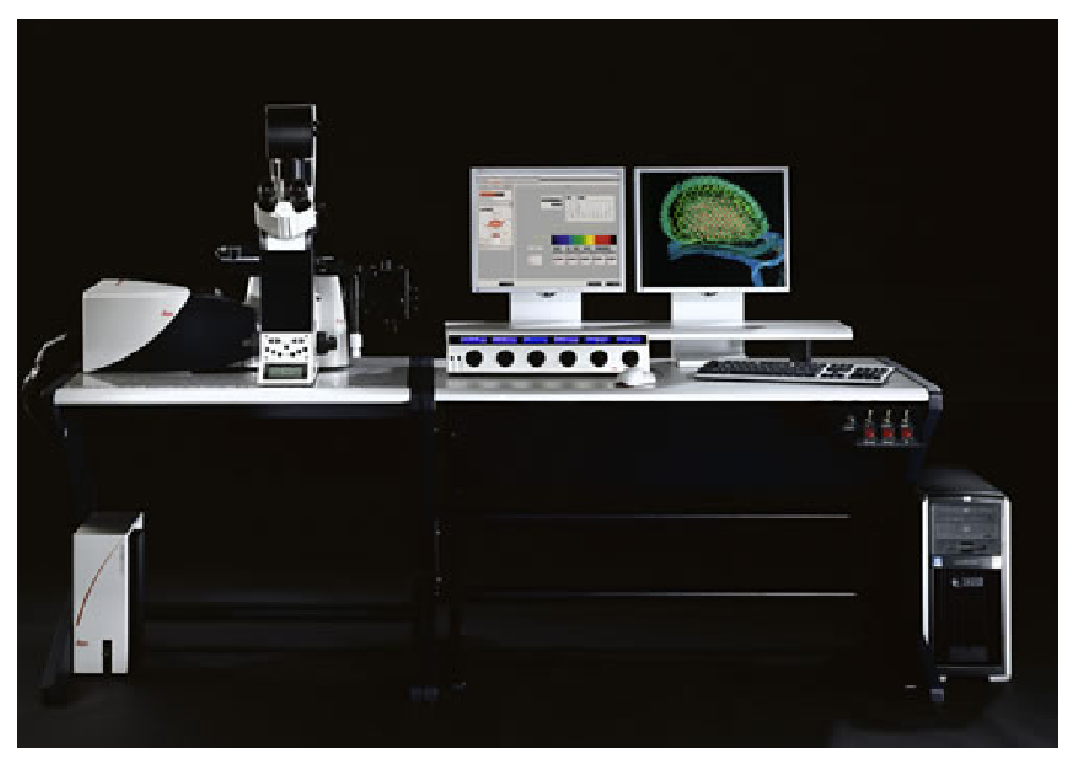
\includegraphics[width=0.5\textwidth]{Leica_SP5}
	\caption{Picture of a Leica SP5 confocal microscope without the temperature control apparatus.}
	\label{fig:Confocal}
\end{figure}


The data was collected on a Leica SP5 confocal microscope, using \unit{532}{\nano\meter} laser excitation. The sample was mounted on a galvano stage, allowing fast scanning in the $Z$ direction (sample is mobile, objective lens does not move). The typical pixel size is \unit{0.298}{\nano\meter} in all three dimensions, leading to a sampling of \unit{11}{pixels} per particle diameter for the most common particle sizes, and still about \unit{8}{pixels} for the smallest particles observed by SEM. The main advantage of using colloids as large as \unit{3}{\micro\meter} is that particles appear as well-defined disks on any 2D slice of the 3D image (see \FigureRef{fig:typical-slice}).

Leica SP5 fast scanner is able to scan with a frequency of \unit{8000}{\hertz}, meaning 8000 lines in a second. A stack of \unit{256}{pixels} in all three dimensions could be acquired in \unit{6}{\second}. On the other end of the spectrum, we were able to program the microscope to take a stack every 30 minutes during a few days. This allows us to follow the dynamics of our colloids through almost three orders of magnitude.

The colloidal suspension was filled into glass capillaries that were then sealed by UV glue. To prevent bleaching of the sample, the centre of the capillary was protected by aluminium foil while the ends were exposed to long wavelength ultra-violet light. We used both square section \unit{500}{\micro\metre} capillary cells and $\unit{100}{\micro\metre}\times\unit{1}{\milli\metre}$ capillary slits. Using an glycerol-immersed long working distance objective lens, we were able to image the whole depth of the slits, and to take data at least \unit{50}{\micro\meter} (\latin{i.e.} $>15\sigma$) far from any wall in the square capillaries.

\begin{figure}
	\centering
	\subfloat[$XY$ slice]{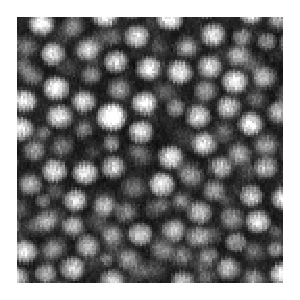
\includegraphics[width=0.4\textwidth]{sliceXY}}\quad
	\subfloat[$XZ$ slice]{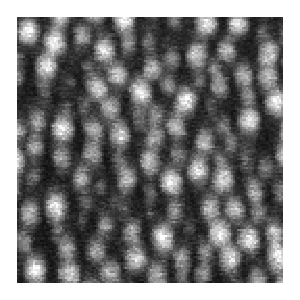
\includegraphics[width=0.4\textwidth]{sliceXZ}}
	\caption{Detail of typical slices of a 3D image of a dense colloidal suspension.}
	\label{fig:typical-slice}
\end{figure}



\subsubsection{Temperature control}
\label{subsubsec:Tcontrol}

Because the sample was mounted on a galvano stage, thus moving precisely at a fast rate, the temperature control apparatus had to be lightweight, with the least inertia possible. On the other hand, we had no need of quick temperature variation. We decided to use only heaters and passive cooling by the air of the room. Then the sample had to be at higher temperature (around \unit{30}{\celsius}) than the room (around \unit{26}{\celsius}).

The sample was lying on a thermostated glass plate (ThermoPlate$\texttrademark$), custom-made by \emph{Tokai Hit Co., Ldt.} to be mounted on the Leica galvano stage. The objective lens was also thermostated because at contact with the sample through glycerol. Provided a temperature difference of at least \unit{2}{\celsius} between the room and the nominal temperature, the deviation from the nominal temperature was no more than \unit{0.1}{\celsius}.

%\newpage
% Create the bibliography right after the text
%\bibliographystyle{ieeetr}
%\bibliography{mathieu}
	\svnidlong
{$LastChangedBy$}
{$LastChangedRevision$}
{$LastChangedDate$}
{$HeadURL$}

\chapter{Particle tracking}
\label{ch:tracking}

In this chapter, we will explain the method used to extract the three dimensional coordinates and trajectories of colloidal particles from the confocal microscope images. This analysis is the basis of the rest of the work in this thesis.

\section{Principle}
More than a century ago, Jean Perrin~\citep{perrin} was measuring coordinates of thousands of Brownian particles on photographic plate with a ruler to prove the sedimentation-diffusion equilibrium. Nowadays, we can program computers to perform the same tedious task. Modern particle tracking by computer image analysis was pioneered by John C. Crocker and David C. Grier~\citep{crocker1996mdv}. Originally a two dimensional process, the algorithm was extended in two ways to treat confocal three-dimensional images. The first method consist in dealing directly with 3D images: each step of the algorithm is implemented in three dimensions~\citep{dinsmore2001tdc}. The second method is to track particles in each 2D slice and then reconstruct a set of coordinate in 3D by another method~\citep{vanblaaderen1995rss, Lu2007, Lu2008}.

In this section, we will describe how does the \ac{CG} algorithm works. In the next section we will detail why and how we re-implemented this algorithm to fit our needs.

\begin{figure}
	\centering
	
\includegraphics[width=0.3\textwidth]{dillute_raw}
	
\includegraphics[width=0.3\textwidth]{dillute_filtered}
	
\includegraphics[width=0.3\textwidth]{dillute_centers}\\
	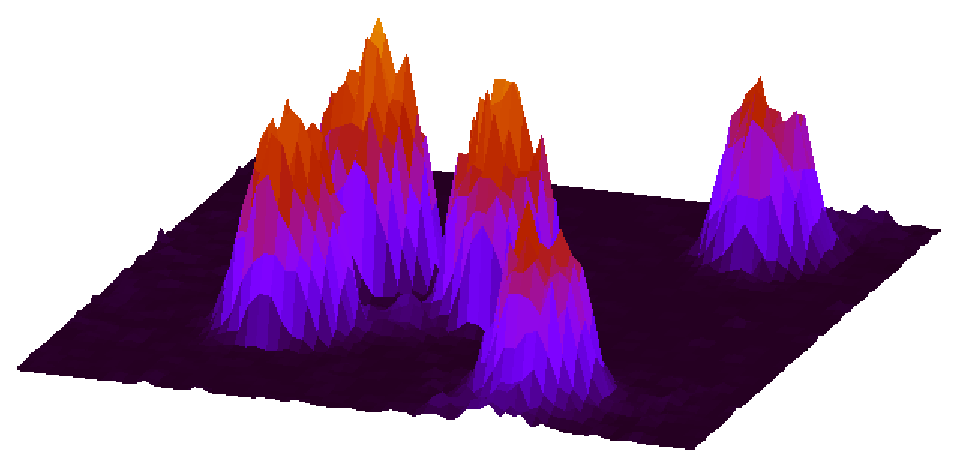
\includegraphics[width=0.3\textwidth]{dillute_raw_gp_raster}
	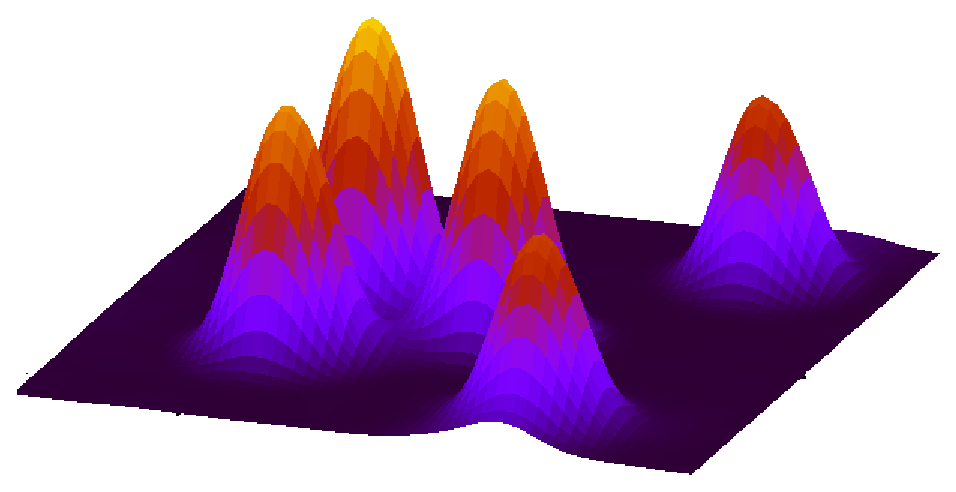
\includegraphics[width=0.3\textwidth]{dillute_filtered_gp_raster}
	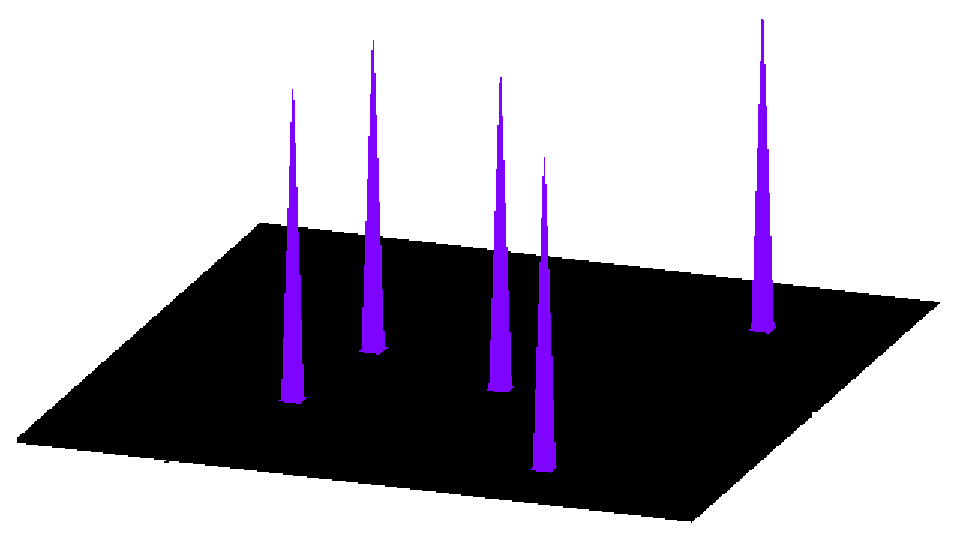
\includegraphics[width=0.3\textwidth]{dillute_centers_gp_raster}
\caption{Schematic Crocker and Grier algorithm in 2D for a dilute sample. The bottom part represent the same image as the top, but with an elevation corresponding to the pixel intensity. Left: Original image. The image noise, at a length scale of a few pixels is particulary apparent in the bottom representation. Middle: Filtered image. The noise has been reduced so that each particle appears as a smooth blob. Right: Tracked centres (low intensity centres were removed).}
\label{fig:track2D}
\end{figure}

The process of the \ac{CG} algorithm is sketched in \FigureRef{fig:track2D} for a 2D image in a simple dilute case. Tracking is done in three steps in each picture (2D or 3D).
\begin{enumerate}
	\item The images are filtered in order to have a Gaussian-like bright blob on a dark background for each particle. 
	\item Potential centres are identified as the pixels that are local intensity maxima (top of the blobs). Most of the time a threshold is needed to discard local maxima due to noise in the (almost) black background.
	\item The precision is refined to sub-pixel by taking the centroid (centre of mass) of the neighbouring pixels.
\end{enumerate}

And finally, the coordinates are linked from time step to time step into trajectories. This last step is not a graphical operation and thus is not included in the tracker. It will be discussed in \SectionRef{sec:time_tracking}.

The \ac{CG} algorithm can seem rough, almost too simple. However it works well with almost identical isotropic objects like spheres. It is known~\citep{crocker1996mdv} to achieve routinely a precision of a tenth of a pixel ($\sim\sigma/100$) in a 2D picture containing hundreds of particles. At the same time, this algorithm has a small set of parameters which allows adaptation to various image quality and experimental conditions. It's main limitation is the polydispersity of the particles. If the particles have too disparate sizes, a multiscale approach~\citep{Adelson1984, Lindeberg1993, OlivoMarin2002, Hinz2005} becomes necessary, but this goes beyond the scope of this thesis. 



\subsection{Image filtering}

\begin{figure}
	\centering
	\subfloat[Not enough blurring]{
\includegraphics[width=0.4\textwidth]{dillute_notblured}}\quad
	\subfloat[Too much blurring]{
\includegraphics[width=0.4\textwidth]{dillute_tooblured}}
	\caption{The same image as in \FigureRef{fig:track2D} with different amount of blurring. Tracked centres are displayed in red.}
	\label{fig:bad_blur}
\end{figure}

Confocal imaging is a trade-off between reducing the thickness of the focal plane and allowing enough light to go through the pinhole. Other constrains, like the need form rapid data acquisition, contribute to make an actual confocal image often noisier than a usual optical microscope image. The noise exists typically on a length scale of a few pixels. Cutting the high frequencies of the image, or equivalently convolving the image with a Gaussian kernel, will remove the noise. The particles will then appear as smooth blobs. The cut-off frequency, or the size of the Gaussian kernel, is crucial (see \FigureRef{fig:bad_blur}). A little bit too much blurring would smear out the smaller particles. Even more blurring and the blobs of the particles begin to merge, leading to ill defined coordinates. Leaving too many high frequencies is not good either, because it allows multiple local maxima per particle, leading to inconsistent tracking.

\begin{figure}
	\centering
	\def\svgwidth{\textwidth}
	\input{track1D.pdf_tex}
	\caption{Schematic 1D picture of the possible distortions of the input image. Top-right: A perfect signal that may correspond to a 1D crystal of slightly polydisperse particles. Each intensity plateau is a particle. Bottom-right: Same signal, but with large scale intensity variation and a small amount of noise. Bottom-left: Same as previous, but with a larger amount of noise. Top-left: Same signals as bottom-left (red) and bottom-right (green) after band-pass filtering. The straight (blue) line is the zero after filtering. Peaks will be detected as particle centres.}
	\label{fig:track1D}
\end{figure}

Image overall intensity can vary quite a lot in space. This can be due to light absorption by the sample, large scale optical aberration and bleaching of the fluorescence. Because the sample absorbs light, the top of the image stack (closer to the objective lens) will be brighter than the bottom (further from the objective lens). One can compensate for this effect at acquisition time by making the gain and the offset of the \ac{CCD} camera $Z$-dependant. At low zoom, one can observe that the centr of a given $XY$ image is brighter than the edges. This effect can be particularly strong in the corners. Furthermore, after some time under the laser, the fluorescent dye beaches. This makes the colloids dimmer. But the colloids that are outside the scanned area do not receive laser light and so stay bright. A problem arises when such unbleached particles diffuse inside the scanned area. Thus, with time, the centre of the scanned area becomes dimmer and dimmer, whereas the edges are populated partly by bright particles from the outside. Both optical aberrations and bleaching cannot be compensated at acquisition time, so a 3D picture out of the scanning confocal microscope is typically heterogeneous in intensity.

Another cause of heterogeneous intensity is intrinsic to the colloids. During the synthesis, a small fraction of the colloids are labelled with much less dye than average; then looking dim under fluorescent microscopy. Conversely, a small fraction of the colloids appear very bright. The later is not a problem, even if the image saturates, but the dim particles are erroneously removed by a threshold that usually distinguish well between particles and noise.

For any of these reasons, it is often useful to remove the low frequencies of the image, except maybe at low density when the background is almost perfectly dark. At low and moderate densities, a high-pass filter has to be tuned carefully if used. If we cut intensity variations at length scales smaller than the distance between two particles, a bright artefact may appear between them. Cut-off length scales of the order of the particle diameter can only be applied at very high densities, were there is no void larger than the particle size. This is only in this latter case that we are able to track a very dim particle surrounded by much brighter particles.

In any case, if the image is band-passed, the two cutting length scales (or frequencies) must be separated by at least a factor 2. If not, the filter will select only a narrow band of frequencies, enhancing random features of the image or even the edges of the particles instead of their centres.

Band pass filtering is often implemented in that way: two copies of the original image are made and blurred by a Gaussian filters of different size. The small-blurred one has the noise removed but brightness heterogeneities remain. The large-blurred one has all the features of the size of the particles erased, keeping only the large scale background intensity variations. The subtraction of the two copies yields the band passed image.

\subsection{Selecting local maxima}

After a good filtering, the selected features of the image (hopefully the particles) are bright and smooth Gaussian blobs on a dark background. Thus there should be one and only one local maxima per particle, on top of the blob. Local maxima are often detected using a dilation filter. Dilation is a morphological filter that assigns to each pixel the maximum brightness of its neighbourhood. This filter was easy to use because it is implemented in in most of the image processing software and libraries (Photoshop, IDL, Intel primitives, etc.). A copy of the filtered image is dilated and compared to the original (filtered) copy. The pixels that have the same value in both versions are the local maxima.

Some local maxima may exist outside any particle. They may be due to noise or to the light coming from an out-of-plane particle because our microscope is diffraction limited (this last effect is drastically reduced if the filtering was done in 3D). Usually, these local maxima have much lower intensities than those corresponding to a particle. They can be easily discarded by a threshold in brightness.

Bad low frequency filtering usually causes many false positive detections. It enhanced dim features far from any particle. It is then impossible to tell them apart by the intensity threshold.

In dense samples, there is no void large enough to host a local maximum. Thresholding is then unnecessary, or even counter-productive because one may discard dim particles.

\subsection{Sub-pixel resolution}

After the detection of local maxima and thresholding, we are be able to assign a pixel to each particle. Our precision is the size of a pixel, typically a tenth of the particle diameter. To go beyond, one can fit a Gaussian on the blob around the local maxima. Equivalently, one can calculate the intensity centroid (centre of mass) of the neighbourhood of the local maxima. This refines precision to a tenth of a pixel, \latin{i.e.} $\sim\sigma/100$.

The pitfall here is to take a too large neighbourhood. If two particles are at contact, optical effects, further enhanced by filtering, will skew the two blobs one towards the other~\citep{Baumgartland2005}. If the neighbourhood used for sub-pixel resolution is too wide, one may catch the influence of neighbouring blobs, thus shifting the coordinates of the particles. This effect is notably strong at the interface between a condensed phase and a gas, for example in the case of colloidal gel. Particles at the interface have neighbours only on one side and their tracked coordinates could then be shifted toward the dense phase.

\section{Implementation}

\subsection{Existing implementations}

The \ac{CG} algorithm was implemented already a few times in various flavours by different people in a few programming languages. Of course, there is the original IDL implementation by John Crocker~\citep{crocker1996mdv}, improved by Eric Weeks. This implementation was cloned in Matlab~\citep{BlairDufesneMatlab, Gao2009} and GDL~\citep{Desmond}. We had also access to the personal C++ implementation of Paddy Royall~\citep{Royall2003}. They all use full 3D localisation method. 

The limiting parameter of full 3D localisation method is the memory of the computer, because the whole 3D image has to be loaded in memory. However in all the existing implementations, the details of the program required at least two high precision copies of the image, \latin{i.e.} two blocks of continuous memory of 8 times the disk space used by the uncompressed image. For example, an uncompressed \unit{8}{\bit} grey scale cubic 3D picture of \unit{256}{pixels} in each direction takes \unit{16}{\mega\byte} on disk. To analyse it with the previous implementation one needs at least two blocks of \unit{128}{\mega\byte}. Such amount of working memory was a challenge a few years ago, but is not a big deal for modern computers. However, simply doubling the size of the image (\unit{512}{pixels} cubic) crosses the limit of \unit{1}{\giga\byte} for each memory block, which is impossible for a MS Windows \unit{32}{\bit} computer.

That is with this limitation in mind that the 2D localisation with 3D reconstruction was implemented first in IDL by van Blaaderen and co-workers~\citep{vanBlaaderen1997} back in 1995 and more recently in C++ by \citet{Lu2007}. 2D tracking is inexpensive in memory and can use the standard filters, algorithms and hardware acceleration of image processing that are almost always implemented in two dimensions. However, the reconstruction step makes assumptions on the intensity profile of a particle in the $Z$ direction. This assumption is fair when the imaging quality is good and the particles monodispersed and of equal brightness. With our slightly polydispersed particles, it was impossible to reach a good precision on the $Z$ coordinate.

All the full 3D implementations are slow, taking typically \unit{10}{\minute} per \unit{256}{pixels} cubic images. They need to perform $O(N^2)$ operations, with $N$ the number of pixels in the image. In addition, interpreted languages like IDL or Matlab are not known for their speed performances.

\subsection{Our implementation}

Because we were planning to investigate heterogeneities of about 10 particle sizes, we wanted to track a large number of particles to reach meaningful statistics. We also wanted a good precision on the position of the particles in three dimensions. And we had a to use colloids with a non-negligible amount of polydispersity. With these constrains, no existing implementation was fitting our needs. Moreover, large data meant slower and slower tracking. So we decided to do our implementation in a compiled language (C++) and to look for both speed and memory optimizations.

Our code is available online~\citep{LeocmachColloids} under the GNU General Public License version 3.0.
\begin{figure}
	\centering
	
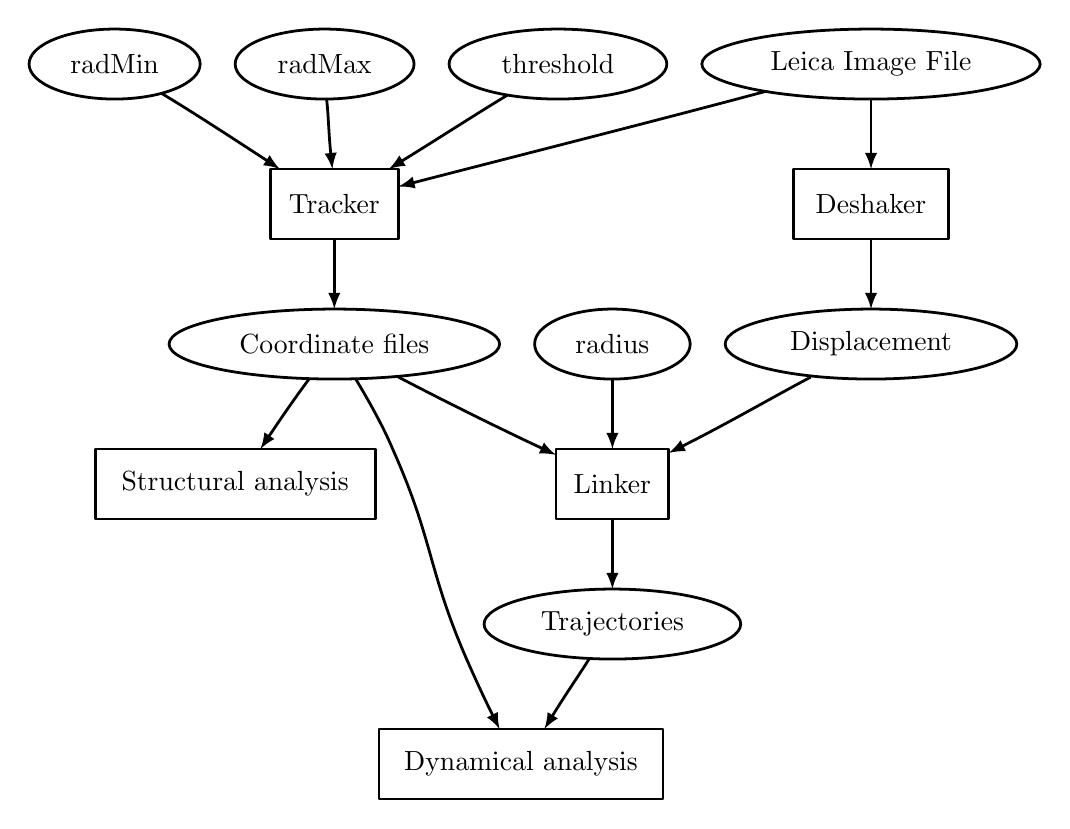
\begin{tikzpicture}[>=latex,line join=bevel,scale=0.7]
  \pgfsetlinewidth{1bp}
%%
\pgfsetcolor{black}
  % Edge: dat_files -> Linker
  \draw [->] (190bp,217bp) .. controls (211bp,206bp) and (239bp,192bp)  .. (271bp,177bp);
  % Edge: threshold -> Tracker
  \draw [->] (246bp,362bp) .. controls (231bp,353bp) and (211bp,340bp)  .. (185bp,324bp);
  % Edge: lif -> Tracker
  \draw [->] (379bp,364bp) .. controls (327bp,350bp) and (248bp,330bp)  .. (190bp,315bp);
  % Edge: dat_files -> Structure
  \draw [->] (144bp,216bp) .. controls (138bp,208bp) and (131bp,198bp)  .. (119bp,180bp);
  % Edge: radMax -> Tracker
  \draw [->] (153bp,360bp) .. controls (154bp,352bp) and (154bp,343bp)  .. (156bp,324bp);
  % Edge: dat_files -> Dynamics
  \draw [->] (168bp,216bp) .. controls (174bp,206bp) and (182bp,192bp)  .. (187bp,180bp) .. controls (208bp,133bp) and (205bp,118bp)  .. (225bp,72bp) .. controls (229bp,63bp) and (233bp,54bp)  .. (242bp,36bp);
  % Edge: lif -> Deshaker
  \draw [->] (433bp,360bp) .. controls (433bp,352bp) and (433bp,343bp)  .. (433bp,324bp);
  % Edge: Tracker -> dat_files
  \draw [->] (157bp,288bp) .. controls (157bp,280bp) and (157bp,271bp)  .. (157bp,252bp);
  % Edge: displ_file -> Linker
  \draw [->] (402bp,217bp) .. controls (383bp,207bp) and (359bp,193bp)  .. (329bp,178bp);
  % Edge: radMin -> Tracker
  \draw [->] (68bp,363bp) .. controls (83bp,354bp) and (103bp,341bp)  .. (129bp,324bp);
  % Edge: radius -> Linker
  \draw [->] (300bp,216bp) .. controls (300bp,208bp) and (300bp,199bp)  .. (300bp,180bp);
  % Edge: Deshaker -> displ_file
  \draw [->] (433bp,288bp) .. controls (433bp,280bp) and (433bp,271bp)  .. (433bp,252bp);
  % Edge: Linker -> traj_file
  \draw [->] (300bp,144bp) .. controls (300bp,136bp) and (300bp,127bp)  .. (300bp,108bp);
  % Edge: traj_file -> Dynamics
  \draw [->] (288bp,72bp) .. controls (283bp,64bp) and (276bp,54bp)  .. (265bp,36bp);
  % Node: radMin
\begin{scope}
  \pgfsetstrokecolor{black}
  \draw (44bp,378bp) ellipse (44bp and 18bp);
  \draw (44bp,378bp) node {radMin};
\end{scope}
  % Node: lif
\begin{scope}
  \pgfsetstrokecolor{black}
  \draw (433bp,378bp) ellipse (87bp and 18bp);
  \draw (433bp,378bp) node {Leica Image File};
\end{scope}
  % Node: displ_file
\begin{scope}
  \pgfsetstrokecolor{black}
  \draw (433bp,234bp) ellipse (75bp and 18bp);
  \draw (433bp,234bp) node {Displacement};
\end{scope}
  % Node: Linker
\begin{scope}
  \pgfsetstrokecolor{black}
  \draw (329bp,180bp) -- (271bp,180bp) -- (271bp,144bp) -- (329bp,144bp) -- cycle;
  \draw (300bp,162bp) node {Linker};
\end{scope}
  % Node: dat_files
\begin{scope}
  \pgfsetstrokecolor{black}
  \draw (157bp,234bp) ellipse (85bp and 18bp);
  \draw (157bp,234bp) node {Coordinate files};
\end{scope}
  % Node: traj_file
\begin{scope}
  \pgfsetstrokecolor{black}
  \draw (300bp,90bp) ellipse (66bp and 18bp);
  \draw (300bp,90bp) node {Trajectories};
\end{scope}
  % Node: Tracker
\begin{scope}
  \pgfsetstrokecolor{black}
  \draw (190bp,324bp) -- (124bp,324bp) -- (124bp,288bp) -- (190bp,288bp) -- cycle;
  \draw (157bp,306bp) node {Tracker};
\end{scope}
  % Node: radius
\begin{scope}
  \pgfsetstrokecolor{black}
  \draw (300bp,234bp) ellipse (40bp and 18bp);
  \draw (300bp,234bp) node {radius};
\end{scope}
  % Node: threshold
\begin{scope}
  \pgfsetstrokecolor{black}
  \draw (272bp,378bp) ellipse (56bp and 18bp);
  \draw (272bp,378bp) node {threshold};
\end{scope}
  % Node: Dynamics
\begin{scope}
  \pgfsetstrokecolor{black}
  \draw (326bp,36bp) -- (180bp,36bp) -- (180bp,0bp) -- (326bp,0bp) -- cycle;
  \draw (253bp,18bp) node {Dynamical analysis};
\end{scope}
  % Node: Deshaker
\begin{scope}
  \pgfsetstrokecolor{black}
  \draw (473bp,324bp) -- (393bp,324bp) -- (393bp,288bp) -- (473bp,288bp) -- cycle;
  \draw (433bp,306bp) node {Deshaker};
\end{scope}
  % Node: Structure
\begin{scope}
  \pgfsetstrokecolor{black}
  \draw (178bp,180bp) -- (34bp,180bp) -- (34bp,144bp) -- (178bp,144bp) -- cycle;
  \draw (106bp,162bp) node {Structural analysis};
\end{scope}
  % Node: radMax
\begin{scope}
  \pgfsetstrokecolor{black}
  \draw (152bp,378bp) ellipse (46bp and 18bp);
  \draw (152bp,378bp) node {radMax};
\end{scope}
%
\end{tikzpicture}


	\caption{End user view of the tracking process.}
	\label{fig:tracking_process}
\end{figure}


\subsubsection{Filtering}

The main innovation is that the image filtering is done in Fourier space. The original image is first Fourier transformed, then multiplied by a band-pass mask and finally inverse transformed. The advantage of this method are both in terms of memory and of speed. For the Fourier transforms, we used the very fast FFTW library~\citep{Frigo2005} that allows
\begin{itemize}
	\item At most $O(N\log N)$ operations, with $N$ the number of pixels. 
	\item In-place real discrete Fourier transforms: only one memory block is needed instead of two. 
	\item Single-precision floating point numbers, sufficient for our purpose and consuming half the memory imprint of the double-precision floating point numbers handled by IDL. The memory block is then only 4 times the size of the uncompressed 3D image.
\end{itemize}

The filter is a 3D binary (boolean pixels, \unit{1}{\bit}) image taking a negligible amount of space in memory. A band pass filter is simply a spherical shell that can be drawn once and then applied on every 3D spectrum of a time series. The multiplication take a negligible number of operations ($O(N)$).

\subsubsection{Local maxima}

A second innovation is to compute the local maxima locally, without dilation filter, thus with only one copy of the image. In addition, the order of local maxima finding and thresholding is reversed: The pixels with an intensity below the threshold are not investigated as potential local maxima. In dilute sample, this little trick can speed up the local maxima detection by a factor 20.

\subsubsection{Conclusion}

At the end of the day, the memory imprint of a \unit{256}{pixels} cubic image is reduced to a block of \unit{64}{\mega\byte} that contains the image or the spectrum and a block of \unit{2}{\mega\byte} for the mask. Tracking is done in less than a second on a Intel i7 computer. A image of \unit{512}{pixels} cubic has a total imprint of \unit{528}{\mega\byte} and is tracked in \unit{4}{\second}. With such performance we were able to cope with the GigaBytes of data needed to study supercooled liquids. In the future, we hope this will allows us to look for rare events, like homogeneous crystal nucleation.

\section{Choosing tracking parameters}

\subsection{The parameters}

\ac{CG} algorithm offers three parameters one can tune to get the best tracking of a given dataset. In our implementation, they are to be set in the following order.
\begin{description}
	\item[$r_{min}$] \hfill \\
		The blurring radius, \latin{i.e.} the inverse of the cut-of frequency of the low-pass filter, \latin{i.e.} the maximum length scale of the noise.
	\item[$r_{max}$] \hfill \\
		The inverse of the cut-of frequency of the high-pass filter, \latin{i.e.} the minimum length scale of background intensity variations. The high-pass filter can be totally disabled.
	\item[threshold] \hfill \\
		The minimum intensity that a local maxima must have to be considered a particle centre.
\end{description}

\subsection{General method}

Usually our goal is to track all the particles, whatever their size, and to minimize the tracking errors.

First, try to track a stack for various values of $r_{min}$ without high-pass filter and with a threshold at one quarter of the intensity scale of the image (if the pixel intensity goes from 0 to 255, choose a threshold of 64). The number $N$ of tracked particles function of the blurring radius $r_{min}$ should decrease steeply and then plateau with a slight decreasing slope. The good $r_{min}$ should be set at the very beginning of the plateau. It corresponds to the degree of blurring where the roughness of the intensity profile of the particles has disappeared, but the smaller particles have not yet been smeared out. For us, this value was typically around 3.

Second, have a try with the last stack of the time series. It is the most bleached 3D image, so the dimmer and the one with the poorest signal to noise ratio. If the sample is dense, try with zero threshold and check that no unwanted centre had appeared. If so, the threshold can be kept at zero. If not, it means that the sample is too dilute. Raise progressively the threshold until no noise is caught in the dark background.

Third, if large brightness inhomogeneities are present in the image that prevents to set an uniform threshold, try to use lower and lower values of $r_{max}$, starting at half the size of the image and dividing by 2 at each step. If the goal is only to correct large scales inhomogeneities, especially if the sample is dilute, don't go too low in $r_{max}$ or artefacts will appear in the voids. 

Fourth, if the sample is very concentrated, without voids and if dim particles are present, $r_{max}$ can be set even lower. Be careful though to always keep $2r_{min} \leq r_{max}$.

This is of course not a definitive user manual but only guidelines valid in the few types of samples we were able to test our tracking program on. There is no better tracker than the human eye, so double-check the tracked coordinates against the original images. For dilute samples, a 3D check like in \FigureRef{fig:compare_image_tracked3D} is efficient. For dense samples a check on a random 2D slice is better.

\begin{figure}
	\centering
	\subfloat
		[3D representation of a confocal image (no filtering). Dark pixels are transparent, bright pixels are opaque with a colour going from blue to red with the intensity.]
		{\label{fig:compare_image_tracked3D_image}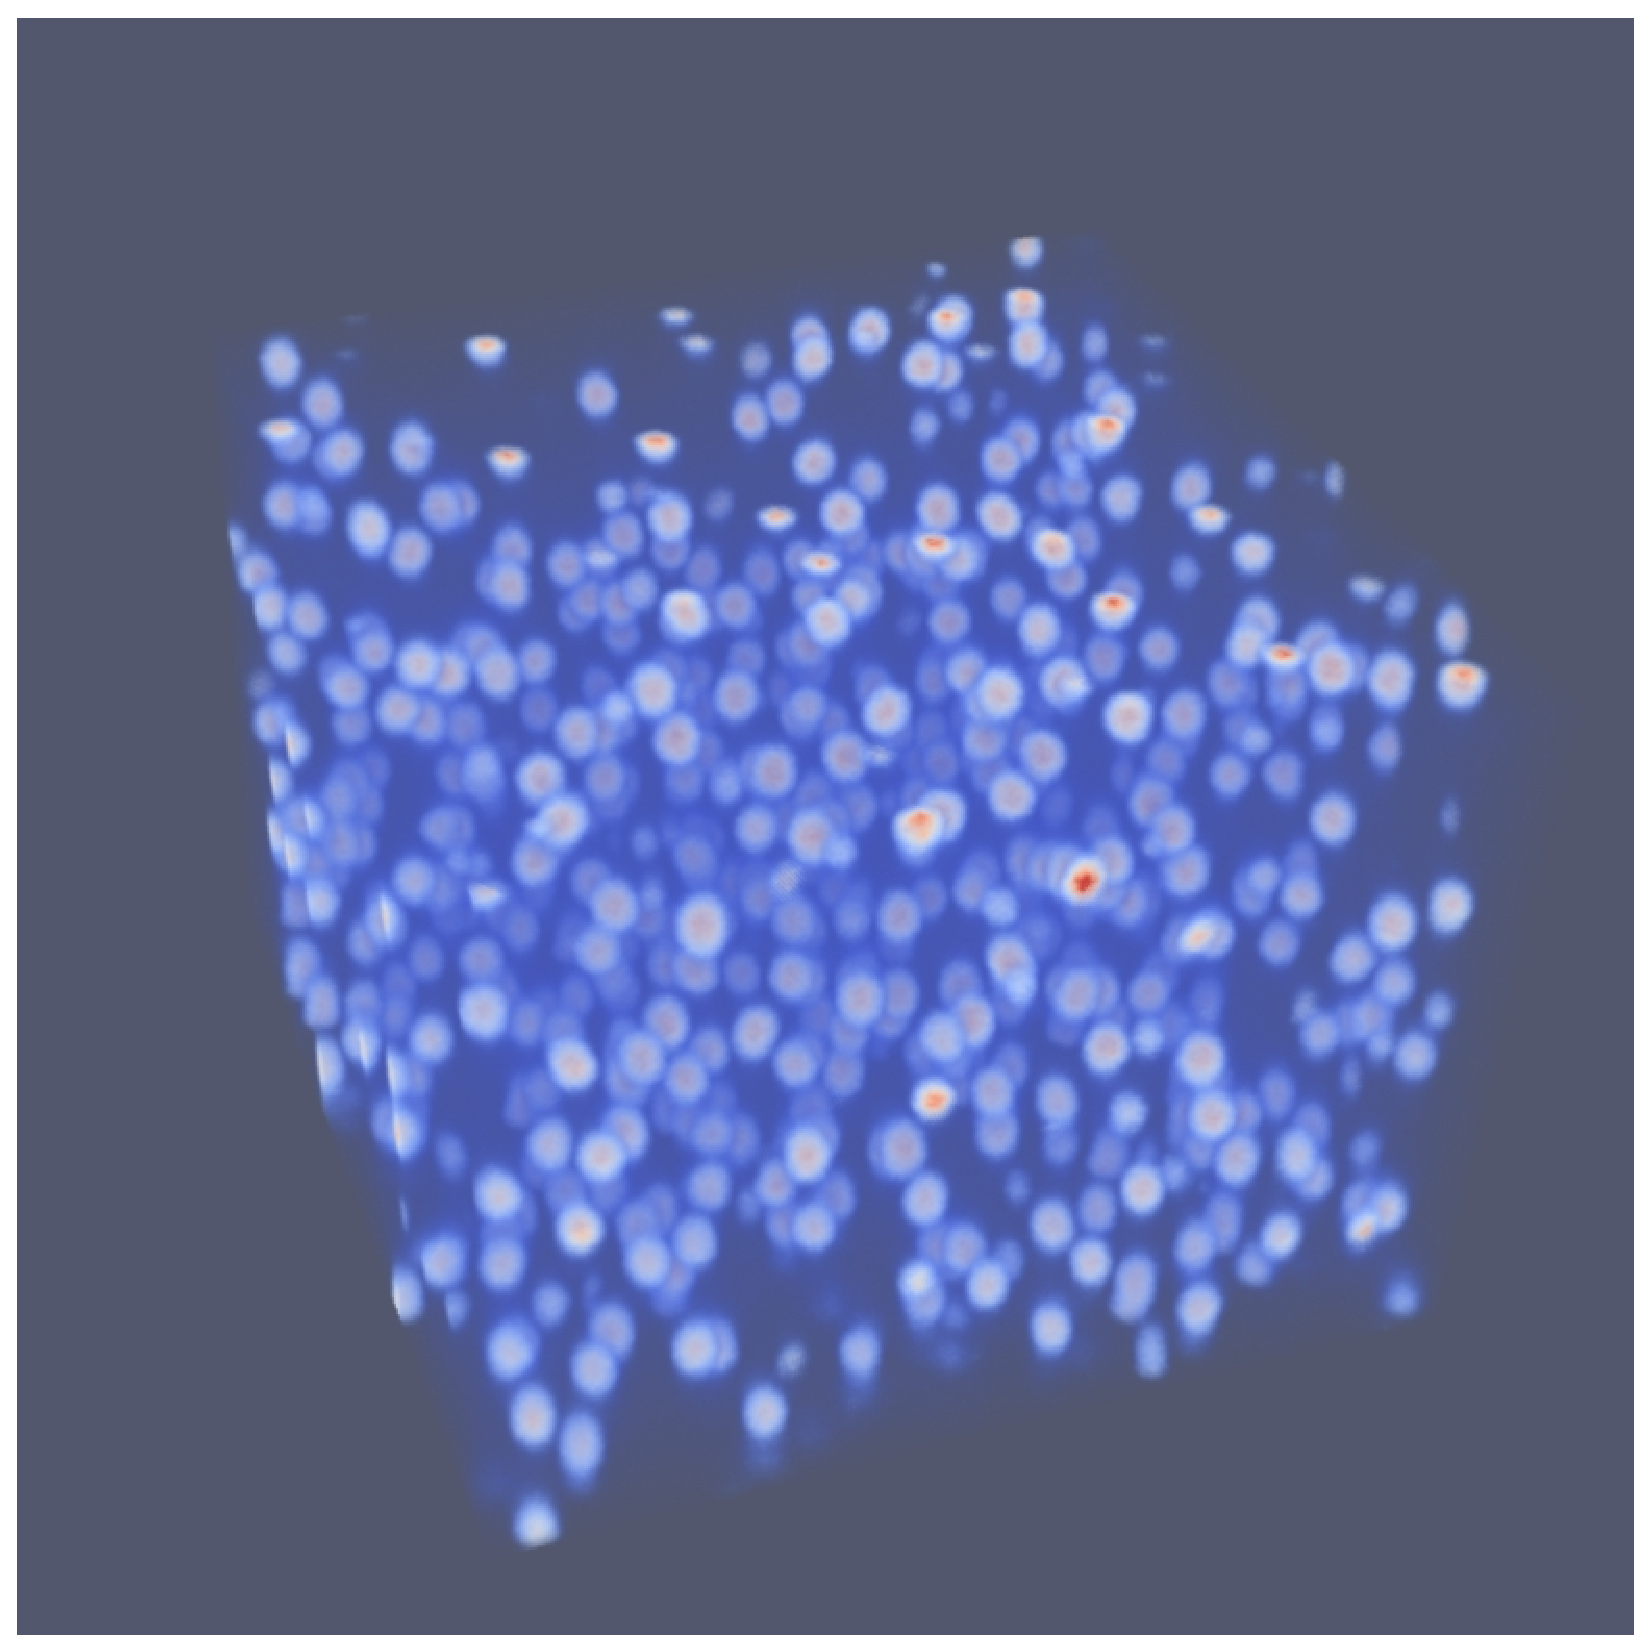
\includegraphics[width=0.45\textwidth]{compare_image_tracked3D_0}}\quad
	\subfloat
		[Plot of the tracked centres. Each sphere has the same diameter (\unit{10}{pixels}). The frame represents the boundary of the picture of the left.]
		{\label{fig:compare_image_tracked3D_plot}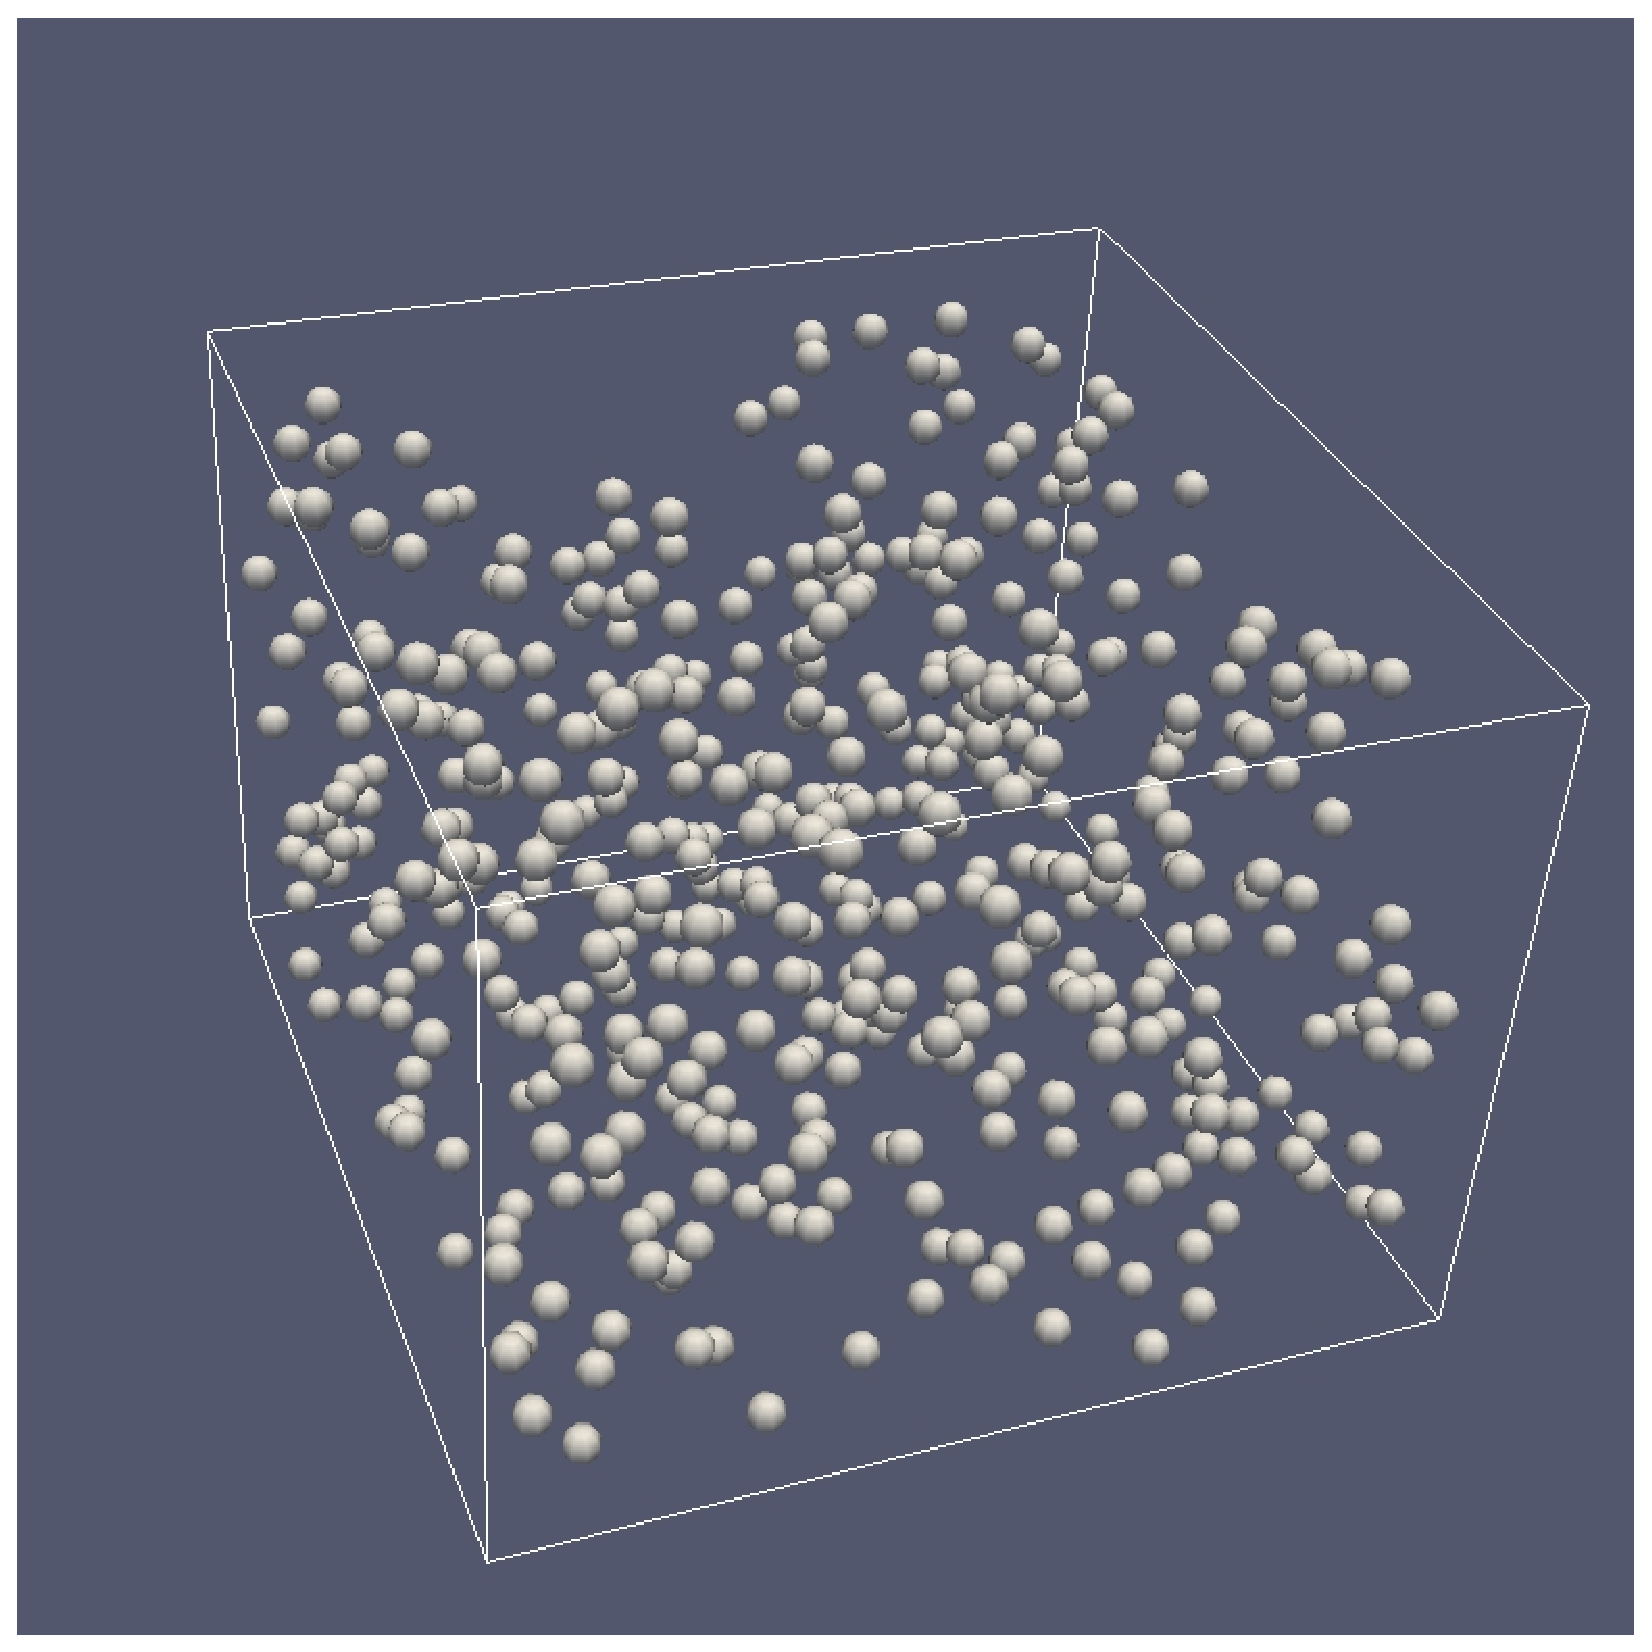
\includegraphics[width=0.45\textwidth]{compare_image_tracked3D_1}}
\end{figure}

\begin{figure}
	\ContinuedFloat
	\centering
	\subfloat
		[Superimposition of \subref{fig:compare_image_tracked3D_image} and \subref{fig:compare_image_tracked3D_plot}]
		{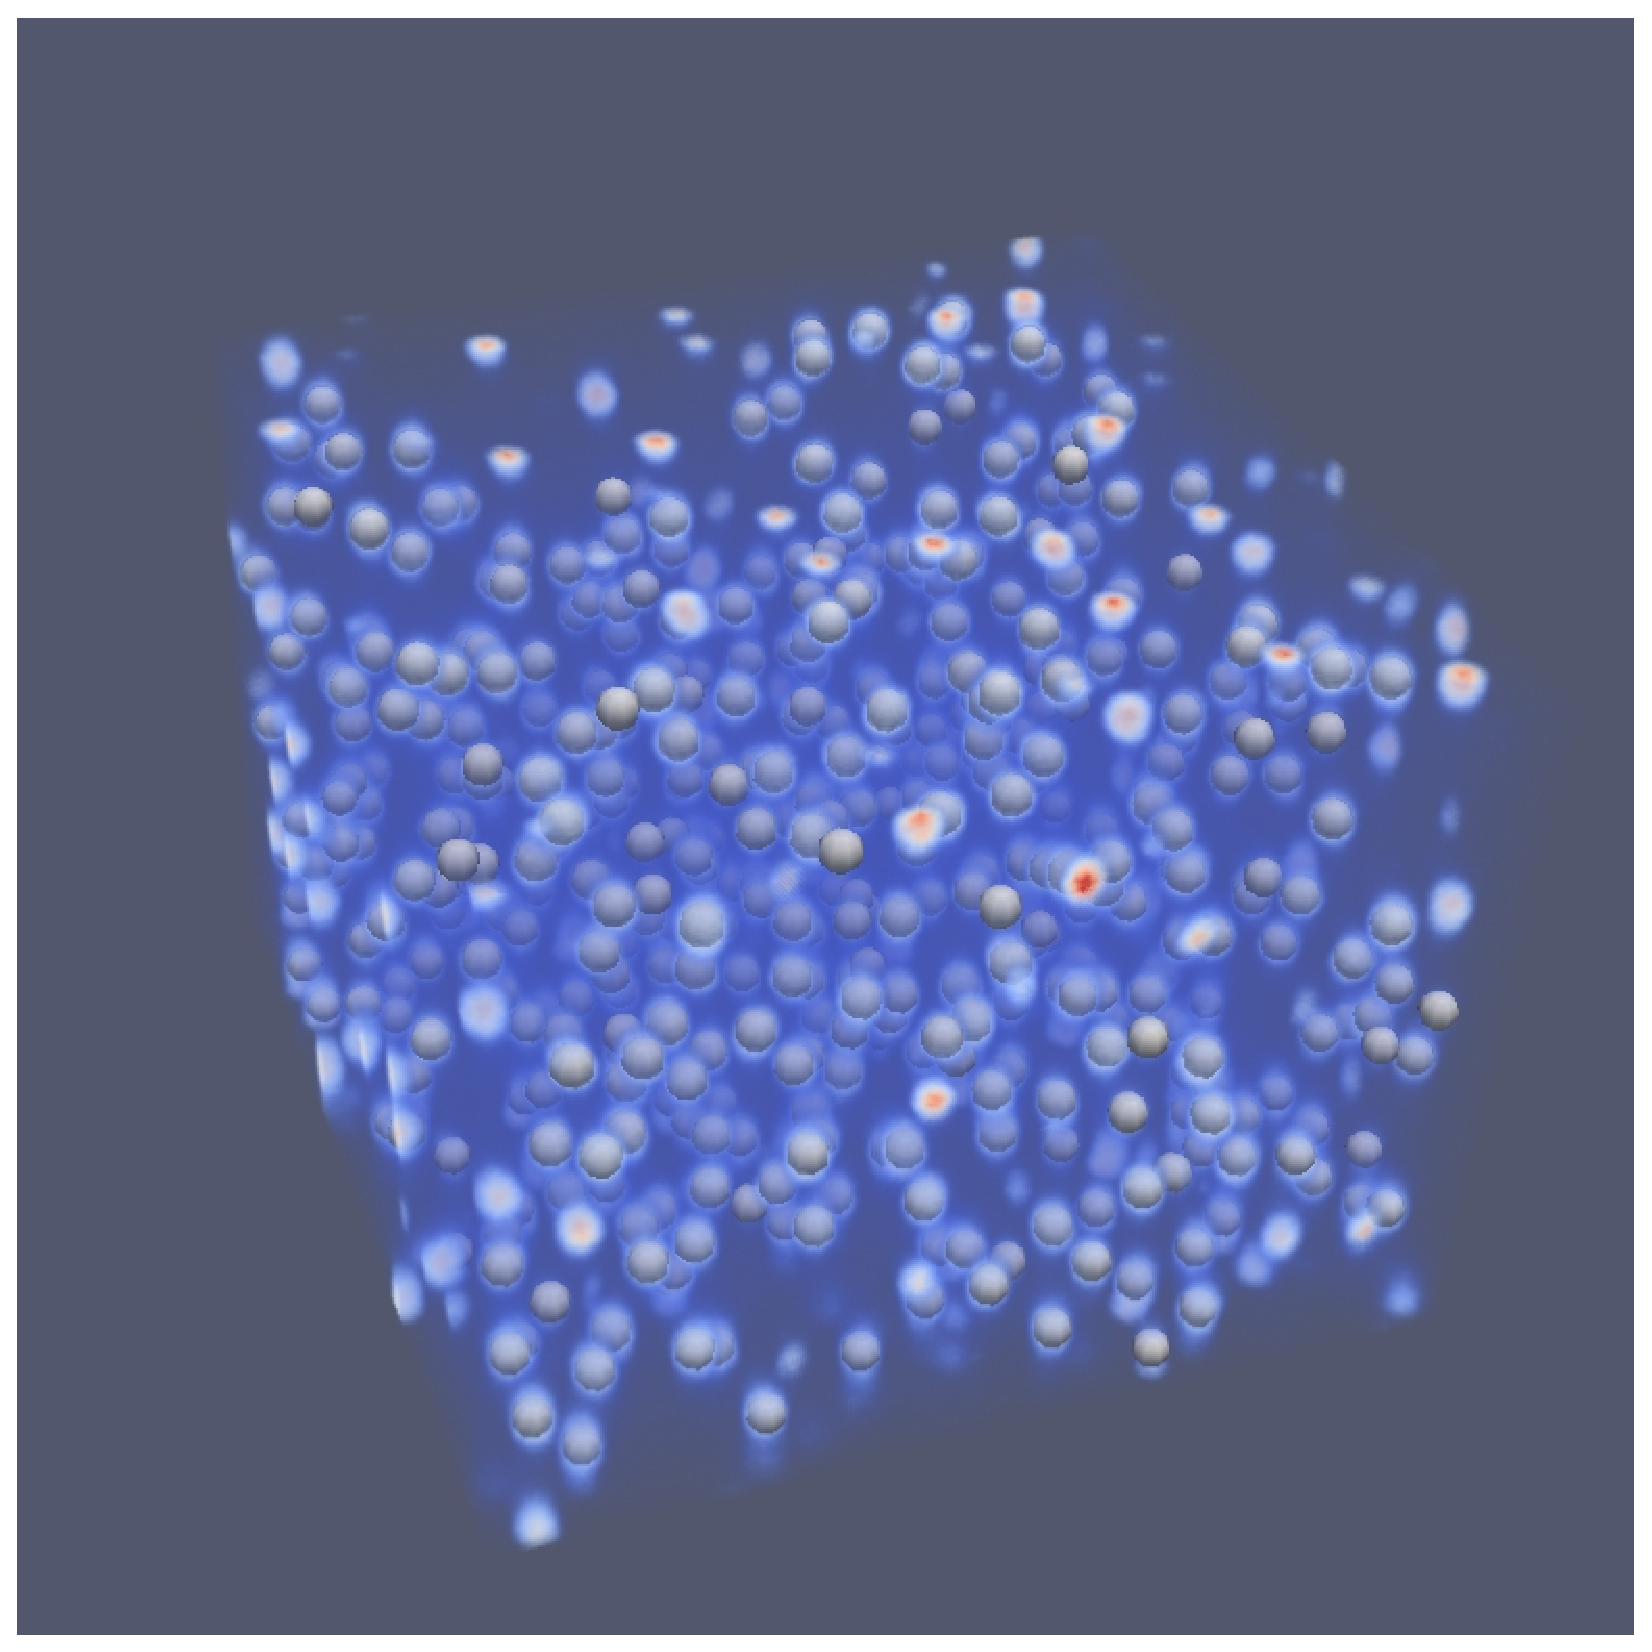
\includegraphics[width=0.8\textwidth]{compare_image_tracked3D_2}}
	\caption{Comparing the original images with the result of our tracking code in a dilute sample (for clarity). The only visible discrepancies are the absence of the particles on the boundary (discarded on purpose) and the size of the smaller particles.}
	\label{fig:compare_image_tracked3D}
\end{figure}

\subsection{Only large particles}

As we have seen in \SectionRef{sec:size_poly}, the colloids we use in experiments can have a non-negligible size polydispersity. A size distribution skewed toward small sizes is very common due to secondary nucleation during the synthesis of \ac{PMMA} particles. If the total number of particles is important to estimate the volume fraction, one can argue that some properties of the system are better caught if the tail of small particles is removed. For instance, structural properties are difficult to extract if the small particles are considered equal to the larger ones, as illustrated by \FigureRef{fig:rdf_tracking}.

\begin{figure}
	\centering
	\input{rdf_size_selection_tracking}
	\caption{Radial distribution function of the same sample tracked in two different ways: with $r_{min}=2.9$~pixels and $r_{max}=5.8$~pixels to catch all particles or with $r_{min}=3.4$~pixels and $r_{max}=30$~pixels to retain only the most common sizes with better precision of the coordinates.}
	\label{fig:rdf_tracking}
\end{figure}

Because our tracking algorithm cannot extract the radii with sufficient precision, we can be tempted to track our images a second time with higher values for both $r_{min}$ and $r_{max}$. Higher $r_{min}$ allows to remove the smallest particles from the filtered image, and removes also more noise leading to drastic improvement in the precision of the coordinates. Higher $r_{max}$ minimizes the filtering artefacts, increases the precision of the coordinates but disables the tracking of dim particles.

Usually we track our images two times: once to track all particles and get the number density and then a second time to get only the most common size range. The difference of number of tracked particles between the two tracking methods can be up to $20\%$ (about $10\sim15\%$ of the volume fraction). We extract the structural information from both and compare them. The small particles drastically alter the \ac{RDF}, smoothing all the peaks as shown in \FigureRef{fig:rdf_tracking}; however the \acl{BOO} (see \SectionRef{sec:boo} and \ChapterRef{ch:structure}) seems to be robust, at least for the most ordered parts of the samples. The results presented in \ChapterRef{ch:structure} corresponds to the tracking of all the sizes.

\section{Time tracking}
\label{sec:time_tracking}

As the output of the tracker, we now have $N(t)$ particle locations at each time $t$, with $N(t) \neq N(t')$ in general. Contrary to a typical simulation output, the number of particle is not constant in time, particles are coming in and out of the field of view, and the particles are truly indistinguishable, with no index to tell them apart. To analyse the dynamics of our system, we need to link the locations into trajectories.

\subsection{Proximity criterion}

The only way to link the location $r_i(t)$ to one of the locations of the next time step $\lbrace r_j(t+1) \rbrace_{j\in N(t+1)}$ is a proximity criterion. We have to suppose that during the unit time interval, any particle moved only a fraction of the typical inter-particular distance. Then, the right $r_j(t+1)$ is the one minimizing the distance $\left\| r_j(t+1) - r_i(t)\right\|$. This is a well-known optimization problem called "all nearest neighbours" that requires $O(N!)$ operations if solved by brute force. The set of possible links forms a network of $N(t)N(t+1)$ bonds.

Crocker and Grier suggested to use only the links shorter than the typical inter-particular distance. The network then reduces to a collection of disconnected sub-networks. Most of the sub-networks contain only one link and are resolved in $N \log N$ operations by most implementations. A sub-network that links $M$ particles to $M$ particles ($M \ll N$) is solved in $O(M!)$ operations at most (often fewer). Some trajectories finish and some trajectories start at each time step.

\subsection{Validity of the hypothesis}

The previous proximity criterion presuppose that any particle moved only a fraction of the typical inter-particular distance $L$ between two consecutive images. A single Brownian particle diffuses its own radius $L$ in the time $\tau_B = \frac{L^2}{2 d D_0}$, with $D_0$ the diffusion coefficient at infinite dilution and $d$ the dimension of space. To allow time tracking of a dilute sample, one need to take a 3D picture every $dt\ll\tau$. With our samples, it means $dt\sim \unit{2}{\second}$.

In dense samples, trajectory linking is paradoxically easier because the diffusion is not free: the dynamics is activated and particles move by hops of a fraction of their diameter. The time interval between two pictures can then be much longer, depending on the volume fraction. A liquid at the limit of supercooling can be tracked with an interval of \unit{5}{\second}. At $\phi=0.55$, \unit{30}{\second} is sufficient. Deeply supercooled liquids allow trajectory linking even with intervals as long as \unit{30}{\minute}.

\subsection{Improvement by spatial query}

Rather than calculating the length of all the possible links, we used the spatial queries described in \SectionRef{sec:spatial_query} to select quickly the possible links. With this method, the reduced network is constructed in $O(N(t)\log N(t+1)$ operations and contains only $P=n N(t)$ potential links, with $1\leq n \leq 2$.

\subsection{Keep only the shortest}

We can then sort the potential links by increasing length. This is done in $O(P\log P)$ operations. By definition, the shortest potential link minimizes the proximity criterion: it is a good link. Let us note $p$ and $q$ the locations of the beginning (time $t$) and the end (time $t+1$) of this link. If there exist other potential links starting from $p$ or ending at $q$, they are longer than our link $(p, q)$, so they are not good links, so we discard them. The remaining links are still sorted by increasing length and the shortest is a good link. We continue this procedure until no potential link is left. At the end of this algorithm, we have selected the subset of potential links that minimizes the proximity criterion. All the trajectories that have not found a location at $t+1$ finish. All locations that are not linked to an existing trajectory are the starting point of a new trajectory.

The key of the efficiency of this algorithm is the time to find and discard all the links that contains $p$ or $q$. Brute force searching takes $N_{link}$ comparisons for $p$ and the same for $q$, so a total cost of $O(P \times N)$. To find them more quickly, we can index the set of potential links in both $p$ and $q$, independently. That reduces the searching cost to $O(P\log P)$ operations.

\subsection{Implementation using a bidirectional map}

Maintaining two indices on a constantly updating set of objects can be a pain for a non-professional programmer and thus terribly error prone. Thankfully, the boost libraries~\citep{boost} provides a structure called bidirectional map, inspired by \ac{RDMS}, that does exactly the work needed here. It is a set of pairs $(p,q)$, indexed by both keys. This structure enforces the uniqueness of each $p$ and each $q$. That is to say that, if one wants to insert a pair whose first element is already the first element of another pair, then the insertion is silently ignored. This is the same for the second element. Checking the uniqueness before insertion costs $O(\log G)$ with $G \leq N$ the number of good links already inserted.

With the bidirectional map, the linking algorithm becomes very simple. Once the potential links are sorted by increasing length ($O(P \log P)$), they are inserted one by one into the bidirectional map. Bad links are automatically not inserted. Each tentative insertion costs $O(\log G)$, for a total of $O(P \log G)$. New trajectories are started if needed. To sum up, the linking operation behaves at most like $O(N\log N)$.

\section{Other improvements}

\subsection{Reading Leica files}

Thanks to the open-source software community, we could find and integrate into our tracking software a piece of code~\citep{kankaanpaa2006bioimagexd} that reads \ac{LIF}, the (proprietary, undocumented) output format of our microscope. Before, the data needed to be exported as 2D TIFF images (one per $XY$ slice) and then read back into the tracking code. This step was consuming hours of disk I/O time for nothing.

\subsection{Deshaking}

When the time interval between image acquisition is set to more than \unit{1}{\minute}, some overall displacement of the sample appears between time steps. The amount of displacement can be larger than the size of the particles, breaking completely the linking hypothesis. This very annoying effect remained a mystery for weeks. We first thought it was due to flow in the sample, so we doubled-checked the glue sealing the capillary and investigated the temperature control.The seismic activity of Japan, the walking of people nearby or the air flux of the air conditioner could not be accused because our microscope is standing on a vibration isolation table and the displacement was periodic with a period of a few minutes. Finally, we discovered that this displacement was due to the automatic realignment of the microscope stage that is impossible to disable.

We had to find a way to get rid of the global drift by post-processing the data. This is actually a very active field of research in applied optics and is called "digital image stabilization" on commercial digital video cameras. In our case (two almost identical but translated images), it is rather called "image registration". This type of method was developed originally to register a set of satellite pictures into a larger map~\citep{Brown1992}. The simpler and most robust method is the phase correlation alignment method~\citep{kuglin1975phase} based on the Fourier shift theorem. 

Given two input images $g_a$ and $g_b$, we apply a window function (\latin{e.g.}, a Hamming window) on both images to reduce edge effects. Then, we calculate the discrete 2D Fourier transform of both images:
\begin{align}
\mathbf{G}_a = \mathcal{F}\{g_a\} \\
\mathbf{G}_b = \mathcal{F}\{g_b\}
\end{align}
and calculate the cross-power spectrum $R$ and its inverse Fourier transform, the the normalized cross-correlation $r$:
\begin{align}
    R = \frac{ \mathbf{G}_a \mathbf{G}_b^*}{\left\|\mathbf{G}_a \mathbf{G}_b^*\right\|} \\
    r = \mathcal{F}^{-1}\{R\} 
\end{align}

If the two pictures are actually not too different one from the other, and that the images present no periodic patterns, then the result is a noisy dark background with a single bright peak. The position of this peak gives the translation between the two pictures.

Rather than actually translate the pictures, the particle localization is done on the original image. However, before linking trajectories the coordinates are translated to correct the overall displacement (see \FigureRef{fig:tracking_process}).

Recently~\citep{Besseling2009}, this method was used to track non-uniform flows of particles. The phase correlation alignment method was applied on every slice to reconstruct a complex shear profile. Because our global displacement was uniform in the $XY$ plane, we apply this method in 2D only on the the middle slice of the 3D stack.
%\newpage
% Create the bibliography right after the text
%\bibliographystyle{ieeetr}
%\bibliography{mathieu}
	\svnidlong
{$LastChangedBy$}
{$LastChangedRevision$}
{$LastChangedDate$}
{$HeadURL$}

\chapter{Local structure identification in real space}
\label{ch:structure_id}
%Author: \svnauthor; Revision: \svnrev; Last changed on: \svndate; URL: \url{\svnkw{HeadURL}}
% Create a new 1st level heading
\section{Introduction}
\subsection{Crystallography}

From the end of the 18th century, natural scientists rediscovered the atoms invented by the ancients. In parallel, they began to explore the structure of condensed matter, starting by crystals. Rene-Just Hauy~\citep{Hauy1784} imagined that the peculiar proportions and angles of crystals were due to the shape of their elementary building bricks. Gabriel Delafosse~\citep{Delafosse1840} made the essential distinction between an atom and this crystal brick: the brick is an elementary structure made of atoms (or molecules). Auguste Bravais~\citep{Bravais1866} made the inventory of the 14 possible crystal lattices, corresponding to the 32 point symmetry groups.

The idea that crystals are periodically ordered was amazingly successful. Crystallographers were able to predict all the characteristic angles that could appear between the facets of crystals of any given type. With the discovery of x-ray diffraction (see \SectionRef{Diffraction}) in crystals by Max von Laue~\citep{Laue1912} in 1912 and the subsequent development of x-ray crystallography by William H. and William L. Bragg~\citep{bragg1965crystalline} the theory of crystallography received an unequivocal stamp of approval.

\begin{figure}
	\centering
	\subfloat[\acs{FCC}]{\label{fig:FCC}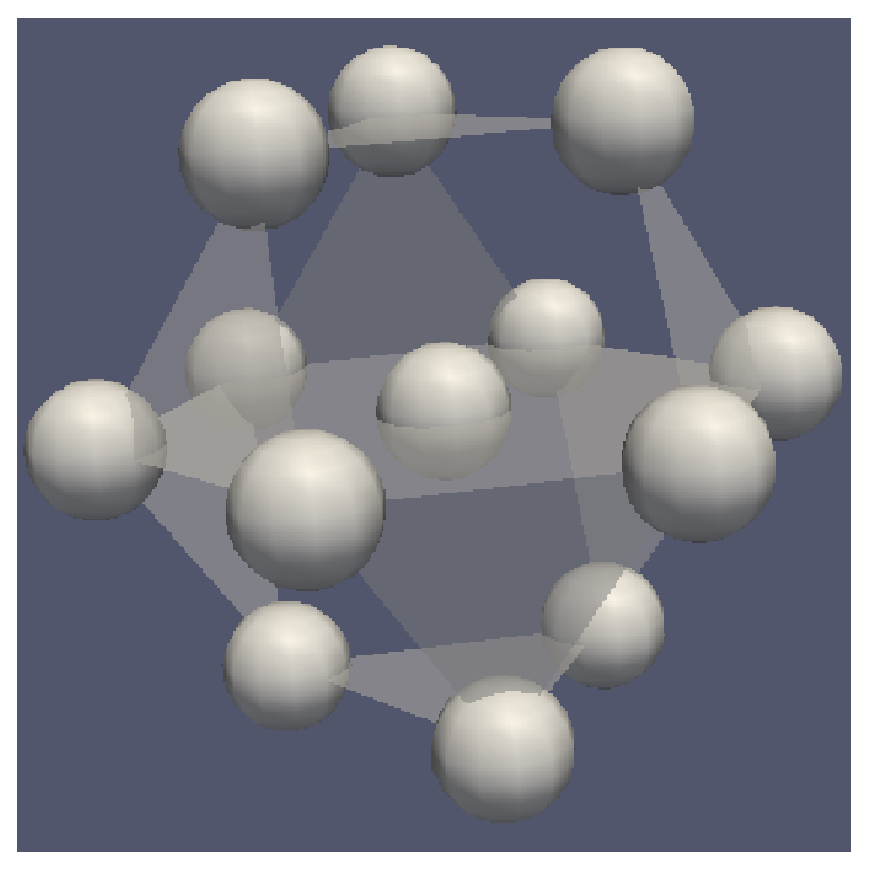
\includegraphics[width=0.3\textwidth]{fcc_13}}
	\subfloat[\acs{HCP}]{\label{fig:HCP}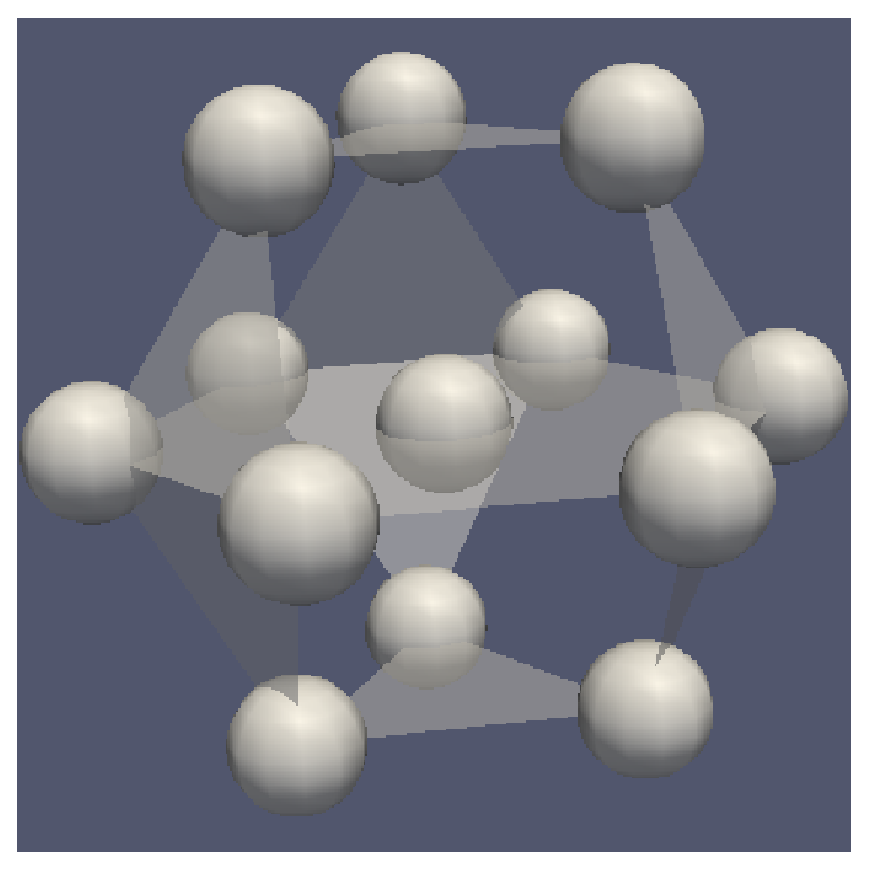
\includegraphics[width=0.3\textwidth]{hcp_13}}
	\subfloat[Icosahedron]{\label{fig:ico}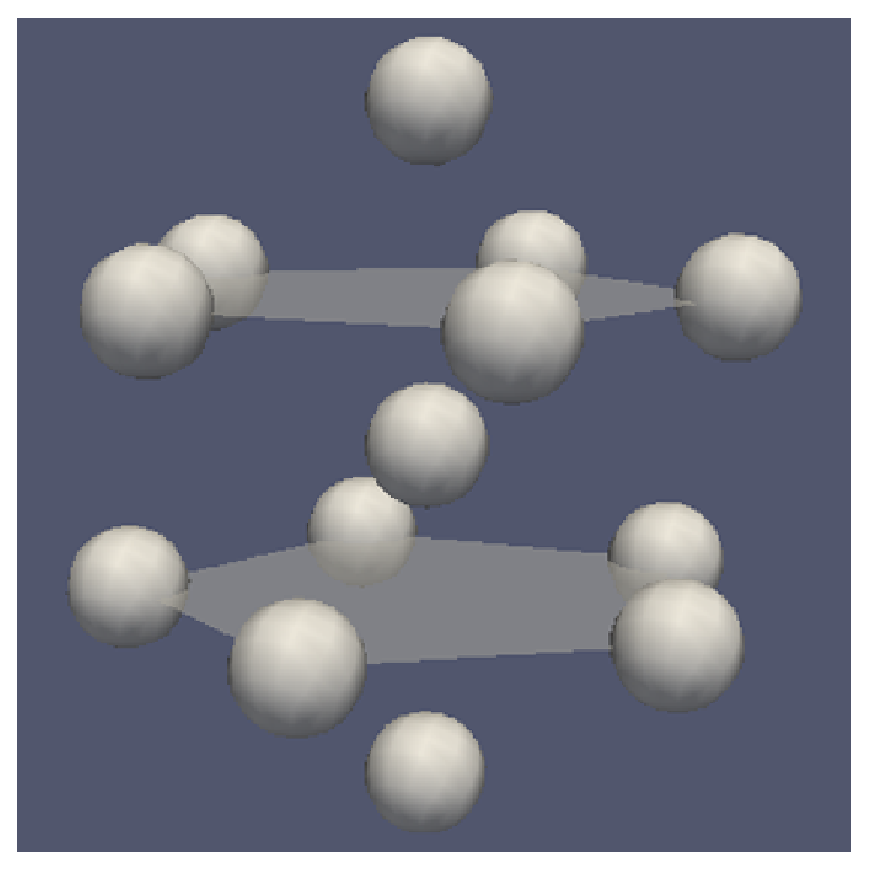
\includegraphics[width=0.3\textwidth]{ico_13}}
	\caption{The three possible clusters made of 12 spheres in contact with a central sphere.}
	\label{fig:basicClusters}
\end{figure}

\begin{figure}
	\ContinuedFloat
	\centering
	\subfloat[9 particles \acs{BCC}]{\label{fig:BCC9}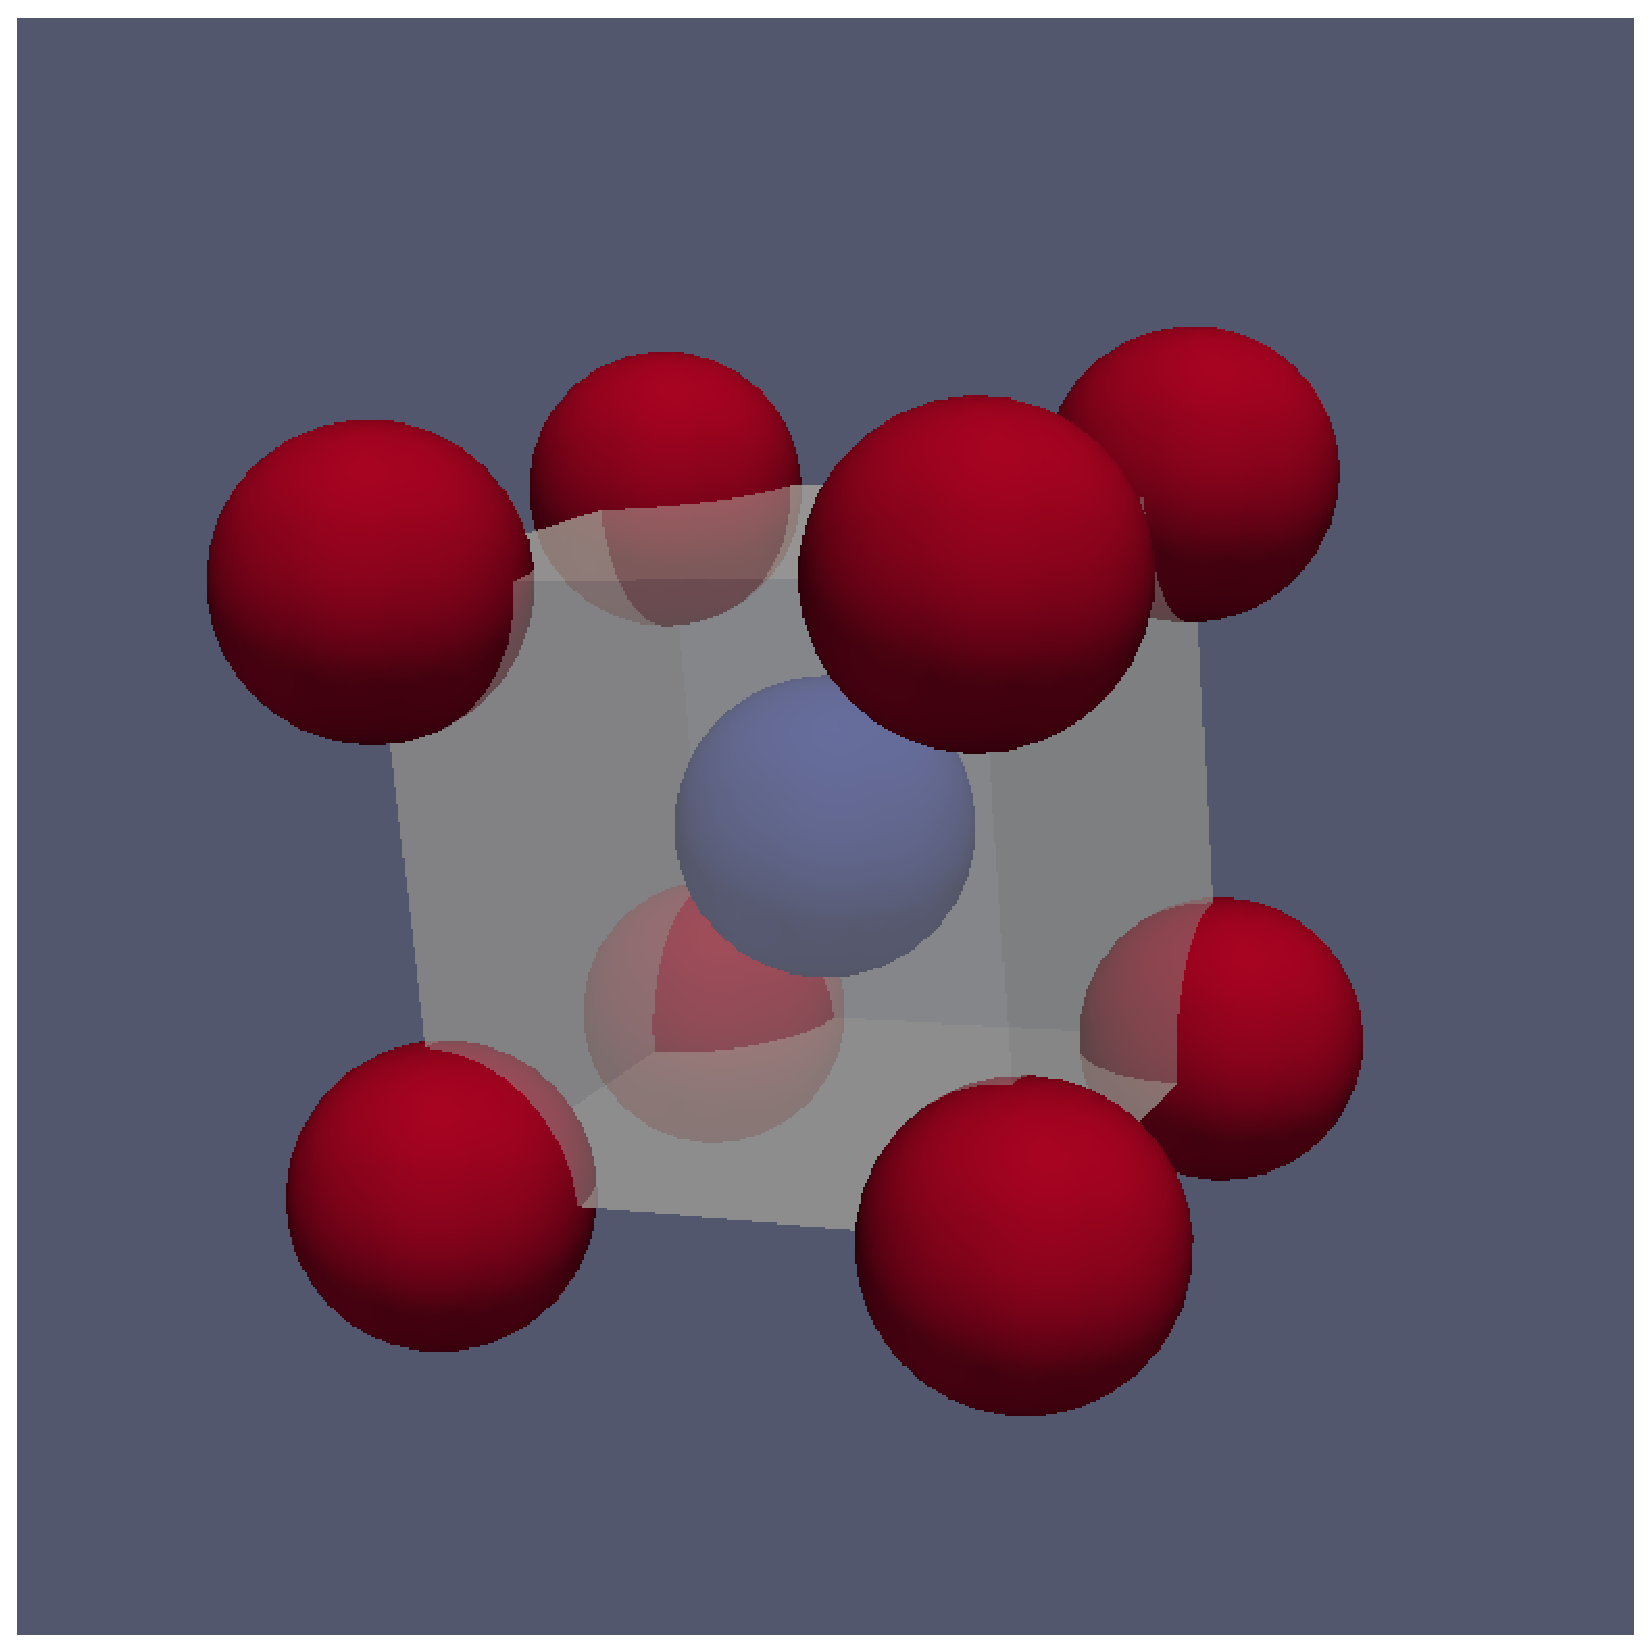
\includegraphics[width=0.3\textwidth]{bcc_9}}
	\subfloat[15 particles \acs{BCC}]{\label{fig:BCC15}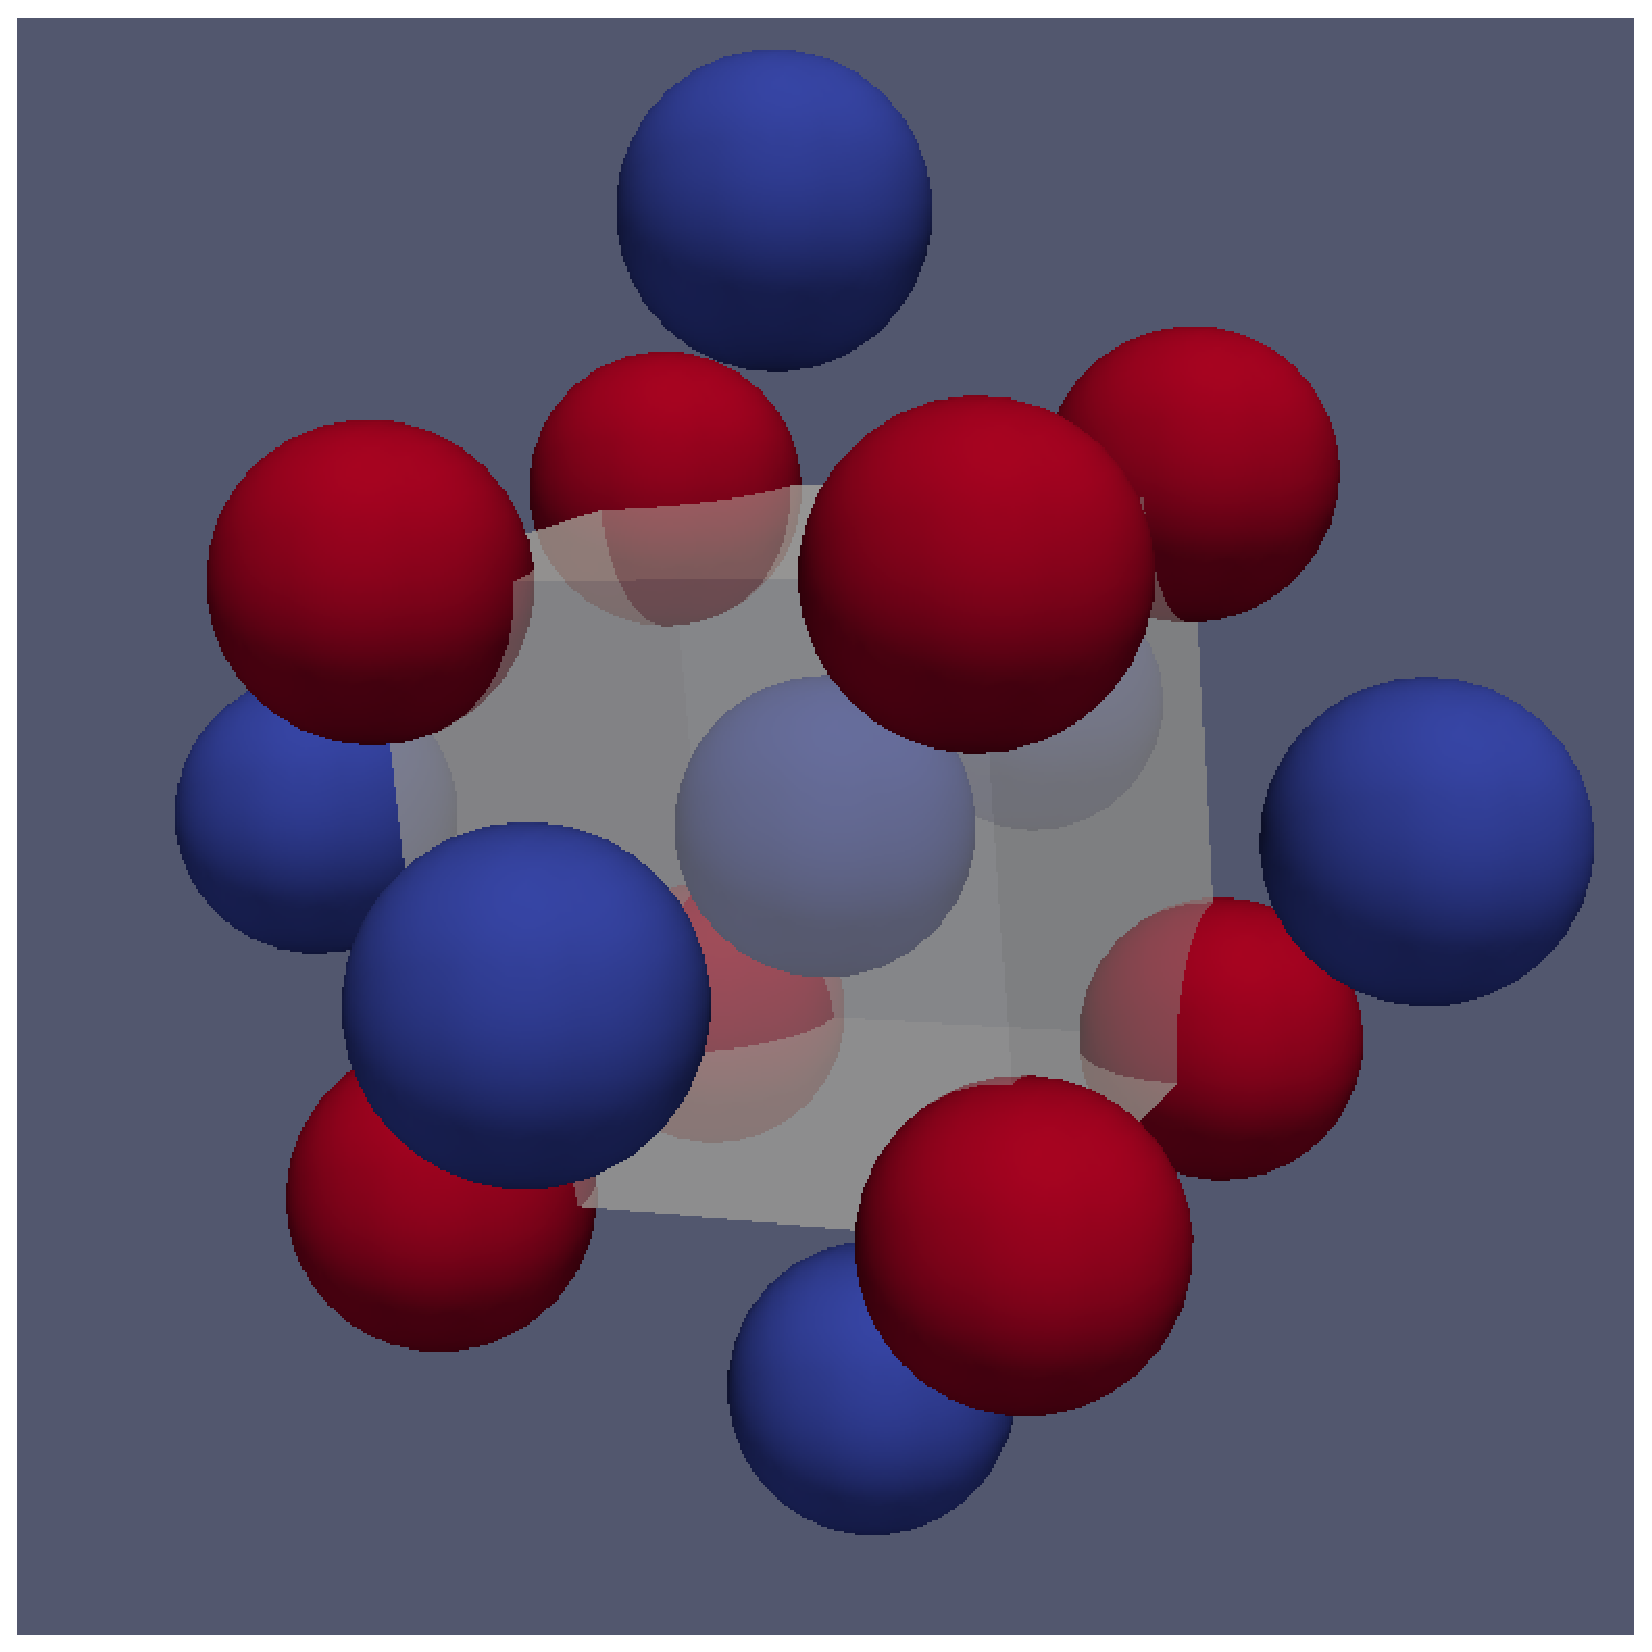
\includegraphics[width=0.3\textwidth]{bcc_15}}
	\subfloat[Dodecahedron]{\label{fig:dodecahedron}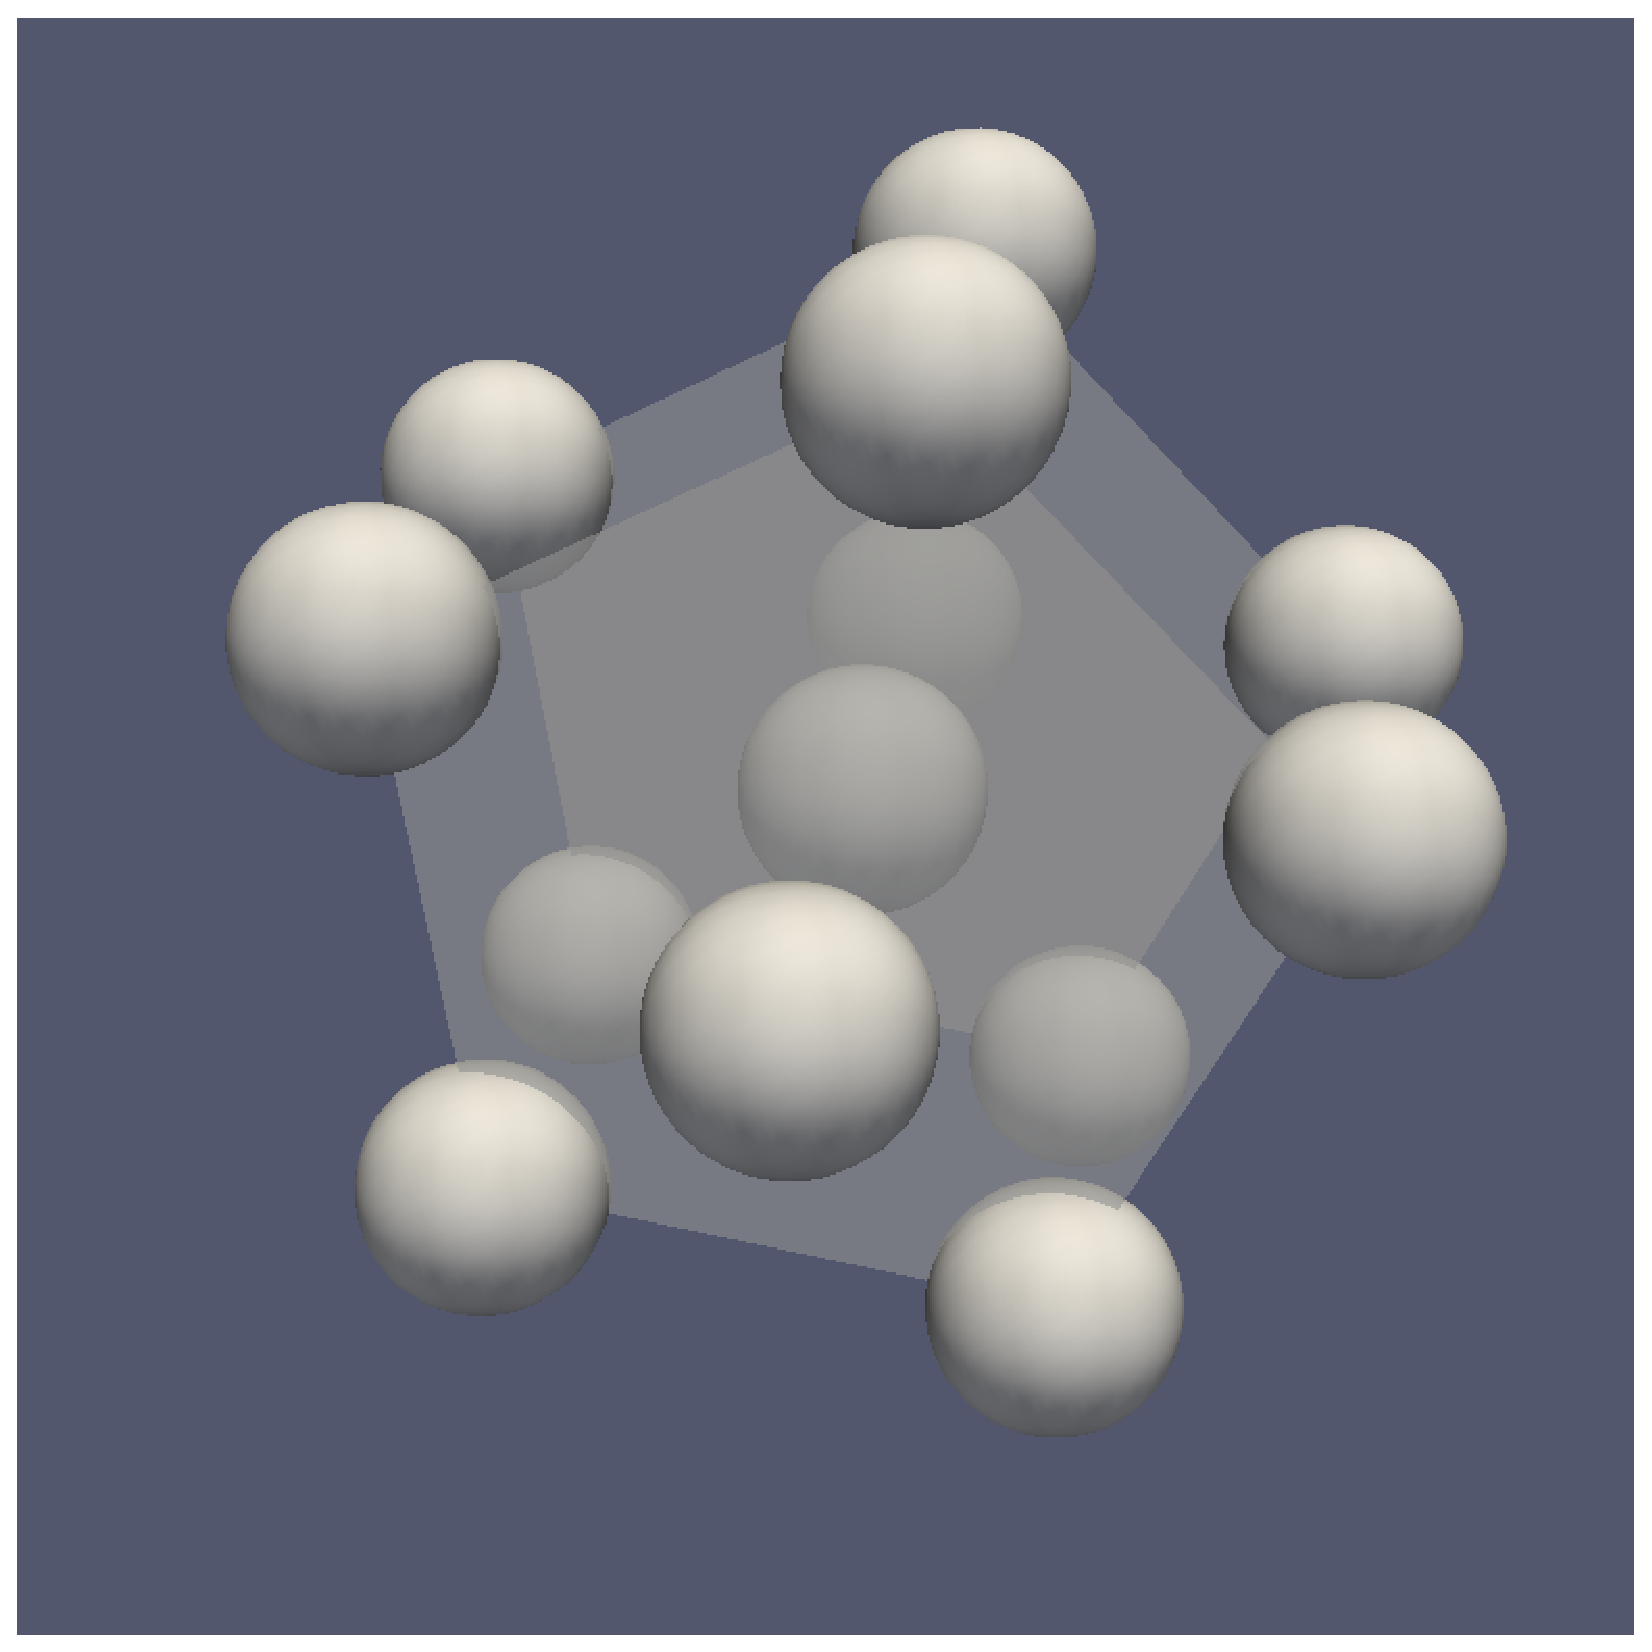
\includegraphics[width=0.3\textwidth]{dodec_13}}
	\caption{Other simple clusters.}
	\label{fig:other_clusters}
\end{figure}

\subsection{Non-crystalline condensed matter}

Disordered structures are not random structures. There is still order in an amorphous or a liquid material. The main point is the lack of periodicity which was the reference for the definition of the order. Periodic crystalline order supposes three types of order: local order, positional order and orientational order. Quasi-crystals, discovered in the 1980's~\citep{Shechtman1984} have a clear orientational order (\FigureRef{fig:diffraction}) but without any periodicity (positional order). In amorphous or liquid structures only the local order remains.

In the metallic structure with isotropic interaction, the local order is similar to the one obtained in a packing of soft balls. All particles have roughly 12 neighbours. But has observed by Frank~\citep{Frank1952}, the 13 particles icosahedral arrangement (see \FigureRef{fig:ico}), incompatible with space tiling, has a significantly lower energy than the \ac{FCC} (\FigureRef{fig:FCC}) and \ac{HCP} (\FigureRef{fig:HCP}) arrangement, at least for the simple Lennard-Jones pair potential. This is a very simple example of local order. In covalent structures like silicon there are oriented interactions leading to the tetracoordinated local order which is a more complex example, but in all cases a local order can be defined. So, a dense phase cannot be completely disordered like a gas, and this has very important consequences for mechanical and physical properties (heat conduction, phase transition, etc.).

\subsection{Diffraction}
\label{Diffraction}

\begin{figure}
	\centering
	\subfloat[Schematic principle of X-ray diffraction.]{\label{fig:diffraction_sketch}\def\svgwidth{0.5\textwidth}\input{xray.pdf_tex}}
	\subfloat[Typical diffraction diagram of a quasicrystal.]{\label{fig:quasiX}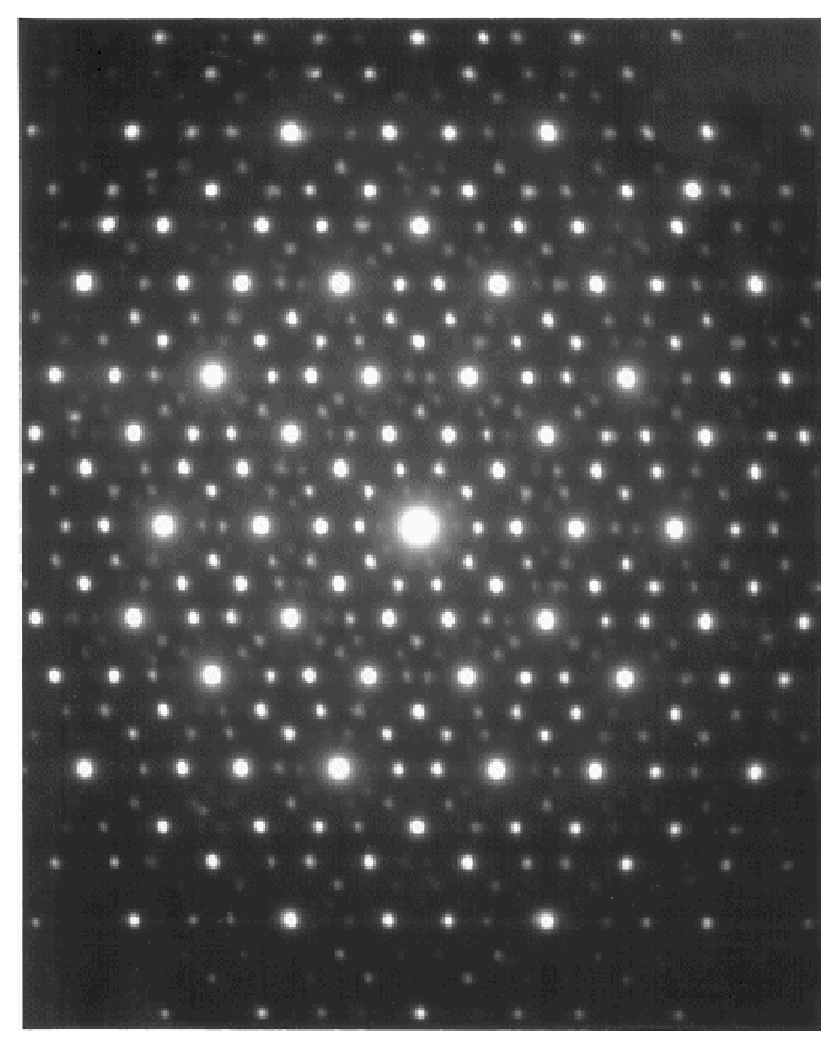
\includegraphics[width=0.4\textwidth]{diffraction_quasiX}}
	\caption{The diffraction patterns indicate \subref{fig:diffraction_sketch}~6-fold and \subref{fig:quasiX}~5-fold or 10-fold rotational symmetry.}
	\label{fig:diffraction}
\end{figure}

Since 1912 and the experiments of Max von Laue~\citep{Laue1912}, the structure of condensed matter can be explored by diffraction. A beam of X-rays, neutron or electrons has a sufficiently short wavelength to probe the material at the atomic scale. The diffracted beam cannot be focused to produce images, so the sample structure must be reconstructed from the diffraction pattern. Sharp features in the diffraction pattern arise from periodic, repeating structure in the sample, which are often very strong due to coherent reflection of many photons from many regularly spaced instances of similar structure, while non-periodic components of the structure result in diffuse (and usually weak) diffraction features.

Conventional diffraction techniques only allow to extract structural information averaged over the illuminated sample area. If a structure is smaller than this area, its signature is averaged out by the surrounding incoherent structures~\citep{Wochner2009}.

Because of their highly ordered and repetitive structure, crystals give diffraction patterns of sharp Bragg reflection spots (\FigureRef{fig:diffraction}). However, amorphous or soft materials are much more difficult to analyse. Non-periodic local structures - sometime important for the physics and the mechanical properties of the material - are often hidden by the configurational averaging.

\subsection{Granular matter, colloids and simulation}

A way to study medium range or local structures by diffraction is to use larger particles, scaling up everything except the illuminated area. So that local structures size become comparable to the illuminated area.

For example, one can use colloids, \latin{i.e.} \unit{100}{\nano\meter} to a few microns objects subject to Brownian motion and thus exploring space like atoms. Colloids can behave as hard spheres or can be given interaction potentials: purely repulsive due to charges, or attractive due to the depletion interaction. They are able to form various state of matter like gas, liquids, crystals, gels and glass. Colloids are model atoms.

With the larger colloids, larger than the wavelength of visible light, direct optical imaging is possible. Using confocal microscopy, it is even possible to track the coordinates of tens of thousand particles in three dimensions (see \ChapterRef{ch:tracking}). The accessible data is then real space data, not diffraction spectrum in Fourier space.

Another possible model atom system is granular matter: sand, steel balls or rice seeds, etc. When granular matter is fed energy (shaking, periodic shear, etc.), the particles explore space almost like atoms. They can constitute fluids, solids (amorphous or crystal). Gains also can be tracked in real space (often 2D).

Finally, computer simulations (molecular dynamics, \acl{BD}, etc.) yield natively their results in real space.

\subsection{Why structure identification in real space?}

We have enumerated a few systems yielding naturally real space sets of coordinates rather than reciprocal space data. Because diffraction is still the reference probe of condensed matter, it was natural at first to translate the real space coordinates into the scattering function in order to identify structures. But at the end of the day, we are looking for real space structures. Some ways must exist to identify structure directly in real space.

Moreover, most of the scattering techniques yield informations about the positional order of particles. The characteristic angles of the structure is deducted only at a macroscopic, at best mesoscopic, scale. Real space techniques should yield locally such information.

\section{Neighbours and bonds}
\label{sec:neighbours_bonds}

To identify a structure, we have to know which particles are related to each other. In the absence of long range interactions - this is the case when we are looking for local structures - it means finding the neighbours of each particle, or the bond network.

% Create a new 2nd level heading
\subsection{Bonds due to an attractive potential}

The notion of neighbour is simple in the case of an attractive potential presenting a well deeper than a few $k_{B}T$, like the well known Lennard-Jones (LJ) potential or the Asakura-Oosawa (AO) potential. At a given (low enough) temperature, the potential has a certain range $r_b$ and the particles closer than this range are defined as bonded.

\subsection{The \texorpdfstring{\acf{RDF}}{\acl{RDF}}}
\label{sec:rdf}

\begin{figure}
	\centering
	\subfloat
		[Radial distribution function of colloidal hard sphere glass. Note that the first shell and the second shell are separated by a clear minimum: the maximum bond length.]
		{\def\svgwidth{0.5\textwidth}\input{typicalRdf.pdf_tex}}
	\subfloat
		[$g(r)$ from hard sphere simulations of a liquid at the freezing point (solid line) and of a crystal at the melting point(dashed line). Source \ReferenceRef{Truskett1998}.]
		{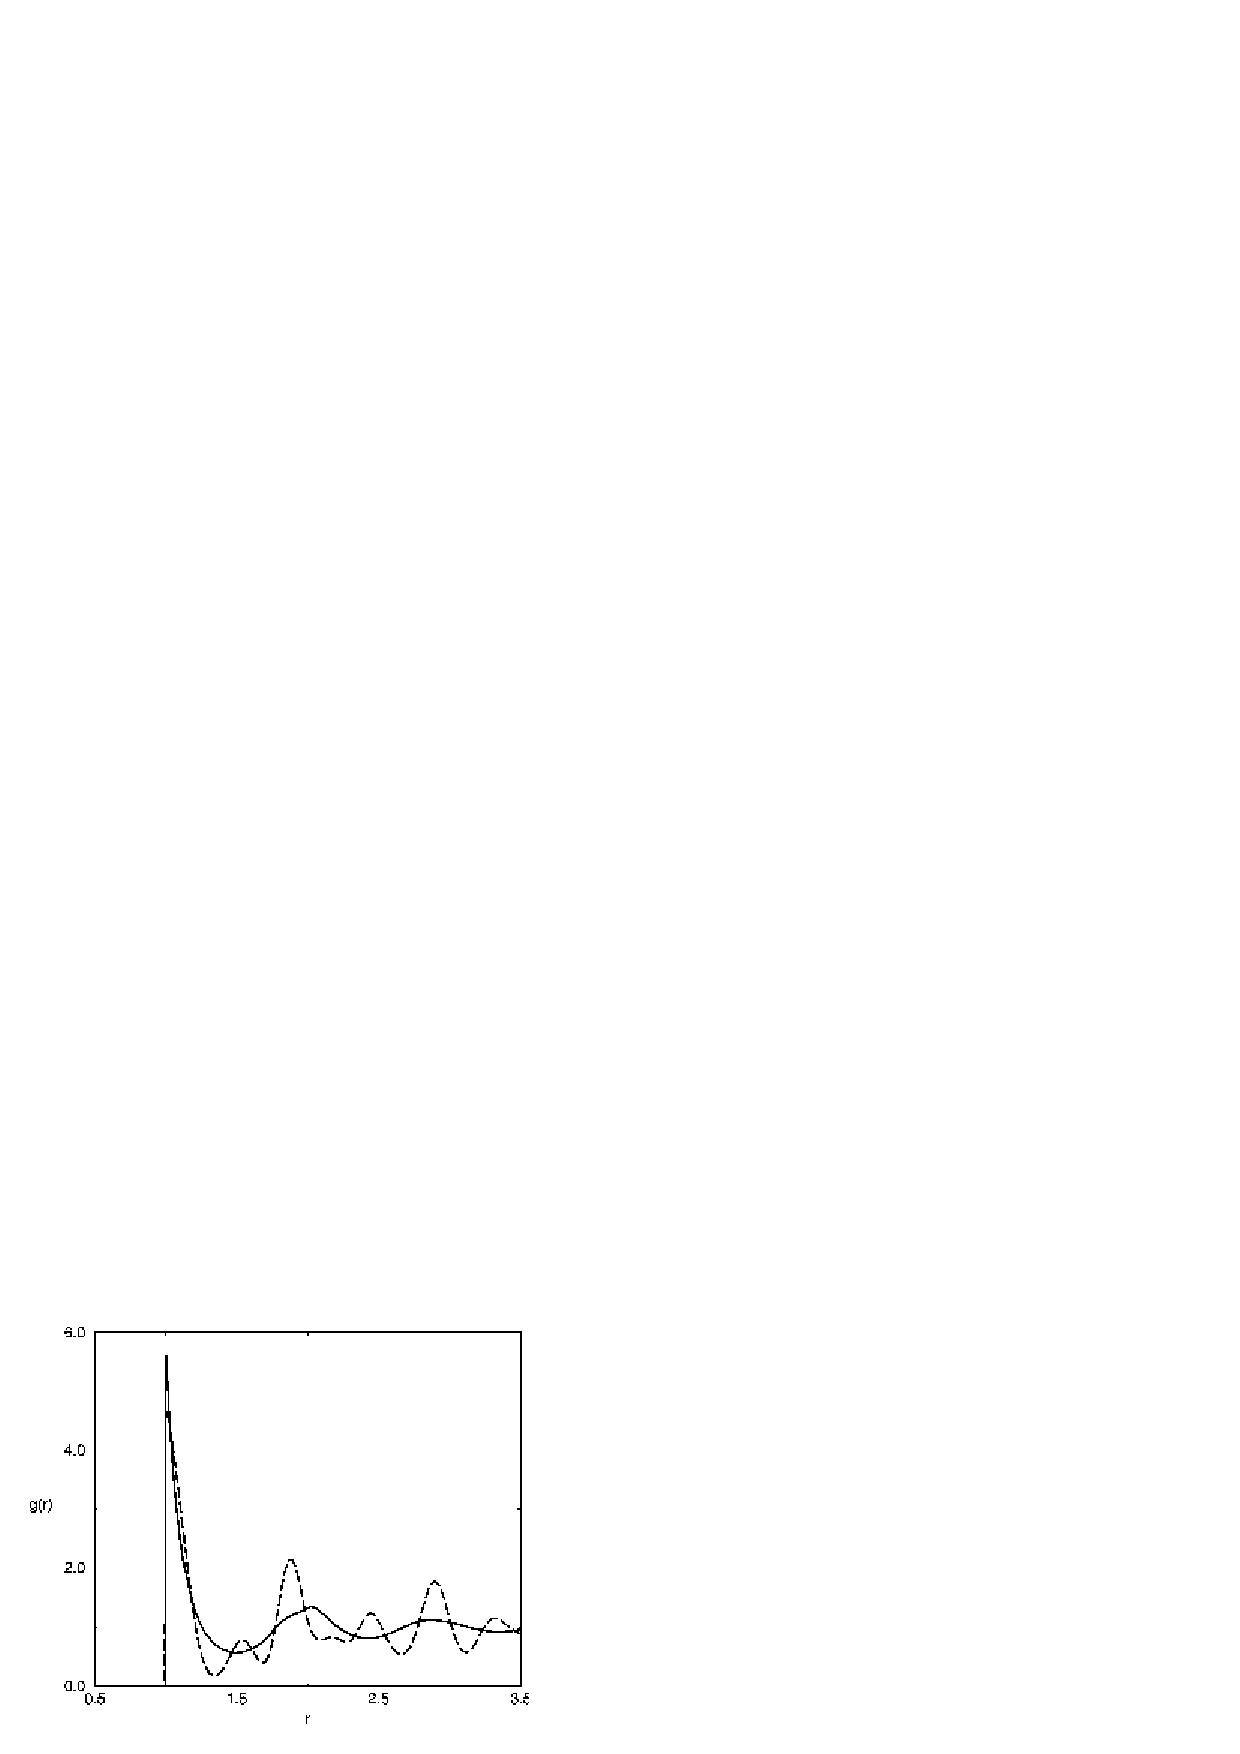
\includegraphics[width=0.4\textwidth]{rdf_XF}}
	\caption{Examples of \acf{RDF}.}
	\label{fig:rdf}
\end{figure}

The \acf{RDF} describes how the particle density varies as a function of the distance from one particular particle. It is defined as the ratio of the probability to find a particle at a distance $r$ of the central particle by the same quantity in the ideal gas:
\begin{equation}
	g(r) \equiv \frac{1}{N} \sum_{i}^N \frac{
		\sum_{j\neq i} \delta(r_{ij} - r)
		}{
		\int_V \rho \delta(r^\prime-r) dV
		}
	\label{eq:rdf}
\end{equation}
where $\rho$ is the number density. In the bulk, the numerator has a a simple expression independent of the central particle and $g(r)$ is written as:
\begin{equation}
	g(r) = \frac{
		\sum_{i}^N \sum_{j\neq i} \delta(r_{ij} - r)
		}{
		4\pi r^2 dr \rho(N-1)
		}
	\label{eq:rdf_bulk}
\end{equation}

By definition, in an ideal gas we have $g(r)=1$ for all distance $r$. For an dilute hard spheres gas, the \ac{RDF} is a step function: no particle within the hard core and uniform probability further. In a crystal, the \ac{RDF} presents thin peaks indicating a regular periodic arrangement. In a dense phase, the \ac{RDF} presents oscillations, or broad peaks that indicates preferred distances (see \FigureRef{fig:rdf}). The first peak is the first shell of particles around the reference particle; the second peak the second shell, etc.

When the \ac{RDF} presents a clear fist minimum as in \FigureRef{fig:rdf}, it is possible to use its position to define the maximum bond length $r_b$. Purely repulsive potentials (hard sphere, \ac{WCA}, etc.) satisfy this condition in dense phases.

In practice, the \ac{RDF} is an averaged function that does not contain information about local non-periodic structures. The \ac{RDF} is a real space function, but it is directly related to the static \ac{Sq} given by scattering experiments.
\begin{equation}
	S(q) = 1 + \rho \int {\exp{(-\imath \vec{q}\cdot\vec{r})} g(r)dr}
	\label{eq:rdf2Sq}
\end{equation}



\subsection{Voronoi diagram}

\begin{figure}
	\centering
	\subfloat[2D. Source Wikipedia]{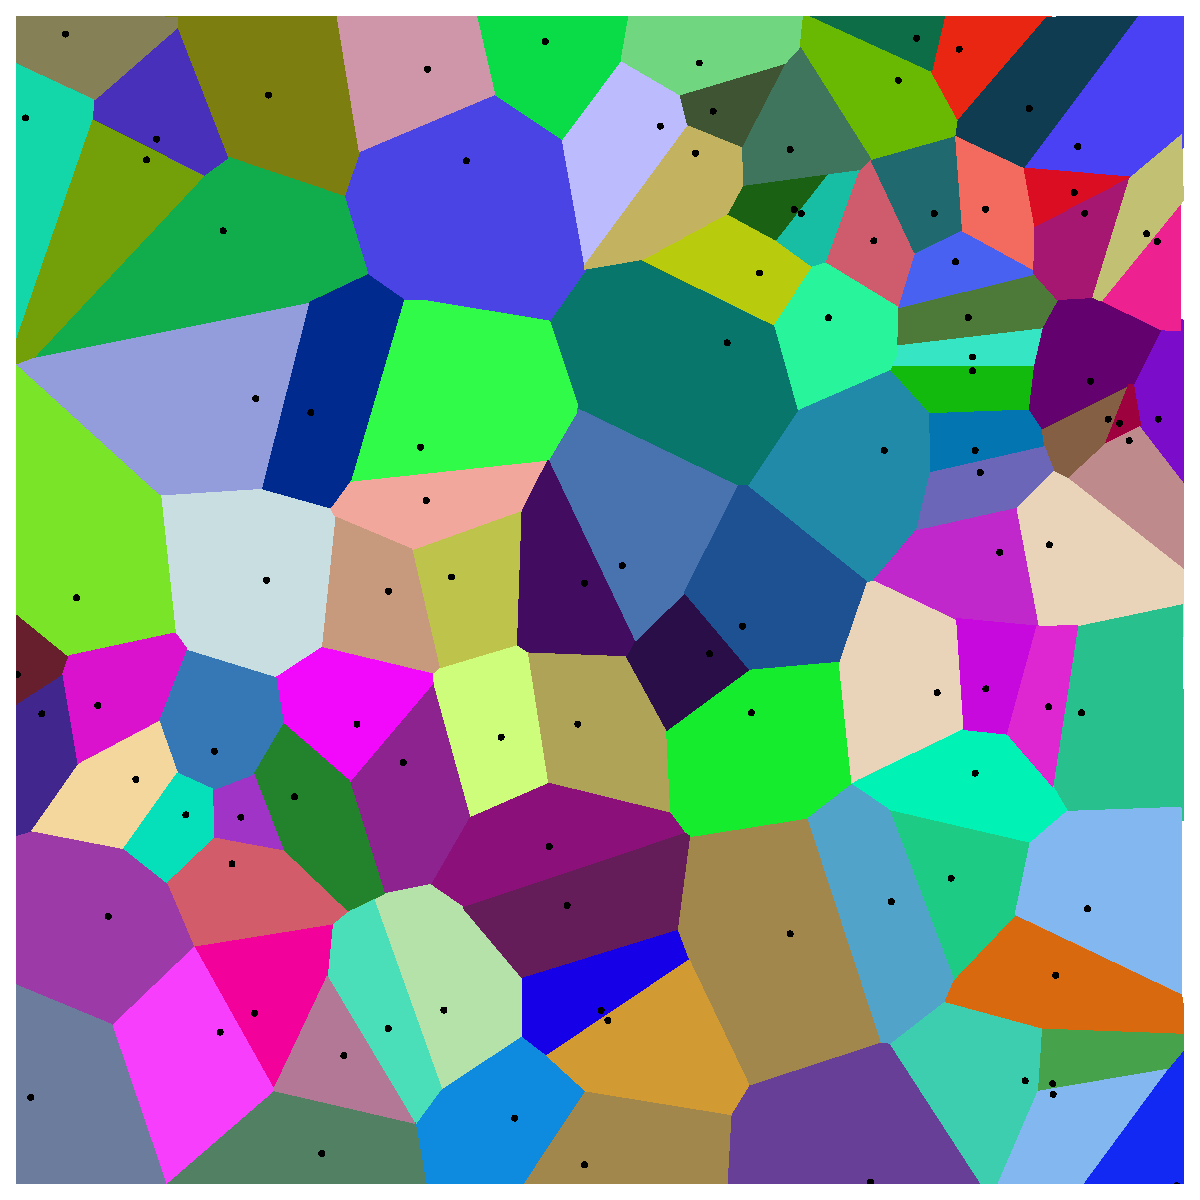
\includegraphics[width=0.45\textwidth]{voro2d}}
	\subfloat[3D. Source~\citep{rycroft2007multiscale}]{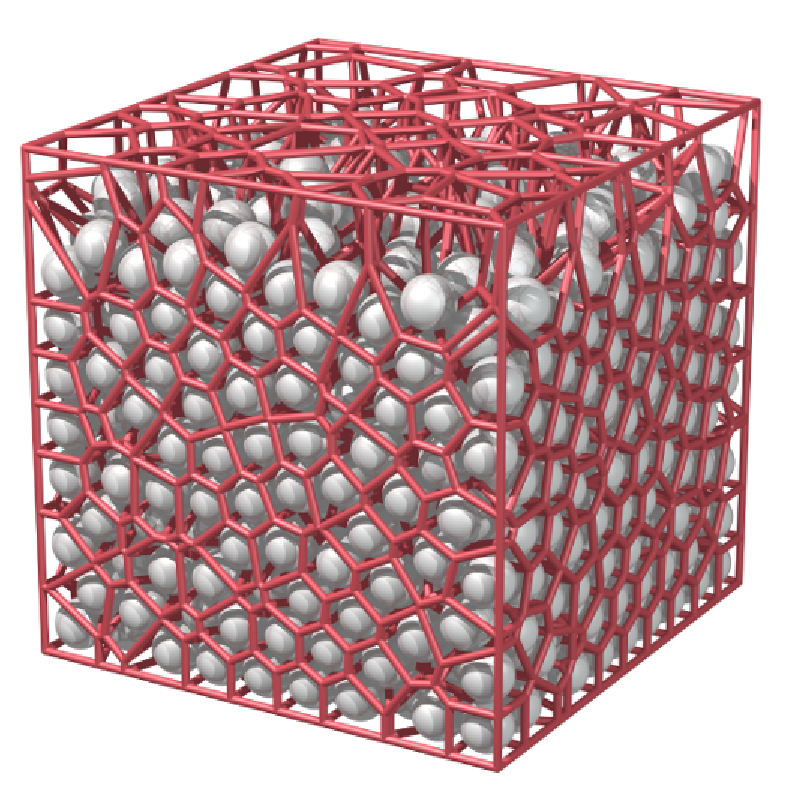
\includegraphics[width=0.45\textwidth]{voro3d_small}}
	\caption{Voronoi decomposition.}
	\label{fig:voro}
\end{figure}

Another method to select construct the bond graph is the Voronoi decomposition (see \FigureRef{fig:voro}). The space is split in cells, one per particle. The cell of the particle P contains all the points closer to P than to any other particle. In 2D the Voronoi cell is a convex polygon sharing a side with its neighbours. In 3D, the surface of a Voronoi cell is composed of flat polygons shared between two particles. A vertex is equidistant from more than two particles. If two particles share a surface and that the line that join them intersects this surface, we define the particles as bonded.

However, we have to keep in mind that the Voronoi decomposition can be very unstable. Around high order vertices (4 or more equidistant particles), even a very slight perturbation of the sites may change the diagram topology and therefore the bond graph~\citep{weller1997stability, ReintenWolde1996, Williams2007}. Some authors propose modified versions of the Voronoi decomposition with better stability. Each of these versions has a goal, for example selecting only the stable bonds~\citep{weller1997stability} or finding the high order vertices~\citep{Williams2007, rycroft2007multiscale} despite their instability.

Contrary to the maximum bond length method, the Voronoi decomposition potentially yields very anisotropic cells~\citep{Schroder-Turk2010}. Considering far-apart particles as bonded may obfuscate the meaning of local symmetries. Thus, in this thesis we prefer the maximum bond length method.

\subsection{Inherent structure}

We have seen in \SectionRef{sec:config_vib} that in dense phases, it is possible to decompose the entropy $S$ of the system between a configurational part $S_c$ and a vibrational part $S_v$. Conceptually, a particle vibrates around a (regular or not) lattice position. The structure we are interested in is this "lattice". Unfortunately, the thermal motion of the particles can alter both topology and geometry of the bond network, obscuring the underlying structure. 

Stilliger and co-workers~\citep{Stillinger1982, Stillinger1984} propose to quench numerically a given configuration, making each particle follow the steepest-descent path locally available on the energy landscape. After this process each particle sits at its local potential energy minimum. Performing the structural analysis on this "inherent structure" gives much sharper results (see \FigureRef{fig:inherent}).

Stilliger's method can be applied only to systems with a potential energy, not to athermal systems like hard spheres. For these systems, other methods were proposed, like fast inflation of the volume of the particle~\citep{Stillinger1985, berthier2009gtd} or averaging positions on short time~\citep{santen2000absence}.

One can argue that an experimental method giving the short-time average of the positions of the particles would yield in fact the inherent structure of the system. Because of the acquisition time, confocal microscope may already give such information.

\begin{figure}
	\centering
	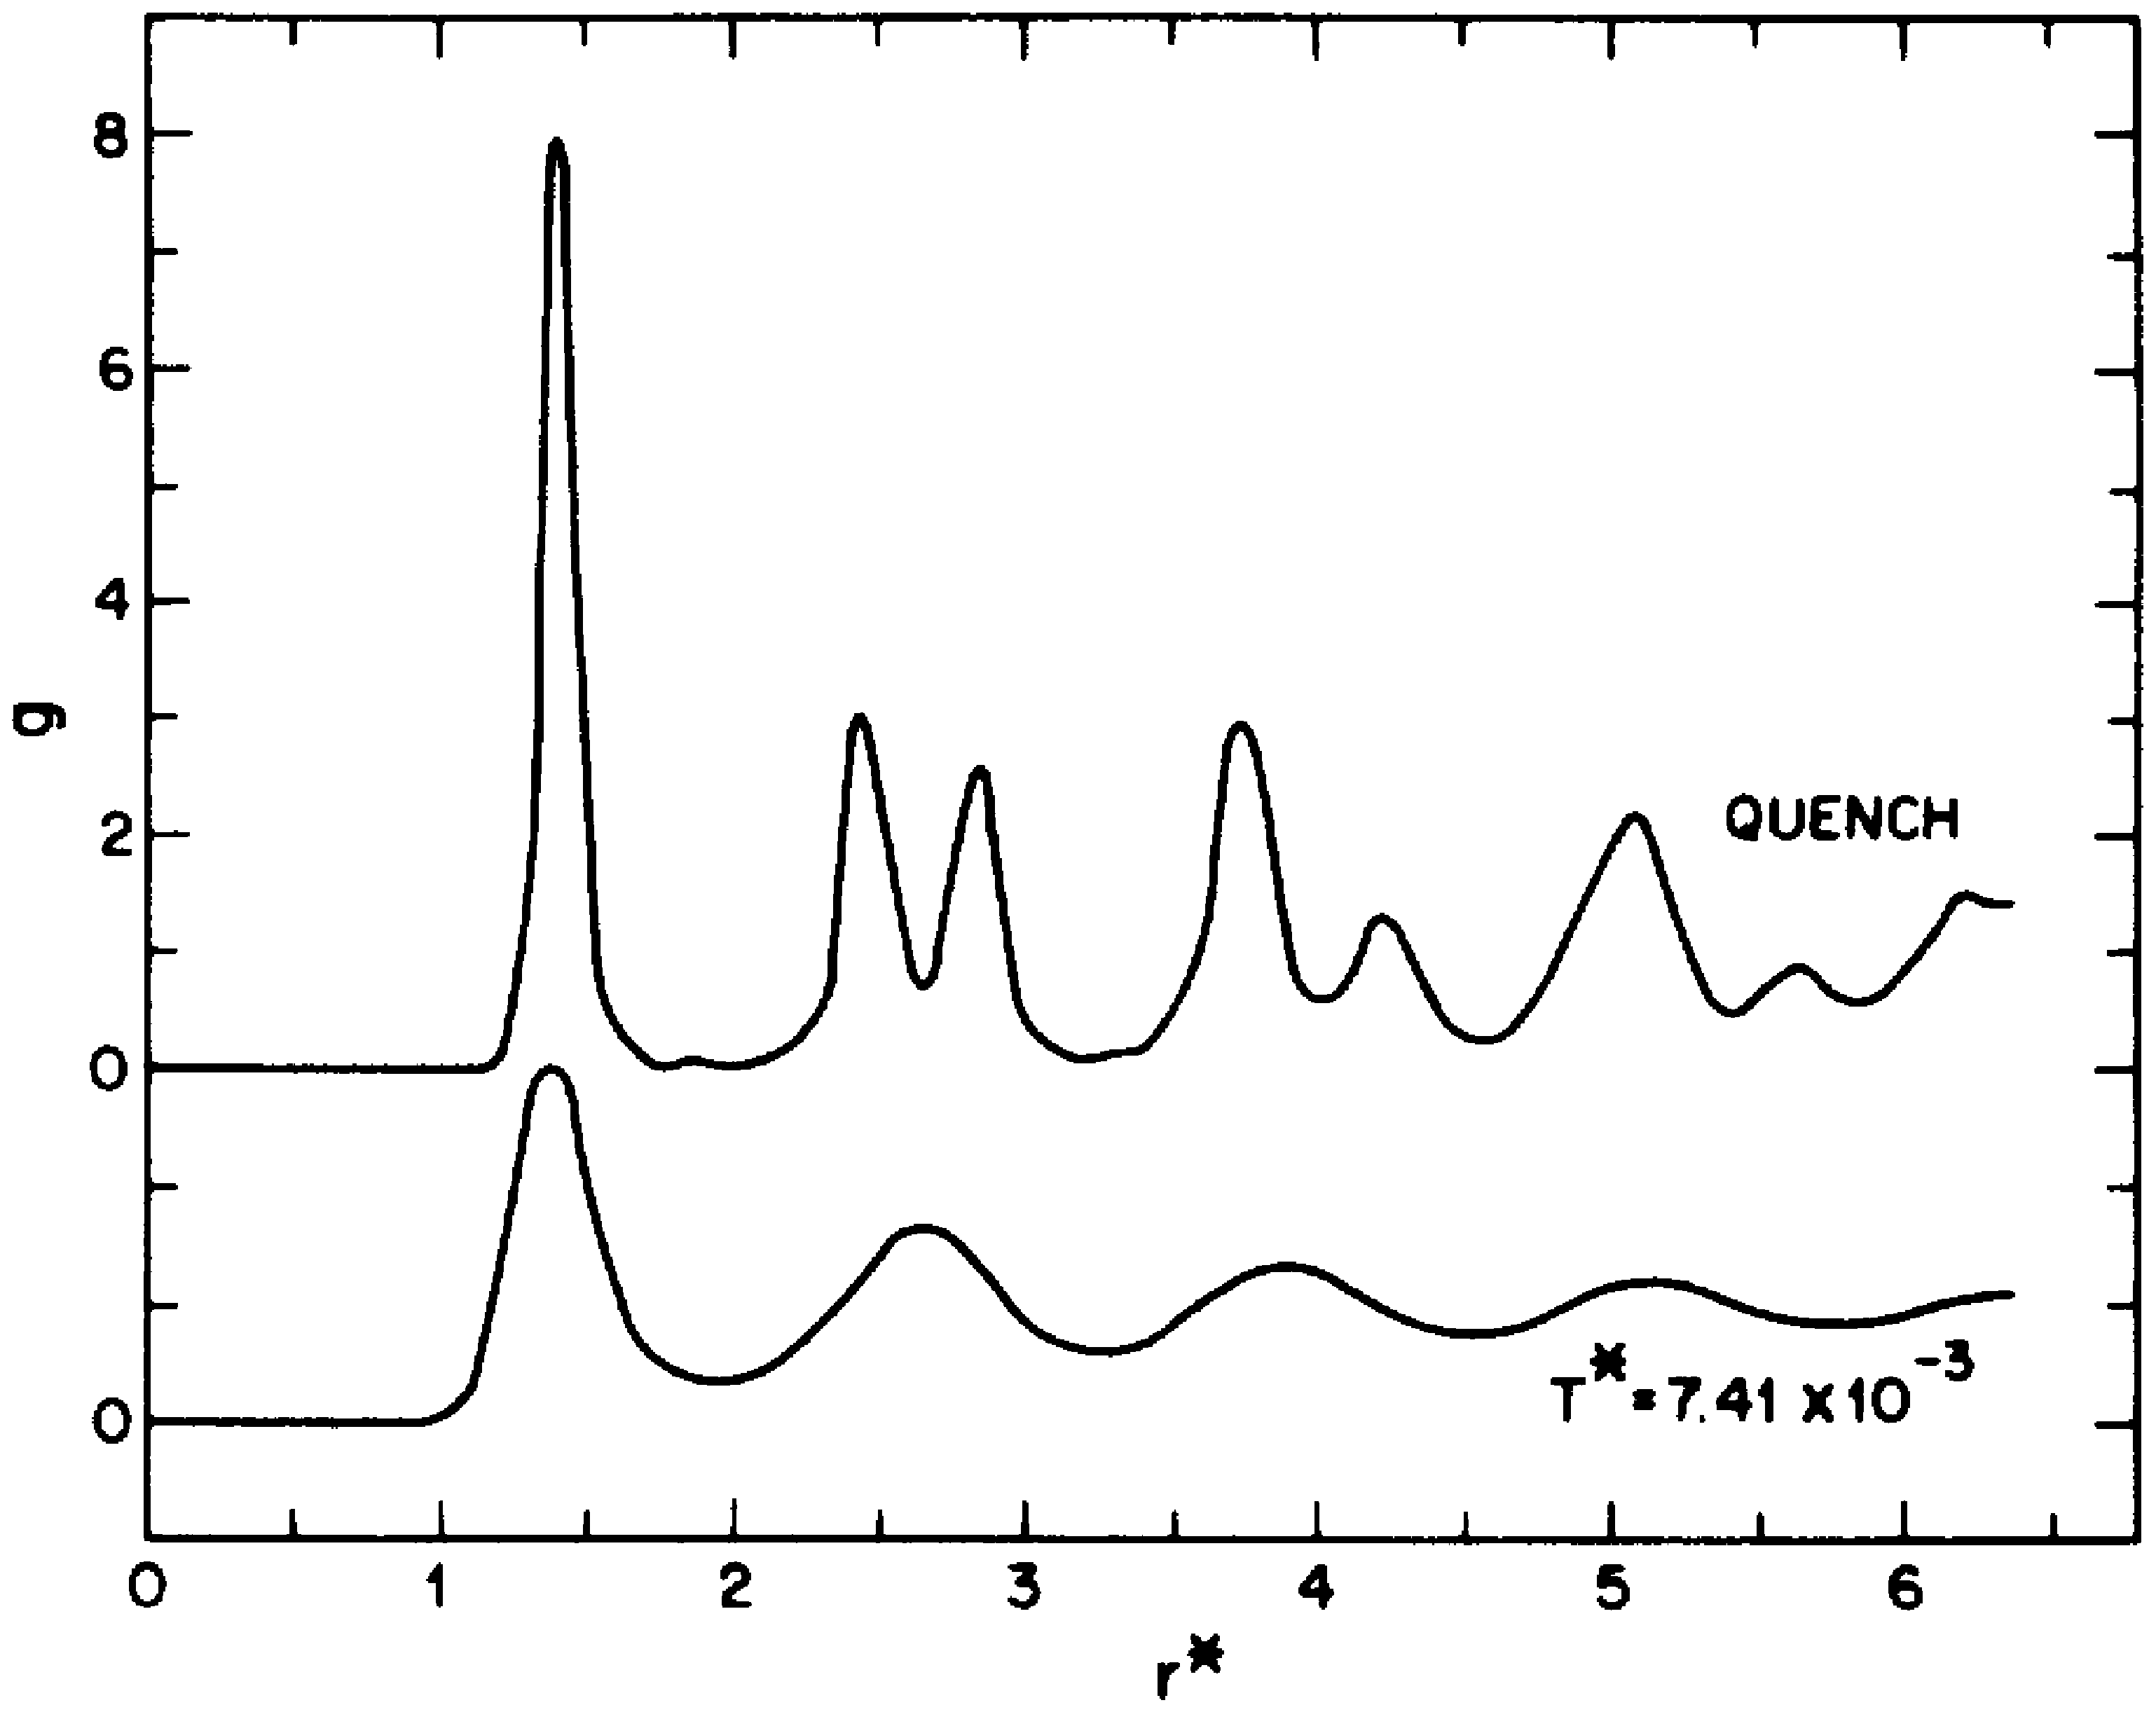
\includegraphics[width=0.6\textwidth]{steepest_descent}
	\caption{Radial distribution function of a fluid (Gaussian core model in 2D) and the corresponding "inherent structure". Source \ReferenceRef{Stillinger1982}.}
	\label{fig:inherent}
\end{figure}

\section{Topology of the bond network}

A first way to look for structure is to consider only the topology of the bond graph. Because topology is invariant by continuous deformations, topological methods give discrete variables, changing in a discontinuous manner in time and space.

\subsection{Coordination number}

Once the bond network established, it is straightforward to count the number of bonds per particle, also called coordination number. The coordination number is a very simple but rough way to categorise local structures. Actually, most of the particles in a system of monodisperse isotropic repulsing disks system will have 6 neighbours, even if they are not crystalline (see \FigureRef{fig:coordination}). The same is true in for repulsive spheres who have almost always 12 neighbours but various types of crystalline or non-crystalline orders.

\subsection{Voronoi cell shape}

\subsubsection{2D: Geometrical defects}

The importance of geometrical defects (voids) in 2D melting of a hexagonal crystal of monodisperse hard discs has been emphasised by Glaser and Clark~\citep{Glaser1990}. To emphasise the defects to the perfect triangular paving of the plan, they systematically decimate the bond graph obtained by Voronoi decomposition by removing the bonds longer than the maximum bond length. This reveals patches of triangles (crystal-like) and ladder-like clusters of squares or higher order polygons (defects) (see \FigureRef{fig:defects}).

\begin{figure}
	\centering
	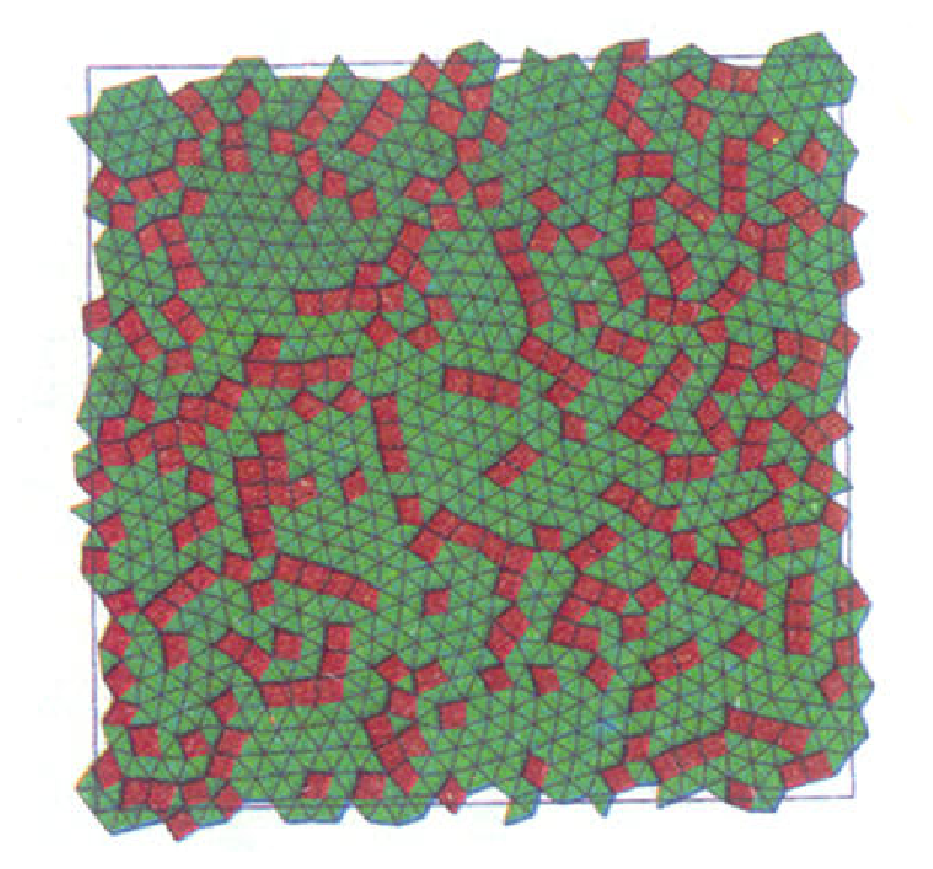
\includegraphics[width=0.6\textwidth]{defects}
	\caption{Bond network of a repulsive 2D liquid obtained by decimated Voronoi decomposition (see text). Triangles of bonds are shown in green, polygons of 4 or more bonds (defects) are shown in red. Source \ReferenceRef{Glaser1990}.}
	\label{fig:defects}
\end{figure}

\subsubsection{3D: Voronoi signature}

The shape of the Voronoi cell was often used in 3D to identify local structure~\citep{Duijneveldt1992, Cape1981, Hsu1979a, Nose1986, tanemura1977geometrical}. It is customary to define the signature of a Voronoi polyhedron as a set of integers $(n_3 ,n_4 ,n_5 ,\ldots)$, where $n_l$ is the number of $l$-sided faces of the polyhedron. For example, the Voronoi polyhedron of a perfect \ac{FCC} structure, the rhombic dodecahedron that has twelve lozenge-shaped faces, is denoted by $(0, 12, 0, 0, \ldots)$, while the Voronoi polyhedron of a particle in a \ac{BCC} structure, is denoted by $(0, 6, 0, 8, 0, \ldots)$ (six squares, eight hexagons).

In practice, the Voronoi signatures of the particles in a crystal will be modified by the thermal vibrations (see \FigureRef{fig:voroCell}). For instance, the characteristic Voronoi polyhedron of the \ac{FCC} lattice, the rhombic dodecahedron, will be removed by the tiniest thermal motion. Of the 14 vertices of the rhombic dodecahedron there are six where four faces meet. Any thermal motion will make these fourfold vertices break up into sets of threefold vertices connected by short edges. The result is that a variety of polyhedra such as $(0,3,6,4)$, $(0,3,6,5)$, $(0,4,4,6)$, $(0,4,4,7)$ occur in a thermally equilibrated \ac{FCC} crystal. Hence, Voronoi signatures can only be used in a statistical sense to identify solid-like particles.

\begin{figure}
	\centering
	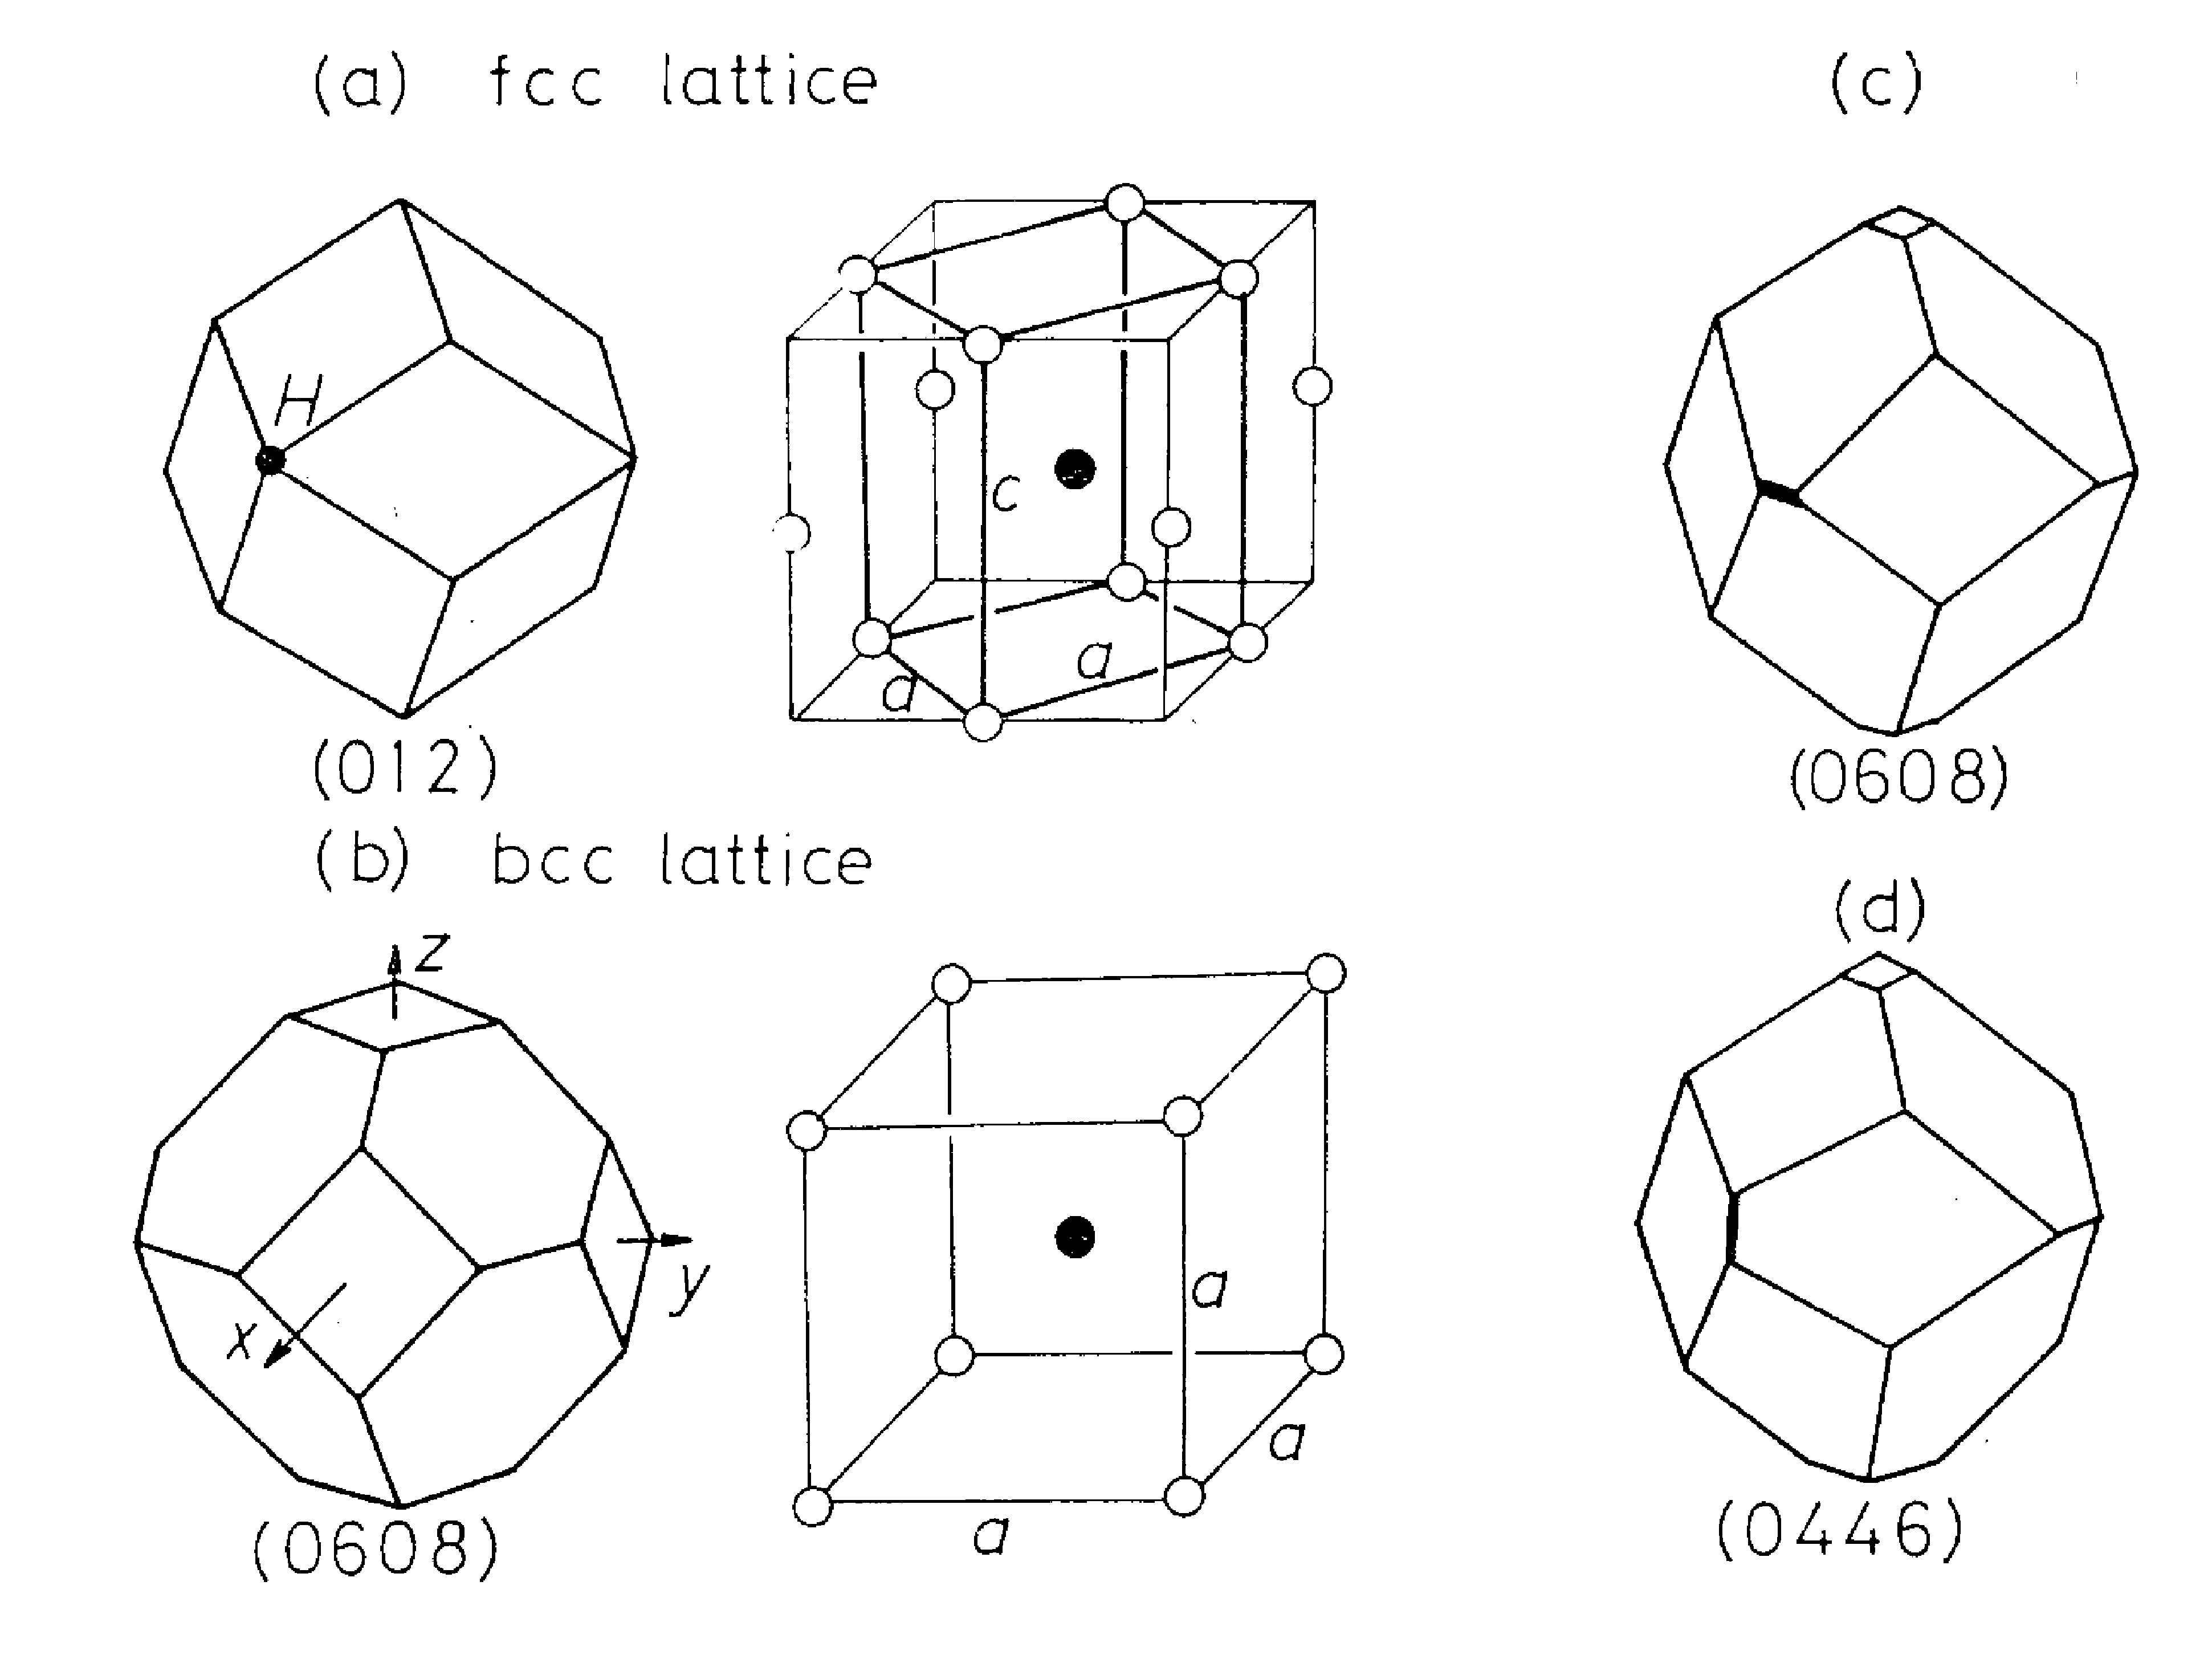
\includegraphics[width=0.6\textwidth]{voro_cell}
	\caption{Topological relations between $(0,6,0,8)$ and $(0,4,4,6)$ polyhedra. (a) \acs{FCC} lattice, (b) \acs{BCC} lattice. Black circles are centred atoms of respective Voronoi polyhedra. If the parallelepiped indicated by bold lines in (a) is compressed from top to bottom, it turns out to the unit cell of (b). (c) $(0,6,0,8)$ polyhedron, (d) $(0,4,4,6)$ polyhedron. If the horizontal bold line is replaced by the vertical, the $(0,6,0,8)$ polyhedron changes to the $(0,4,4,6)$ polyhedron and vice versa. Source \ReferenceRef{tanemura1977geometrical}}
	\label{fig:voroCell}
\end{figure}

\subsection{Common neighbours analysis}
\label{sec:commonNgb}

We know that any given particle has almost always 12 neighbours. Topological differences come when looking at the neighbours of the neighbours. Following this idea, \citet{Honeycutt1987} looked at the common neighbours of two particles A and B. They give 4 indices to characterise the pair:
\begin{enumerate}
	\item Are A and B bounded? (1 or 2)
	\item Number of neighbours common to A and B
	\item Number of bonds between the common neighbours
	\item Distinguishing between different arrangements of the bonds.
\end{enumerate}

They focus on two types of pairs: the 1551 and the 2331. The 1551 pair corresponds to two neighbouring particles with five common neighbours that form a pentagon of bonds. The 2331 pair corresponds to two particles that are not neighbours but have three common neighbours that form a triangle of bonds. The two types of pairs are characteristic of icosahedral ordering (see \FigureRef{fig:commonNgb}). 1421 and 1422 are characteristic of crystals.

\begin{figure}
	\centering
	\subfloat[1551-pair]{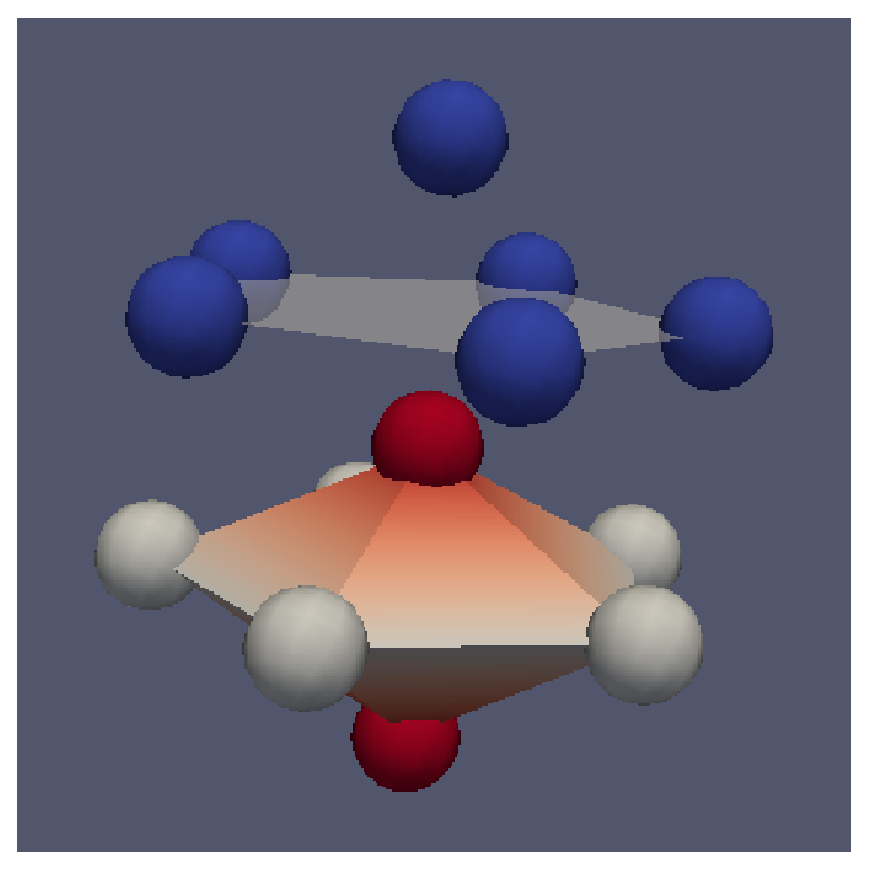
\includegraphics[width=0.3\textwidth]{ico_13_1551}}\quad
	\subfloat[2331-pair]{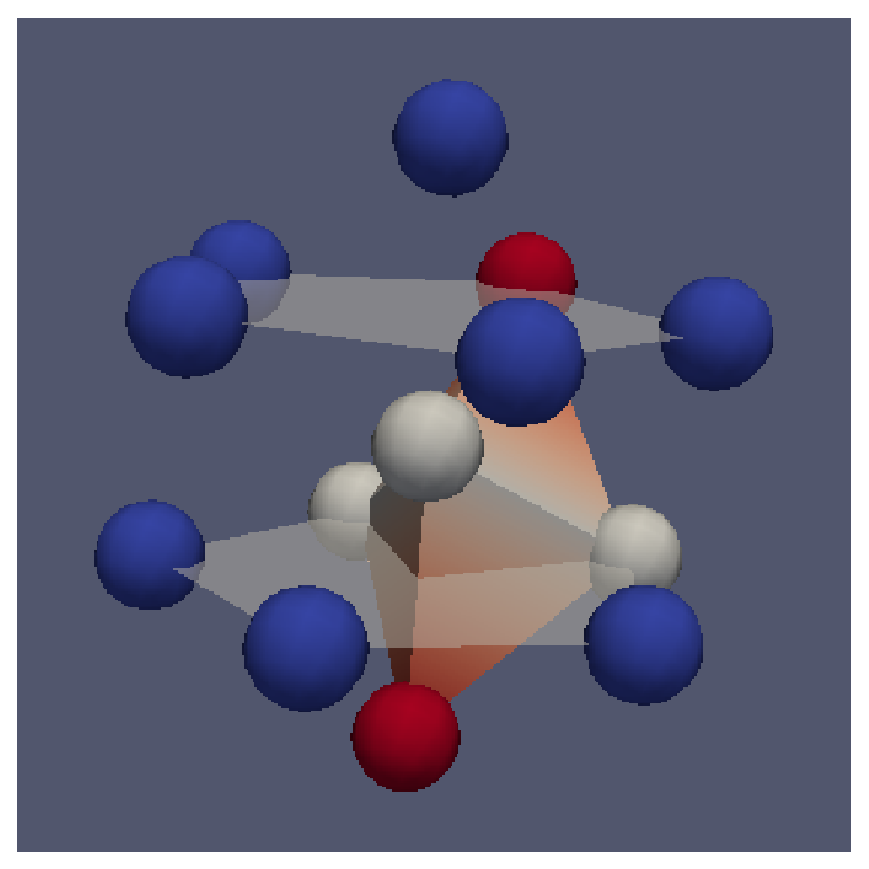
\includegraphics[width=0.3\textwidth]{ico_13_2331}}
	\caption{Characteristic pairs of 13-particles icosahedron. Red particles are the particles of the pair. White particles are the common neighbours. Blue particles are the rest of the icosahedron. Pairs are name in the common neighbour analysis terminology (see \SectionRef{sec:commonNgb}). Note that their are more than one pair of each type in the icosahedron.}
	\label{fig:commonNgb}
\end{figure}

\subsection{Topological cluster classification}
\label{sec:TCC}

The \acf{TCC} is a generalisation of the common neighbour analysis by Williams~\citep{Williams2007}. Its goal is to identify simple clusters inside a bulk phase. The selected clusters are the Morse clusters~\citep{doye1995effect} of less than 13 particles and the 13 atom clusters found in an \ac{FCC} and an \ac{HCP} crystal phase. One first search for 3, 4 and 5 membered shortest path (SP) rings~\citep{Franzblau1991}. A letter is then assigned to the ring depending on the number of particles bonded to all the ring's members: a for the ring alone; b if only one particle is bonded to all the ring's members; c for two particles, one on each side of the ring. In practice the SP5c and SP3c clusters corresponds to Jonsson and Andersen's 1551 and 2331 pairs respectively. The SPnx clusters are then combined to form larger clusters. A full icosahedral cluster contained 12 overlapping SP5c clusters is composed of two SP5c clusters sharing one spindle particle (see \FigureRef{fig:commonNgb}).

Analysing the results is a simple matter to record the atoms which form the various clusters. If some of the clusters have been identified multiple times this can be checked for and corrected later. However the reporting of population levels for the various clusters opens up choice and ambiguity. This is because any given atom may be a member of several different clusters. Williams reports the population levels in the following manner. If an atom is a member of a cluster and also a member of a different cluster which has more atoms it is only identified with the larger cluster. An atom may be a member of two clusters consisting of the same number of atoms, in this case the atom is reported as being a member of both clusters if it is not a member of any larger clusters. Using this approach we can construct a histogram of the net population levels for the various clusters (see \FigureRef{fig:tcc} for an example in hard sphere fluid).

\begin{figure}
	\centering
	\includegraphics[width=0.8\textwidth]{histTCC}
	\caption{A histogram of the net population levels for the various clusters in a hard sphere fluid. Source \ReferenceRef{Williams2007}.}
	\label{fig:tcc}
\end{figure}

\subsection{Limits of topological approaches}

Analysis of the topology of the bond network gives discrete categories of structures. Thus, one observes discrete jumps from one category to another both in time and in space. A common example is a cluster of particles that is detected alternatively in the categories A and B when followed in time. Is this cluster A or B? Do we need to create a new category A+B? How to describe the time correlation of these discrete structures? And how can we characterize the spatial extent of a collection of structures?

\section{Bond orientational order}
\label{sec:boo}

To go further into local structure analysis, one need to take into account both the topology of the bond network and its local symmetry.

\subsection{Hexatic order parameter - \texorpdfstring{$\psi_6$}{psi6}}

\begin{figure}
	\centering
	\includegraphics[width=0.8\textwidth]{coordination}
	\caption{Relationship between dynamic heterogeneity, medium-range crystalline order, and topological defects for a quasi-2D driven granular matter system. (a) Particle trajectory during $t_0 < t < t_0 +\tau_\alpha$ ($t_0$: arbitrary). (b) Spatial distribution of the time-averaged ($t_0 < t < t_0 +\tau_\alpha$) bond-orientational order parameter $\psi_6$. (c) Spatial distribution of the coordination number Z at $t = t_0$. Clusters of particles with high crystalline order in (b) and the corresponding region in (a) and (c) are circled for a guide to the eye. Note that almost all the particles have a coordination number $Z=6$ but display a wide range of $\psi_6$. Source \ReferenceRef{watanabe2008}}
	\label{fig:coordination}
\end{figure}

In 2D, it is possible to define the hexatic order parameter~\citep{Nelson1979, Binder2002, Hamanaka2006, kawasaki2007cbd} $\psi_6$ to detect the degree of six-fold symmetry around given particle $i$:
\begin{equation} 
	\psi_{6}^{i}=\frac{1}{n_i}\sum^{n_i}_{k=1}e^{j6\theta^i_{k}} 
\end{equation}
where $n_i$ is the number of nearest neighbours of particle $i$, and $\theta^i_k$ is the angle between $\vec{r}_{ik} = \vec{r}_k - \vec{r}_i$ and the x axis, where particle $k$ is a neighbour of particle $i$ ($j$ is the imaginary number). $\psi_{6}^{i}=1$ means the perfect hexagonal arrangement of six nearest-neighbour particles around particle $i$ and $\psi_{6}^{i}=0$ means a random arrangement.

One can follow the averaged order parameter $\psi_6= \langle \psi^{i}_{6} \rangle$ to study the liquid to hexatic to crystal phase transition, or the link between local order and dynamics (see \FigureRef{fig:coordination}). Moreover, $\psi_{6}^{i}$ is a continuous, local order parameter, defined at the particle level. It is then possible to define its spatial correlation $g_6(r) = |\langle \psi_6^k \psi_{6}^{l} \rangle|$, with $r = |\vec{r_l} - \vec{r_k} |$. $g_6(r)$ should decay to zero if the hexatic order is only local.

Steinhardt's bond orientational order (BOO)~\citep{steinhardt1983boo} is the generalised analog in 3D of the hexatic bond orientational order. To understand its meaning we need to explain some mathematics.

\subsection{Spherical harmonics}

\begin{figure}
	\centering
	\subfloat[$\ell=4$, $m=0$]{\label{fig:sh4-0}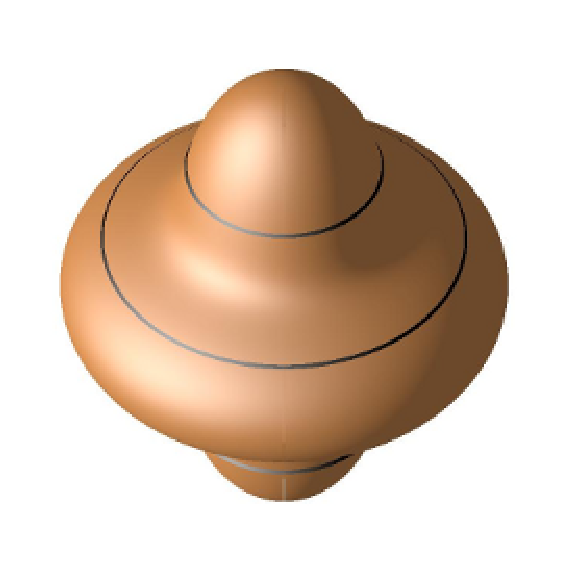
\includegraphics[width=0.25\textwidth]{sh4-0}}
	\subfloat[$\ell=4$, $m=4$]{\label{fig:sh4-4}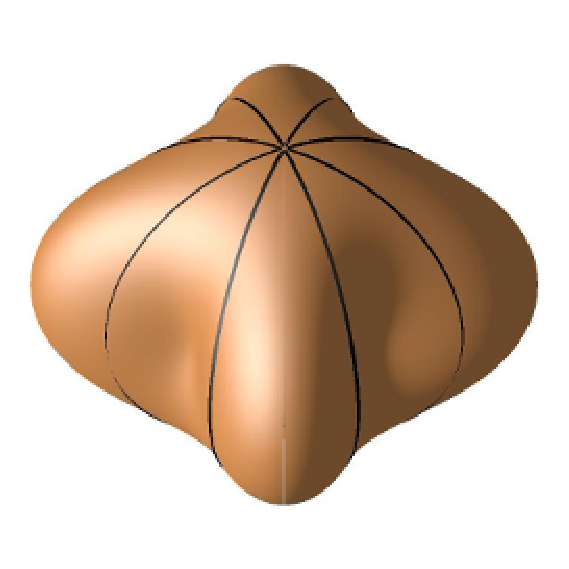
\includegraphics[width=0.25\textwidth]{sh4-4}}
	\subfloat[$\ell=10$, $m=10$]{\label{fig:sh10-10}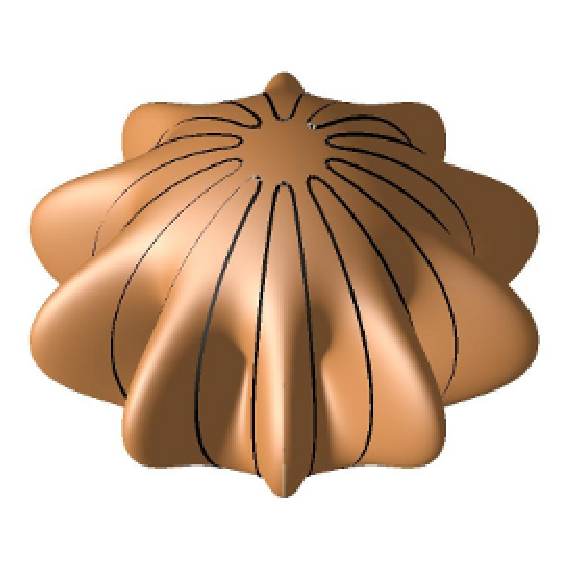
\includegraphics[width=0.25\textwidth]{sh10-10}}\\
	\subfloat[$\ell=6$, $m=0$]{\label{fig:sh6-0}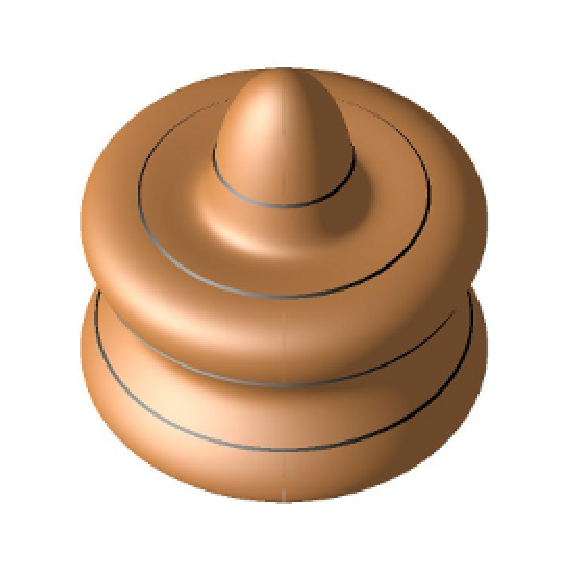
\includegraphics[width=0.25\textwidth]{sh6-0}}
	\subfloat[$\ell=6$, $m=3$]{\label{fig:sh6-3}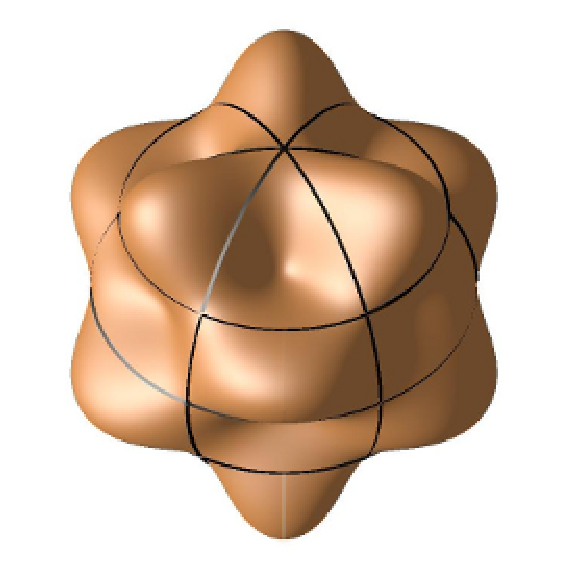
\includegraphics[width=0.25\textwidth]{sh6-3}}
	\subfloat[$\ell=6$, $m=5$]{\label{fig:sh6-5}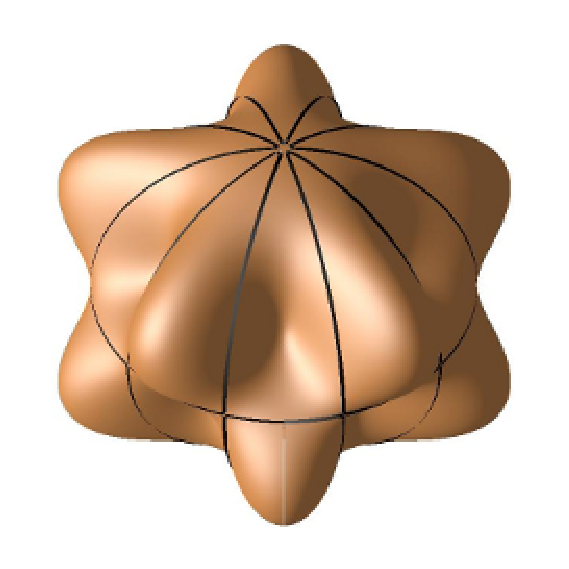
\includegraphics[width=0.25\textwidth]{sh6-5}}
	\subfloat[$\ell=6$, $m=6$]{\label{fig:sh6-6}\includegraphics[width=0.25\textwidth]{sh6-6}}
	\caption{Spherical Harmonics at various order and degree. Note how a \acs{FCC} cluster can be approximated by the sum of \subref{fig:sh6-6} for the hexatic plane and \subref{fig:sh6-3} for the upper and lower planes. In the same way the two 5-particle rings of an Icosahedron look like \subref{fig:sh6-5} whereas the spindle atoms can be described by \subref{fig:sh6-0}. \subref{fig:sh10-10} is common to both Icosahedron and Dodecahedron. Source \ReferenceRef{AllenMcNamara}.}
	\label{fig:SphericalHarmonics}
\end{figure}

\begin{figure}
	\centering
	\def\svgwidth{0.6\textwidth}\input{earth_spectrum.pdf_tex}
	\caption{Spectrum of the earth topography. y axis is in meters. The curve is decreasing, meaning that the lower degrees (long wavelength) are of larger amplitude than the higher degrees (short wavelength). Source \ReferenceRef{Vigny}.}
	\label{fig:earth_spectrum}
\end{figure}

The spherical harmonics $Y_{\ell m}(\theta,\phi)$ are an infinite orthogonal base of functions. All fields (solution of Laplace equation) on a sphere can be decomposed into spherical harmonics. $\ell \geq 0$ indicates the order of symmetry. $m$, with $-\ell \geq m \geq \ell$, indicates the orientation with respect to a referent set of orthonormal axes. \FigureRef{fig:SphericalHarmonics} represents a few spherical harmonics.

Let us give a concrete example: earth topology. In first approximation, planet earth is a sphere, but this sphere has some roughness (Mount Fuji is a roughness of 3,776 m compared to sea level). We note $h(\theta,\phi)$ the altitude of the surface of the earth compared to sea level at latitude $\theta$ and longitude $\phi$. This field can be decomposed into an infinite sum of spherical harmonics:
\begin{equation} 
h(\theta,\phi) = \sum_{\ell=0}^{\infty} \sum_{m=-\ell}^{\ell} q_{\ell m} Y_{\ell m}(\theta,\phi)
\end{equation}
The $q_{\ell m}$ coefficients are complex numbers. The spectrum of the field $h(\theta,\phi)$ is the sequence of number $SP_\ell$ giving the amplitude of the term $\ell$ in the spherical harmonics decomposition (see \FigureRef{fig:earth_spectrum}).
\begin{equation} 
	SP_\ell = \sqrt{\frac{1}{4\pi} \sum_{m=-\ell}^{\ell} |q_{\ell m}|^2 } 
\end{equation}

Terms with small $SP_\ell$ can be neglected to give an approximation of the field $h(\theta,\phi)$. The more terms that are left, the better the approximation(see \FigureRef{fig:earthApprox})

\begin{figure}
	\centering
	%\subfloat[$\ell=0$]{\includegraphics[width=0.3\textwidth]{earth_l0}}
	\subfloat[$\ell=1$]{\includegraphics[width=0.3\textwidth]{earth_l1}} 
	\subfloat[$\ell=2$]{\includegraphics[width=0.3\textwidth]{earth_l2}} 
	\subfloat[$\ell=3$]{\includegraphics[width=0.3\textwidth]{earth_l3}}\\
	\subfloat[$\ell=4$]{\includegraphics[width=0.3\textwidth]{earth_l4}} 
	\subfloat[$\ell=5$]{\includegraphics[width=0.3\textwidth]{earth_l5}} 
	\subfloat[$\ell=6$]{\includegraphics[width=0.3\textwidth]{earth_l6}}
	\caption{Spherical harmonics decomposition of earth topography. Source \ReferenceRef{Vigny}.}
	\label{fig:earth_decompo}
\end{figure}
\begin{figure}
	\ContinuedFloat
	\centering
	\subfloat[$\sum_{\ell=0}^6$]{\includegraphics[width=0.45\textwidth]{earth_to6}} 
	\subfloat[$\sum_{\ell=0}^{16}$]{\includegraphics[width=0.45\textwidth]{earth_to16}}\\
	\subfloat[$\sum_{\ell=0}^{36}$]{\includegraphics[width=0.45\textwidth]{earth_to36}} 
	\subfloat[Full grid of earth topography (6 data points per degree)]{\includegraphics[width=0.45\textwidth]{earth_grid}}
	\caption{Approximations of earth topography by partial sums of spherical harmonics. Source \ReferenceRef{Vigny}.}
	\label{fig:earthApprox}
\end{figure}

\subsection{Characterisation of the bonds}

Each bond $\vec r$ can be associated with the set of spherical harmonics $Y_{\ell m}(\theta(\vec r),\phi(\vec r))$. For even $\ell$, there is no need to give a directionality to the bond. Often, the analysis is performed only on the $\ell=4$ and $\ell=6$ orders, the two first non-zero even orders in the spectrum (averaged over all bonds in the system). Some authors go up to $\ell=8$ and $\ell=10$~\citep{Chakravarty2002}.

The whole system is characterised by the coefficients $\bar{q}_{\ell m} = \langle Y_{\ell m}(\vec r) \rangle$ where the average is taken over all the bonds. Each particle $i$ is characterised by the coefficients
\begin{equation}
	q_{\ell m}(i) = \frac{1}{N_i}\sum_{0}^{N_i} Y_{\ell m}(\theta(\vec r_{ij}),\phi(\vec r_{ij}))
	\label{eq:qlm}
\end{equation}
where the $\vec{r}_{ij}$ are all the bonds starting from $i$. We call the $q_{\ell m}$ defined by \EquationRef{eq:qlm} the local tensorial bond orientational order parameter.

Other sums are possible, like adding the surface bonds into \EquationRef{eq:qlm}, \latin{i.e.} the bond $r_{jk}$ with $j$ and $k$ neighbours of $i$. The tensorial order parameter $q_{\ell m}$ can be calculated in this way for any subset of bonds. For example, any cluster found by a topological method can be considered as a set of bonds and thus have an associated $q_{\ell m}$.

\subsection{Invariants}
\label{sec:boo_invariants}
Because $q_{\ell m}$ can be scrambled drastically by a rotation of the coordinate system, it is important to consider combinations invariant by rotation like a normalised version of the spectrum coefficients:
\begin{align}
	q_\ell =& \sqrt{\frac{4\pi}{2l+1} \sum_{m=-\ell}^{\ell} |q_{\ell m}|^2 }\label{eq:ql}\\
	w_\ell =& \frac{
		\sum\limits_{m_1+m_2+m_3=0} 
			\left( \begin{array}{ccc}
				\ell & \ell & \ell \\
				m_1 & m_2 & m_3 
			\end{array} \right)
			q_{\ell m_1} q_{\ell m_2} q_{\ell m_3}
	}{
		\left(
			\sum\limits_{m=-\ell}^{\ell} |q_{\ell m}|^2
		\right)^{\frac{3}{2}}
	} \label{eq:wl}
\end{align}

The term in brackets is the Wigner 3-j symbol~\citep{Landau1965}. $q_\ell$ is always positive and indicates the strength of the $\ell$ fold symmetry. For instance, $q_6$ has high values for \ac{BCC}, \ac{HCP} and \ac{FCC} crystals as for icosahedron. $w_\ell$ can be positive or negative and gives more precise information about the symmetry group. For instance, Steinhardt \latin{et al.} showed that $w_6$ reaches its absolute minimum value only in the case of perfect icosahedral order:
\begin{equation}
w_6^{ico}= -\frac{11}{\sqrt{4199}} \sim -0.169
\label{eq:w6ico}
\end{equation}

Generally, the sign of $w_\ell$ indicates the parity of the $\ell$ fold symmetry. For example (see \FigureRef{fig:basicClusters}), \ac{HCP} and \ac{FCC} crystals have both high $q_6$ because they have both hexatic planes. But a \ac{HCP} crystal is made of the repetition of only two hexatic planes ($ABAB\ldots$), so its symmetry is even. Whereas a \ac{FCC} crystal is made of three planes ($ABCABC\ldots$) so its symmetry is odd. \ac{HCP}'s $w_4$ is positive and \ac{FCC}'s $w_4$ is negative. See \TableRef{tab:rotational_invarients} for the values of the rotational invariants for some basic structures.

\begin{table}
	\begin{center}
	\begin{tabular}{|l|r|r|r|r|r|r|r|r|}
		\hline
		Structure & $q_4$ & $q_6$ & $q_8$ & $q_{10}$ & $w_4$ & $w_6$ & $w_8$ & $w_{10}$ \\ \hline
		Ico. & 0 & 0.6633 & 0 & 0.3629 & $\infty$ & -0.1697 & $\infty$ & -0.0939 \\ \hline
		\ac{HCP} & 0.0972 & 0.4848 & 0.3170 & 0.0102 & 0.1341 & -0.0124 & 0.0513 & -0.0799 \\ \hline
		\ac{FCC} & 0.1909 & 0.5745 & 0.4039 & 0.0129 & -0.1593 & -0.0132 & 0.0584 & -0.0901 \\ \hline
		\ac{BCC} 9 & 0.5092 & 0.6285 & 0.2128 & 0.6502 & -0.1593 & 0.0132 & 0.0585 & -0.0901 \\ \hline
		\ac{BCC} 15 & 0.0364 & 0.5107 & 0.4293 & 0.1952 & 0.1593 & 0.0132 & 0.0585 & -0.0901 \\ \hline
		Dodec. & 0.0530 & 0.4298 & 0.1386 & 0.1401 & -0.1341 & -0.0937 & 0.0918 & 0.0077 \\ \hline
	\end{tabular}
	\end{center}
	\caption{Rotational invarients of a few perfect structures. $q_{\ell}$ are obtained from \EquationRef{eq:qlm} and \EquationRef{eq:ql}.}
	\label{tab:rotational_invarients}
\end{table}

In theory, every possible local structure could be identified using local bond orientational invariants. In practice, local bond order parameters are used in diverse ways. For instance, in \ReferenceRef{Desgranges2008}, the crystalline structure around a given particle is characterised by its position in the two dimensional $(q_4, q_6)$-plane and $(q_4, w_4)$-plane. Using this approach, one can determine the type of structure occurring around each individual particle. The values of the local invariants are in fact broadly distributed because of thermal fluctuations (see top of \FigureRef{fig:invariants_maps}). It is often not possible to tell if one given particle is in one structure or another.

Frenkel and co-workers~\citep{Moroni2005, wolde:9932, wolde1999homogeneous, Volkov2002} analysed the structure of crystalline clusters in terms of order parameter distributions. To do that, they first computed the distributions of $q_4$ and $q_6$ for the liquid and for perfect \ac{FCC} and \ac{BCC} crystals. Due to thermal fluctuations, these distributions can be rather broad (see \FigureRef{fig:invariantsFit}). Then, they determined the distributions of the same order parameters in the crystalline cluster. These distributions are represented as a superposition of the distribution functions of the perfect phases. The superposition coefficients $c_{FCC}$, $c_{BCC}$ and $c_{LIQ}$, determined by mean square minimisation, then yield information on the composition of the cluster. For instance, $c_{FCC} \approx 0.5$, $c_{BCC} \approx 0.5$, and $c_{LIQ} \approx 0$ would be indicative of a cluster that is half in the \ac{FCC} structure and half in the \ac{BCC} structure.

\begin{figure}
	\centering
	\includegraphics[width=0.8\textwidth]{gasser_invariants}
	\caption{(A) $q_4$, $q_6$, and $w_6$ bond-order parameter histograms for \acs{FCC} (blue curves), \acs{HCP} (red curves), \acs{BCC} (black curves), and liquid (purple curves). (B) The measured bond-order histograms (black plots) of a colloidal hard sphere sample with $\phi=0.45$ are shown together with a least squares fit (blue curve) using the bond-order histograms from (A). Source \ReferenceRef{Gasser2001}.}
	\label{fig:invariantsFit}
\end{figure}

\subsection{Correlations}
\label{sec:boo_correl}

Besides the rotational invariants, we can quantify the correlation between the $\ell$-fold symmetry around particle $i$ and particle $j$ by the following dot product:
\begin{equation}
	s_\ell(i,j) = \frac{
		\sum_{m=-\ell}^{\ell} q_{\ell m}(i) q_{\ell m}^{*}(j)
	}{
		\sqrt{\sum_{m=-\ell}^{\ell} |q_{\ell m}(i)|^2} \sqrt{\sum_{m=-\ell}^{\ell} |q_{\ell m}(j)|^2}
	}
	\label{eq:boo_dot_product}
\end{equation}

By definition $s_\ell(i,i)=1$. Note that this correlation depends on the relative orientation of the two environments: two exactly similar environments rotated one compared to the other by angles inconsistent with the $\ell$-fold symmetry would give low or even negative values of $s_\ell(i,j)$. Furthermore, $s_6(i,j)$ does not differentiate between two well oriented icosahedron and two well oriented \ac{FCC} neighbourhoods: both pairs would be strongly correlated.

The radial correlation function of the tensorial bond order can then be defined as:
\begin{equation}
	g_\ell(r) \equiv \frac{1}{N}\sum_i^N \frac{
		\sum_{j \neq i}{ s_\ell(i,j) \delta\left(\left\|\vec{r}_i-\vec{r}_j \right\| - r \right)}
	}{
	\sum_{j \neq i}{\delta\left(\left\|\vec{r}_i-\vec{r}_j \right\| - r \right)}
	}
	\label{eq:boo_space_correl}
\end{equation}

Tensorial correlations can also be defined in time in the spirit of \EquationRef{eq:boo_dot_product} by taking $i$ and $j$ at different times. Note that this tensorial time correlation is not robust to the global rotation of a cluster keeping the same structure.
\begin{equation}
	g_\ell(t) \equiv \left\langle \frac{
		\sum_{m=-\ell}^{\ell} q_{\ell m}(i, t_0) q_{\ell m}^{*}(i, t_0+t)
	}{
		\sqrt{\sum_{m=-\ell}^{\ell} \left\|q_{\ell m}(i,t_0)\right\|^2}
	}\right\rangle_{i, t_0}
	\label{eq:boo_time_correl}
\end{equation}


\subsection{Cluster detection}
\label{sec:X_bonds}

In order to study nucleation growth of crystals, one need to be able to know for sure if a particle is within a crystalline cluster or not. As we saw before, the local invariants $q_{\ell}(i)$ have broad distributions. Many insulated high $q_6$ particles are detected in a fluid. Frenkel \latin{et al.}~\citep{wolde:9932} had the idea to look at $s_6(i,j)$ when $i$ and $j$ are neighbouring particles. The bond $r_{ij}$ is considered a crystalline bond if $s_{ii}>0.5$. A particle is crystalline-like if its number of crystalline bonds is above a certain threshold, typically between 6 and 8. If a particle has less crystalline bonds, it is considered to be liquid-like. Using this criterion to distinguish crystalline-like from liquid-like particles one can then search for clusters of connected solid-like particles.

\begin{figure}
	\centering
	\includegraphics[width=0.8\textwidth]{gasser_nucleus}
	\caption{Four snapshots during crystallisation of a sample with $\phi=0.45$. The red spheres are drawn to scale and represent particles that were identified as crystal-like. The particles in the metastable liquid state are shown by the blue spheres, reduced in size for clarity. (A) Time $t=\unit{20}{\minute}$ after shear melting, (B) $t=\unit{43}{\minute}$, (C) $t=\unit{66}{\minute}$, and (D) $t=\unit{89}{\minute}$. Source \ReferenceRef{Gasser2001}}
	\label{fig:nucleus}
\end{figure}

This procedure very efficiently distinguishes between periodic environments and non-periodic environments, but does not discriminate between different crystal structures. Furthermore, it is not picking up the aperiodic structures like icosahedra. As noted by \citet{Tomida1995}, two adjacent icosahedra have different orientations, so $s_6(i,j)$ take negative values.

\subsection{Coarse graining}
\label{sec:cgBOO}

\begin{figure}
	\centering
	\subfloat[]{\label{fig:lech_q4q6}\def\svgwidth{0.45\textwidth}\input{lechner_q4q6.pdf_tex}}\quad
	\subfloat[]{\label{fig:lech_q4w4}\def\svgwidth{0.45\textwidth}\input{lechner_q4w4.pdf_tex}}\\
	\subfloat[]{\label{fig:lech_Q4Q6}\def\svgwidth{0.45\textwidth}\input{lechner_Q4Q6.pdf_tex}}\quad
	\subfloat[]{\label{fig:lech_Q4W4}\def\svgwidth{0.45\textwidth}\input{lechner_Q4W4.pdf_tex}}
	\caption{Top: Comparison between the $(q_4,q_6)$-plane \subref{fig:lech_q4q6} and the $(Q_4,Q_6)$-plane \subref{fig:lech_Q4Q6} for a Lennard-Jones system in three different crystalline structures and in the liquid phase. Each point corresponds to a particular particle, where \unit{2000}{points} from each structure were chosen randomly. Bottom: $(q_4,w_4)$-plane \subref{fig:lech_q4w4} and the $(Q_4,W_4)$-plane \subref{fig:lech_Q4W4}. Source \ReferenceRef{lechner:114707}.}
	\label{fig:invariants_maps}
\end{figure}

As mentioned above, thermal fluctuations smear out the order parameter distributions such that it may be difficult to distinguish local crystalline structures based on Steinhardt bond order parameters. \citet{lechner:114707} proposed to perform a coarse graining step, in order to take into account the second shell around each particle. They define the coarse-grained coefficients (that we note here with capital letters)
\begin{equation}
	Q_{\ell m}(i) = \frac{1}{\tilde{N} (i)} \sum_{k=0}^{\tilde{N}(i)} q_{\ell m}(k)
\end{equation}
Here, the sum from $k=0$ to $\tilde{N}(i)$ includes the neighbours of $i$ and $i$ itself. The coarse-grained invariants $Q_\ell$ and $W_\ell$ are derived from the $Q_{\ell m}$ the same way as \EquationRef{eq:ql} and \EquationRef{eq:wl}.

While $q_\ell(i)$ holds the information of the structure of the first shell around particle $i$, its averaged version $Q_\ell(i)$ also takes into account the second shell. One might say that using the parameter $Q_\ell$ instead of $q_\ell$ increases the accuracy of the distinction of different structures at the price of a coarsening of the spatial resolution.

As displayed in \FigureRef{fig:invariants_maps}, $Q_4$-$Q_6$-plane and $Q_4$-$W_4$-plane become very efficient maps to identify crystalline structures at a particle level. Because the overlap of bond orientational order distributions between crystalline structures become negligible, it is possible to categorise any given particle into a single structure. The distributions can be narrowed even further by averaging over a time characteristic to the vibrational motion~\citep{tanaka2010critical}.

As the crystalline bond method, the coarse-graining method relies on some amount of periodicity of the structures. The bond orientational order of the non-periodic structures gets averaged down by coarse-graining. This can be considered as a major drawback, or a mean to differentiate between periodic and aperiodic structures, as we will show in \ChapterRef{ch:structure}. For instance, the correlation function $G_\ell(i,j)$ of the coarse grained tensorial bond order (analogue to \EquationRef{eq:boo_space_correl}) only catches the fluctuations of the crystalline order, without interference of icosahedral order.

\subsection{Icosahedral order and mirror symmetry}
\label{sec:ico_mirror}

\begin{figure}
	\centering
	\subfloat[Sharing 7 particles: $\alpha$-interlocking]{\label{ico_19}\includegraphics[width=0.3\textwidth]{ico_19}}\quad
	\subfloat[Sharing 3 particles: $\beta$-interlocking]{\label{ico_23}\includegraphics[width=0.3\textwidth]{ico_23}}
	\caption{Two simple interlocking states of icosahedral clusters. The blue icosahedron and the red one share the white particles. In both cases, the two icosahedra can be superimposed if mirrored by the plane defined by the common particles. In \subref{ico_19} the central particles of the icosahedra neighbours, whereas in \subref{ico_23} they are in each other's second shell.}
	\label{fig:ico_contact}
\end{figure}

Icosahedral order is a particular case in all the methods that involve the spatial extent of structures. This is because icosahedral order is not invariant by translation. \citet{Tomida1995} noticed that two icosahedra can share particles mainly in two ways depicted in \FigureRef{fig:ico_contact}: by sharing the 7 particles of a pentagonal di-pyramid ($\alpha$-interlocking) or by sharing the 3 particles of a face ($\beta$-interlocking). In the former, both icosahedra are elongated of about $10\%$ in the direction of their common axis. In both cases, the interlocking icosahedra cannot be superimposed by translation ($s_6(i,j)<0$), but they are related by mirror symmetry. 

\citet{Tomida1995} used this property to define a correlator that would indicate a perfect correlation between interlocked icosahedra. They define the operator $\mathcal{R}_{i j}$ as the reflection-symmetric operator against the median plane of the vector $\vec{r}_{i j}$. One can show that in the case of even $\ell$, the action of this operator on the spherical harmonics of degree $\ell$ is equivalent to a rotation of $\pi/2$ along $\vec{r}_{i j}$. The effect of $\mathcal{R}_{i j}$ on $q_{\ell m}$ can thus can be expressed by the rotation formula of spherical harmonics:
\begin{equation}
	\mathcal{R}_{i j}(q_{\ell m}) = \sum_{m'} D_{m, m'}^{(l)}\left(\alpha, \beta, \gamma \right) q_{\ell m'}
	\label{eq:rotate_boo}
\end{equation}
with $D_{m, m'}^{(l)}$ a Wigner D-matrix~\citep{Wigner1960} and $\alpha, \beta, \gamma$ the Euler angles of the rotation. The mirror-symmetry compatible correlation between neighbouring clusters $i$ and $j$ is then defined as:
\begin{equation}
	\kappa_\ell(i,j) \equiv \frac{
		\sum_{m=-\ell}^{\ell} q_{\ell m}(i) \mathcal{R}_{i j}\left(q_{\ell m}(j)\right)^{*}
	}{
		\sqrt{\sum_{m=-\ell}^{\ell} |q_{\ell m}(i)|^2} \sqrt{\sum_{m=-\ell}^{\ell} |q_{\ell m}(j)|^2}
	}
	\label{eq:boo_mirror_dot}
\end{equation}

We are tempted to define icosahedral bonds from $\kappa_\ell(i,j)$ as we defined crystalline bonds from $s_\ell(i,j)$ in \SectionRef{sec:X_bonds}. However, the mirror symmetry preserves the correlation between neighbouring crystalline environments. $\kappa_\ell(i,j)$ catches both crystalline and icosahedral bonds. \citet{Tomida1995} avoid this difficulty by defining their icosahedral bonds in a different way:
\begin{itemize}
	\item First they detect the icosahedra. The criterion is high $q_6$, that could in general catch also crystalline order, but the values of the other $q_\ell$ confirmed that the icosahedral order was the only one detectable in their system
	\item Second they detect the interlocking of the icosahedra by the topology of the bond network.
\end{itemize}

For icosahedra, the operator $\mathcal{R}_{i j}$ makes sense only between two interlocking clusters. If we imagine a chain of four interlocking icosahedra $1\rightarrow2\rightarrow3\rightarrow4$, the symmetry of the two terminal clusters are not directly related by the mirror symmetry $\mathcal{R}_{1 4}$. We have to flip three times along each interlocking state to recover the same orientation. The right operator is then $\mathcal{R}_{1 2}^{path} = \mathcal{R}_{1 2} \circ \mathcal{R}_{2 3} \circ \mathcal{R}_{3 4}$. In general, the correlation between icosahedra $i$ and $j$ has to be taken along the successive predefined icosahedra bonds, selecting the shortest path.


\section{Conclusion}

We reviewed a few methods to identify local structures in real space. For 2D isotropic interactions, $\psi_6$ is the reference method. TCC and coarse-grained bond orientational order are - at our knowledge - the state of the art. Topological approaches are better at detecting a great variety of structures, centred or not on a particle, periodic or not; but lack the ability to follow simple evolution or spatial extent of the structures. Bond orientational order approaches are very good at identifying crystalline order, even distorted or partial and its correlations in time or space. Icosahedral order is also accessible once the influence of eventual crystalline order has been removed.

We have not touched upon non-isotropic systems (non spherical shape, anisotropic potential) or multi-species systems. However, the local structure identification methods in these systems are - or will probably be - based on the simple isotropic one-specie scenario.

In the remaining chapters of this thesis, we will use the bond orientational order method, both coarse-grained and non coarse grained. Both the Voronoi and the maximum bond length methods were investigated to establish the bond network, however the bond orientational order computations based on the Voronoi bond network proved to be less consistent; thus all the results presented in the following chapters are based on the maximum bond length method.

%\newpage
% Create the bibliography right after the text
%\bibliographystyle{ieeetr}
%\bibliography{mathieu}


	%\chapter{Conclusion}

Using confocal microscopy of colloids, we were able to observe the behaviour of hard-sphere supercooled liquid at the particle level. We investigated the slow dynamics on a time scale spanning nearly four decades. Our system exhibits the characteristic signature of supercooled liquids including two-step relaxation, non-gaussianity and heterogeneity of the dynamics. The characteristic length of the dynamic heterogeneities was found to follow a power law diverging toward the ideal glass transition.

The local structures of the system were investigated into detail to discover two main structures that extend over medium range: the crystal-like bond order forming clusters and the icosahedral order forming a network. This second type of order is present even at low volume fractions and between growing crystal nuclei. It is intrinsic to the liquid and stabilized at the local level by free volume effects.

However, contrary to the common viewpoint\citep{tarjus2005fba} and observations in other model systems~\citep{Dzugutov2002}, the icosahedral order is not the dominant one near the glass transition. In hard spheres, the characteristic size of the fluctuations of the crystal-like bond order follows the same power law divergence as the dynamic correlation length and the crystal-like bond ordered regions are the slowest and longest lived structures of the system: they are responsible for the dynamic arrest.

The role of the icosahedral order is more important as a source of frustration against the crystal-like bond order rather than a structure causing the slow dynamics. We showed that the crystal-like bond order is the precursor of crystallisation. Thus, preventing the formation of crystal-like bond ordered regions implies both preventing crystallisation and delaying the slowing down of the system. Therefore, the locally favoured icosahedral order is responsible for both the avoidance of crystallisation leading to supercooling and the fragility of the glass former.
\end{mainmatter}

%% Produce the appendices
\begin{appendices}
%\input{appendices}
\end{appendices}

\begin{backmatter}
% Create the bibliography right after the text
\bibliographystyle{ieeetr}
\bibliography{mathieu}
\end{backmatter}
\end{document}